
\documentclass[crop=false,class=book,oneside]{standalone}
%----------------------------Preamble-------------------------------%
%---------------------------Packages----------------------------%
\usepackage{geometry}
\geometry{b5paper, margin=1.0in}
\usepackage[T1]{fontenc}
\usepackage{graphicx, float}            % Graphics/Images.
\usepackage{natbib}                     % For bibliographies.
\bibliographystyle{agsm}                % Bibliography style.
\usepackage[french, english]{babel}     % Language typesetting.
\usepackage[dvipsnames]{xcolor}         % Color names.
\usepackage{listings}                   % Verbatim-Like Tools.
\usepackage{mathtools, esint, mathrsfs} % amsmath and integrals.
\usepackage{amsthm, amsfonts, amssymb}  % Fonts and theorems.
\usepackage{tcolorbox}                  % Frames around theorems.
\usepackage{upgreek}                    % Non-Italic Greek.
\usepackage{fmtcount, etoolbox}         % For the \book{} command.
\usepackage[newparttoc]{titlesec}       % Formatting chapter, etc.
\usepackage{titletoc}                   % Allows \book in toc.
\usepackage[nottoc]{tocbibind}          % Bibliography in toc.
\usepackage[titles]{tocloft}            % ToC formatting.
\usepackage{pgfplots, tikz}             % Drawing/graphing tools.
\usepackage{imakeidx}                   % Used for index.
\usetikzlibrary{
    calc,                   % Calculating right angles and more.
    angles,                 % Drawing angles within triangles.
    arrows.meta,            % Latex and Stealth arrows.
    quotes,                 % Adding labels to angles.
    positioning,            % Relative positioning of nodes.
    decorations.markings,   % Adding arrows in the middle of a line.
    patterns,
    arrows
}                                       % Libraries for tikz.
\pgfplotsset{compat=1.9}                % Version of pgfplots.
\usepackage[font=scriptsize,
            labelformat=simple,
            labelsep=colon]{subcaption} % Subfigure captions.
\usepackage[font={scriptsize},
            hypcap=true,
            labelsep=colon]{caption}    % Figure captions.
\usepackage[pdftex,
            pdfauthor={Ryan Maguire},
            pdftitle={Mathematics and Physics},
            pdfsubject={Mathematics, Physics, Science},
            pdfkeywords={Mathematics, Physics, Computer Science, Biology},
            pdfproducer={LaTeX},
            pdfcreator={pdflatex}]{hyperref}
\hypersetup{
    colorlinks=true,
    linkcolor=blue,
    filecolor=magenta,
    urlcolor=Cerulean,
    citecolor=SkyBlue
}                           % Colors for hyperref.
\usepackage[toc,acronym,nogroupskip,nopostdot]{glossaries}
\usepackage{glossary-mcols}
%------------------------Theorem Styles-------------------------%
\theoremstyle{plain}
\newtheorem{theorem}{Theorem}[section]

% Define theorem style for default spacing and normal font.
\newtheoremstyle{normal}
    {\topsep}               % Amount of space above the theorem.
    {\topsep}               % Amount of space below the theorem.
    {}                      % Font used for body of theorem.
    {}                      % Measure of space to indent.
    {\bfseries}             % Font of the header of the theorem.
    {}                      % Punctuation between head and body.
    {.5em}                  % Space after theorem head.
    {}

% Italic header environment.
\newtheoremstyle{thmit}{\topsep}{\topsep}{}{}{\itshape}{}{0.5em}{}

% Define environments with italic headers.
\theoremstyle{thmit}
\newtheorem*{solution}{Solution}

% Define default environments.
\theoremstyle{normal}
\newtheorem{example}{Example}[section]
\newtheorem{definition}{Definition}[section]
\newtheorem{problem}{Problem}[section]

% Define framed environment.
\tcbuselibrary{most}
\newtcbtheorem[use counter*=theorem]{ftheorem}{Theorem}{%
    before=\par\vspace{2ex},
    boxsep=0.5\topsep,
    after=\par\vspace{2ex},
    colback=green!5,
    colframe=green!35!black,
    fonttitle=\bfseries\upshape%
}{thm}

\newtcbtheorem[auto counter, number within=section]{faxiom}{Axiom}{%
    before=\par\vspace{2ex},
    boxsep=0.5\topsep,
    after=\par\vspace{2ex},
    colback=Apricot!5,
    colframe=Apricot!35!black,
    fonttitle=\bfseries\upshape%
}{ax}

\newtcbtheorem[use counter*=definition]{fdefinition}{Definition}{%
    before=\par\vspace{2ex},
    boxsep=0.5\topsep,
    after=\par\vspace{2ex},
    colback=blue!5!white,
    colframe=blue!75!black,
    fonttitle=\bfseries\upshape%
}{def}

\newtcbtheorem[use counter*=example]{fexample}{Example}{%
    before=\par\vspace{2ex},
    boxsep=0.5\topsep,
    after=\par\vspace{2ex},
    colback=red!5!white,
    colframe=red!75!black,
    fonttitle=\bfseries\upshape%
}{ex}

\newtcbtheorem[auto counter, number within=section]{fnotation}{Notation}{%
    before=\par\vspace{2ex},
    boxsep=0.5\topsep,
    after=\par\vspace{2ex},
    colback=SeaGreen!5!white,
    colframe=SeaGreen!75!black,
    fonttitle=\bfseries\upshape%
}{not}

\newtcbtheorem[use counter*=remark]{fremark}{Remark}{%
    fonttitle=\bfseries\upshape,
    colback=Goldenrod!5!white,
    colframe=Goldenrod!75!black}{ex}

\newenvironment{bproof}{\textit{Proof.}}{\hfill$\square$}
\tcolorboxenvironment{bproof}{%
    blanker,
    breakable,
    left=3mm,
    before skip=5pt,
    after skip=10pt,
    borderline west={0.6mm}{0pt}{green!80!black}
}

\AtEndEnvironment{lexample}{$\hfill\textcolor{red}{\blacksquare}$}
\newtcbtheorem[use counter*=example]{lexample}{Example}{%
    empty,
    title={Example~\theexample},
    boxed title style={%
        empty,
        size=minimal,
        toprule=2pt,
        top=0.5\topsep,
    },
    coltitle=red,
    fonttitle=\bfseries,
    parbox=false,
    boxsep=0pt,
    before=\par\vspace{2ex},
    left=0pt,
    right=0pt,
    top=3ex,
    bottom=1ex,
    before=\par\vspace{2ex},
    after=\par\vspace{2ex},
    breakable,
    pad at break*=0mm,
    vfill before first,
    overlay unbroken={%
        \draw[red, line width=2pt]
            ([yshift=-1.2ex]title.south-|frame.west) to
            ([yshift=-1.2ex]title.south-|frame.east);
        },
    overlay first={%
        \draw[red, line width=2pt]
            ([yshift=-1.2ex]title.south-|frame.west) to
            ([yshift=-1.2ex]title.south-|frame.east);
    },
}{ex}

\AtEndEnvironment{ldefinition}{$\hfill\textcolor{Blue}{\blacksquare}$}
\newtcbtheorem[use counter*=definition]{ldefinition}{Definition}{%
    empty,
    title={Definition~\thedefinition:~{#1}},
    boxed title style={%
        empty,
        size=minimal,
        toprule=2pt,
        top=0.5\topsep,
    },
    coltitle=Blue,
    fonttitle=\bfseries,
    parbox=false,
    boxsep=0pt,
    before=\par\vspace{2ex},
    left=0pt,
    right=0pt,
    top=3ex,
    bottom=0pt,
    before=\par\vspace{2ex},
    after=\par\vspace{1ex},
    breakable,
    pad at break*=0mm,
    vfill before first,
    overlay unbroken={%
        \draw[Blue, line width=2pt]
            ([yshift=-1.2ex]title.south-|frame.west) to
            ([yshift=-1.2ex]title.south-|frame.east);
        },
    overlay first={%
        \draw[Blue, line width=2pt]
            ([yshift=-1.2ex]title.south-|frame.west) to
            ([yshift=-1.2ex]title.south-|frame.east);
    },
}{def}

\AtEndEnvironment{ltheorem}{$\hfill\textcolor{Green}{\blacksquare}$}
\newtcbtheorem[use counter*=theorem]{ltheorem}{Theorem}{%
    empty,
    title={Theorem~\thetheorem:~{#1}},
    boxed title style={%
        empty,
        size=minimal,
        toprule=2pt,
        top=0.5\topsep,
    },
    coltitle=Green,
    fonttitle=\bfseries,
    parbox=false,
    boxsep=0pt,
    before=\par\vspace{2ex},
    left=0pt,
    right=0pt,
    top=3ex,
    bottom=-1.5ex,
    breakable,
    pad at break*=0mm,
    vfill before first,
    overlay unbroken={%
        \draw[Green, line width=2pt]
            ([yshift=-1.2ex]title.south-|frame.west) to
            ([yshift=-1.2ex]title.south-|frame.east);},
    overlay first={%
        \draw[Green, line width=2pt]
            ([yshift=-1.2ex]title.south-|frame.west) to
            ([yshift=-1.2ex]title.south-|frame.east);
    }
}{thm}

%--------------------Declared Math Operators--------------------%
\DeclareMathOperator{\adjoint}{adj}         % Adjoint.
\DeclareMathOperator{\Card}{Card}           % Cardinality.
\DeclareMathOperator{\curl}{curl}           % Curl.
\DeclareMathOperator{\diam}{diam}           % Diameter.
\DeclareMathOperator{\dist}{dist}           % Distance.
\DeclareMathOperator{\Div}{div}             % Divergence.
\DeclareMathOperator{\Erf}{Erf}             % Error Function.
\DeclareMathOperator{\Erfc}{Erfc}           % Complementary Error Function.
\DeclareMathOperator{\Ext}{Ext}             % Exterior.
\DeclareMathOperator{\GCD}{GCD}             % Greatest common denominator.
\DeclareMathOperator{\grad}{grad}           % Gradient
\DeclareMathOperator{\Ima}{Im}              % Image.
\DeclareMathOperator{\Int}{Int}             % Interior.
\DeclareMathOperator{\LC}{LC}               % Leading coefficient.
\DeclareMathOperator{\LCM}{LCM}             % Least common multiple.
\DeclareMathOperator{\LM}{LM}               % Leading monomial.
\DeclareMathOperator{\LT}{LT}               % Leading term.
\DeclareMathOperator{\Mod}{mod}             % Modulus.
\DeclareMathOperator{\Mon}{Mon}             % Monomial.
\DeclareMathOperator{\multideg}{mutlideg}   % Multi-Degree (Graphs).
\DeclareMathOperator{\nul}{nul}             % Null space of operator.
\DeclareMathOperator{\Ord}{Ord}             % Ordinal of ordered set.
\DeclareMathOperator{\Prin}{Prin}           % Principal value.
\DeclareMathOperator{\proj}{proj}           % Projection.
\DeclareMathOperator{\Refl}{Refl}           % Reflection operator.
\DeclareMathOperator{\rk}{rk}               % Rank of operator.
\DeclareMathOperator{\sgn}{sgn}             % Sign of a number.
\DeclareMathOperator{\sinc}{sinc}           % Sinc function.
\DeclareMathOperator{\Span}{Span}           % Span of a set.
\DeclareMathOperator{\Spec}{Spec}           % Spectrum.
\DeclareMathOperator{\supp}{supp}           % Support
\DeclareMathOperator{\Tr}{Tr}               % Trace of matrix.
%--------------------Declared Math Symbols--------------------%
\DeclareMathSymbol{\minus}{\mathbin}{AMSa}{"39} % Unary minus sign.
%------------------------New Commands---------------------------%
\DeclarePairedDelimiter\norm{\lVert}{\rVert}
\DeclarePairedDelimiter\ceil{\lceil}{\rceil}
\DeclarePairedDelimiter\floor{\lfloor}{\rfloor}
\newcommand*\diff{\mathop{}\!\mathrm{d}}
\newcommand*\Diff[1]{\mathop{}\!\mathrm{d^#1}}
\renewcommand*{\glstextformat}[1]{\textcolor{RoyalBlue}{#1}}
\renewcommand{\glsnamefont}[1]{\textbf{#1}}
\renewcommand\labelitemii{$\circ$}
\renewcommand\thesubfigure{%
    \arabic{chapter}.\arabic{figure}.\arabic{subfigure}}
\addto\captionsenglish{\renewcommand{\figurename}{Fig.}}
\numberwithin{equation}{section}

\renewcommand{\vector}[1]{\boldsymbol{\mathrm{#1}}}

\newcommand{\uvector}[1]{\boldsymbol{\hat{\mathrm{#1}}}}
\newcommand{\topspace}[2][]{(#2,\tau_{#1})}
\newcommand{\measurespace}[2][]{(#2,\varSigma_{#1},\mu_{#1})}
\newcommand{\measurablespace}[2][]{(#2,\varSigma_{#1})}
\newcommand{\manifold}[2][]{(#2,\tau_{#1},\mathcal{A}_{#1})}
\newcommand{\tanspace}[2]{T_{#1}{#2}}
\newcommand{\cotanspace}[2]{T_{#1}^{*}{#2}}
\newcommand{\Ckspace}[3][\mathbb{R}]{C^{#2}(#3,#1)}
\newcommand{\funcspace}[2][\mathbb{R}]{\mathcal{F}(#2,#1)}
\newcommand{\smoothvecf}[1]{\mathfrak{X}(#1)}
\newcommand{\smoothonef}[1]{\mathfrak{X}^{*}(#1)}
\newcommand{\bracket}[2]{[#1,#2]}

%------------------------Book Command---------------------------%
\makeatletter
\renewcommand\@pnumwidth{1cm}
\newcounter{book}
\renewcommand\thebook{\@Roman\c@book}
\newcommand\book{%
    \if@openright
        \cleardoublepage
    \else
        \clearpage
    \fi
    \thispagestyle{plain}%
    \if@twocolumn
        \onecolumn
        \@tempswatrue
    \else
        \@tempswafalse
    \fi
    \null\vfil
    \secdef\@book\@sbook
}
\def\@book[#1]#2{%
    \refstepcounter{book}
    \addcontentsline{toc}{book}{\bookname\ \thebook:\hspace{1em}#1}
    \markboth{}{}
    {\centering
     \interlinepenalty\@M
     \normalfont
     \huge\bfseries\bookname\nobreakspace\thebook
     \par
     \vskip 20\p@
     \Huge\bfseries#2\par}%
    \@endbook}
\def\@sbook#1{%
    {\centering
     \interlinepenalty \@M
     \normalfont
     \Huge\bfseries#1\par}%
    \@endbook}
\def\@endbook{
    \vfil\newpage
        \if@twoside
            \if@openright
                \null
                \thispagestyle{empty}%
                \newpage
            \fi
        \fi
        \if@tempswa
            \twocolumn
        \fi
}
\newcommand*\l@book[2]{%
    \ifnum\c@tocdepth >-3\relax
        \addpenalty{-\@highpenalty}%
        \addvspace{2.25em\@plus\p@}%
        \setlength\@tempdima{3em}%
        \begingroup
            \parindent\z@\rightskip\@pnumwidth
            \parfillskip -\@pnumwidth
            {
                \leavevmode
                \Large\bfseries#1\hfill\hb@xt@\@pnumwidth{\hss#2}
            }
            \par
            \nobreak
            \global\@nobreaktrue
            \everypar{\global\@nobreakfalse\everypar{}}%
        \endgroup
    \fi}
\newcommand\bookname{Book}
\renewcommand{\thebook}{\texorpdfstring{\Numberstring{book}}{book}}
\providecommand*{\toclevel@book}{-2}
\makeatother
\titleformat{\part}[display]
    {\Large\bfseries}
    {\partname\nobreakspace\thepart}
    {0mm}
    {\Huge\bfseries}
\titlecontents{part}[0pt]
    {\large\bfseries}
    {\partname\ \thecontentslabel: \quad}
    {}
    {\hfill\contentspage}
\titlecontents{chapter}[0pt]
    {\bfseries}
    {\chaptername\ \thecontentslabel:\quad}
    {}
    {\hfill\contentspage}
\newglossarystyle{longpara}{%
    \setglossarystyle{long}%
    \renewenvironment{theglossary}{%
        \begin{longtable}[l]{{p{0.25\hsize}p{0.65\hsize}}}
    }{\end{longtable}}%
    \renewcommand{\glossentry}[2]{%
        \glstarget{##1}{\glossentryname{##1}}%
        &\glossentrydesc{##1}{~##2.}
        \tabularnewline%
        \tabularnewline
    }%
}
\newglossary[not-glg]{notation}{not-gls}{not-glo}{Notation}
\newcommand*{\newnotation}[4][]{%
    \newglossaryentry{#2}{type=notation, name={\textbf{#3}, },
                          text={#4}, description={#4},#1}%
}
%--------------------------LENGTHS------------------------------%
% Spacings for the Table of Contents.
\addtolength{\cftsecnumwidth}{1ex}
\addtolength{\cftsubsecindent}{1ex}
\addtolength{\cftsubsecnumwidth}{1ex}
\addtolength{\cftfignumwidth}{1ex}
\addtolength{\cfttabnumwidth}{1ex}

% Indent and paragraph spacing.
\setlength{\parindent}{0em}
\setlength{\parskip}{0em}
%----------------------------GLOSSARY-------------------------------%
\makeglossaries
\loadglsentries{../../../glossary}
\loadglsentries{../../../acronym}
%--------------------------Main Document----------------------------%
\begin{document}
    \newif\ifresearchcassiniinterimreport
    \ifx\ifresearchwhitinobservatory\undefined
        \title{Cassini Interim January 2018 Report}
        \author{Ryan Maguire}
        \date{\vspace{-5ex}}
        \maketitle
        \tableofcontents
        \chapter*{Cassini Interim January 2018 Report}
        \addcontentsline{toc}{chapter}{Cassini Interim January 2018 Report}
        \markboth{}{CASSINI INTERIM JANUARY 2018 REPORT}
        \setcounter{chapter}{1}
        \graphicspath{{../../../images/}}
    \else
        \chapter{Cassini Interim January 2018 Report}
    \fi
    \section*{\centering Executive Summary}
        This report is the combined Cassini RSS team response to
        Mission Closeout tasks RSS-14 and RSS-15, and includes a comprehensive
        interim report on the progress achieved to date in developing a
        software analysis data pipeline to obtain high-resolution
        diffraction-corrected radial profiles of Saturn's rings from RSS ring
        occultation observations. Detailed comparisons of the results of the
        processing pipeline with independently-produced examples in the
        Cassini Radio Science User's Guide and with previously-archived
        Cassini RSS profiles on the PDS show excellent agreement, validating
        the analysis methods. Additional examples of high-resolution (sub-km)
        diffraction correction are provided of rippled structure in the C
        ring and of the F ring, at three wavelengths, illustrating the ability
        of the code to produce accurate optical depth profiles of the rings.
        A proposed directory structure for new submissions to the PDS is
        presented, including overview results for the full set of RSS
        observations, intermediate event-by-event results such as the
        normalized diffraction pattern, and a detailed user's guide for
        the open-source processing software (written in Python 3) that will
        be hosted on GitHub. A schedule of future milestones and project
        goals is presented, including peer review by the PDS of the archive
        plan and software, and submission of 0.5 and 1.0 km resolution
        diffraction-corrected ring profiles to the PDS before the end of
        the closeout period (August 31, 2018).
        \clearpage
        \section{Introduction}
            \label{section:introduction}
            Over the course of the Cassini mission, the \gls{rss} Team
            planned, observed, and recorded dozens of ring \gls{occultation}
            experiments at up to three radio wavelengths ($0.9$, $3.6$,
            and $13$ cm, or \gls{ka-band}, \gls{x-band}, and \gls{s-band}
            band, respectively), providing high-resolution profiles of
            Saturn's rings at km-scale or better. Although the raw data
            for these observations are available from the \gls{pds}, as
            well as selected diffraction corrected \gls{x-band} observations
            of the rings at $1$ and $10$ km resolution, the processing steps
            required to convert the raw data to diffraction corrected profiles
            are complex, and considerable effort is required to accomplish
            these tasks. The \gls{rss} Team agreed to develop, test, and
            document open-source software, along with example products, to
            illustrate the \gls{diffraction reconstruction} process from
            start to finish. This interim report documents our progress
            to date and describes our proposed schedule to complete our
            agreed-upon tasks as part of the Cassini mission closeout effort.
            \par\hfill\par
            We begin in Section
            \ref{section:general approach and analysis methods} by describing
            our general approach and analysis methods. In Section
            \ref{section:critical tests of processing methods and codes} we
            document critical tests of our processing methods and codes by
            comparing our results with examples provided in the \gls{crsug},
            with a representative independently processed Cassini \gls{rss}
            ring \gls{occultation} experiment already on the \gls{pds}, and
            with additional unarchived results provided by \gls{rss} team
            member Essam Marouf. In Section
            \ref{section:proposed pds organization and contents} we describe
            in outline form the proposed organization and contents of our
            planned submissions to the \gls{pds}. Section
            \ref{section:data pipeline} describes our current progress in
            converting our existing processing software to freely available
            Python 3 code, to be hosted on GitHub. Finally, Section
            \ref{section:future milestones and delivery shedule} describes
            future milestones and our currently-envisioned delivery schedule.
        \section{General Approach and Analysis Methods}
            \label{section:general approach and analysis methods}
            We have based our analysis methods on two primary documents:
            the definitive paper
            ``Profiling Saturn's Rings by Radio Occultation"
            \citealt{Marouf1986}, henceforth MTR86, which describes the
            theory of the \gls{diffraction reconstruction} technique at
            the heart of the analysis, and the more recent and
            Cassini-specific \gls{crsug} that provides additional information
            about the calibration steps required to produce a calibrated
            diffraction pattern that is the input to the
            \gls{fresnel transform} inversion process. We test our procedures
            by comparing our intermediate and final products with those that
            have been independently obtained by \gls{rss} team member
            Essam Marouf, the originator of the diffraction correction
            technique and the producer of the Cassini \gls{rss} ring profiles
            åthat are currently archived on the \gls{pds}. All of our analysis
            has been done independently, with no shared information,
            algorithms, or software. While not ideal, this approach has had
            the salutary effect of enabling us to identify critical
            information that is currently absent from the Cassini \gls{rss}
            archived products on the \gls{pds}, which we recommend be added.
            \par\hfill\par
A key objective of our work is to provide a practical guide to Cassini \gls{rss} ring \gls{occultation} analysis, from start to finish, beginning with an overview of all of the ring occultation experiments, including key information that will enable future users to decide which of the many occultation observations are of most interest for a given science analysis. We will provide tutorials and specific examples, making use of our open-source software package, so that users can reproduce our results at each stage. \par
Our emphasis has been on clarity, sometimes at the expense of sophistication, and we recognize that there are more advanced signal analysis and \gls{diffraction reconstruction} techniques that can be employed to improve the quality of our results. Thus, we regard our work as an extensively documented starting point for others, rather than a definitive representation of the current state of the art. Nevertheless, as we will show, our analysis methods compare quite well with existing results that have been independently produced by Essam Marouf.\par
We have developed our software primarily using IDL and Matlab, two commercial products that are widely used in the astronomical and general scientific communities. Except where otherwise indicated, the results we show in this interim report have all been produced using these tools. As we describe below, we have begun to develop a simple and flexible data pipeline, written in Python 3, that incorporates the methods and algorithms we have used during our software development. We will complete the process of translating our codes and procedures to Python 3, and hosting the software on \href{https://github.com/NASA-Planetary-Science/rss_ringoccs}{GitHub}, once we have finalized the contents and organization of our proposed \gls{pds} submissions with the \gls{pds} Ring-Moon Systems Node. We plan to test our final code on both Linux and Macintosh systems, using two freely-available Python 3 distributions: \href{https://www.anaconda.com/distribution/}{Anaconda} and \href{https://www.enthought.com/product/enthought-python-distribution/}{Enthought}. \par
We divide our analysis and comparisons into three distinct steps: determination of the \gls{occultation} geometry, conversion of the raw radio science data to a normalized, phase-corrected diffraction pattern that is uniformly spaced in ring plane radius, and the \glslink{fresnel transform}{Fresnel inversion} of the diffraction profile to produce a diffraction-corrected radial \gls{optical depth} profile of the rings at a requested spatial resolution. In addition, we will produce summary and overview products to provide useful context to users of the archived data and software. We briefly discuss each of these in turn.
\subsection{Occultation Geometry}
\label{subsec:occultation geometry}
The first step in our analysis is to compute the geometry of an \gls{occultation}. For this purpose, we make extensive use of \glspl{jpl} \gls{naif} \gls{spice} Toolkit \citealt{Acton1996} and associated data files. For our development software, we have used the IDL version of the toolkit: \href{https://naif.jpl.nasa.gov/pub/naif/toolkit\_docs/IDL/}{ICY}. In our production code, we will use the \gls{pds}-recommended Python implementation: \href{https://github.com/AndrewAnnex/SpiceyPy}{SpiceyPi}. When possible, we make use of the latest reconstructed Cassini trajectory files and planetary \glspl{ephemeris}, found \href{ftp://naif.jpl.nasa.gov/pub/naif/}{here}. We show below that our geometric calculations match those included in the archived \gls{rss} data on the \gls{pds}. As a separate test, we have confirmed that our methods for computing ring occultation geometry give virtually identical results to those obtained using the vector calculation in Appendix A of \citealt{French1993}.
\subsection{Calibrated Observed Diffraction Pattern of Direct Signal}
The second step in the processing chain is to produce a calibrated diffraction profile of an \gls{rss} ring \gls{occultation}, beginning with the raw data provided in a \gls{rsr} file, at either 1- or 16-kHz bandwidth, phase-correcting the complex transmittance to account for the difference between the predicted and observed \gls{sky frequency} at the time of the occultation, normalizing the free space power to unity, and filtering the results at the desired uniformly-spaced radial resolution. The \gls{crsug} provides a useful description of some of the key steps in this process, but provides few details about the crucial step of filtering and resampling the data at the desired radial resolution. As we will show below, this is the first step in the data pipeline process with insufficient documentation on the \gls{pds} to be able to reproduce the archived results. Furthermore, the derived calibrated diffraction pattern (the observed complex transmittance) is missing from the \gls{rss} ring observations currently on the \gls{pds}. In contrast, this essential intermediate product \textit{is} provided on the \gls{pds} \href{https://pds-rings.seti.org/voyager/rss/}{here} for the Voyager \gls{rss} ring occultation experiment, and we recommend that it be included in the future as part of all archived Cassini \gls{rss} ring experiments.\par
\subsection{Diffraction-Corrected Optical Depth Profiles}
The final step in the analysis pipeline is to reconstruct the radial \gls{optical depth} profile of the rings from the observed diffraction pattern, assuming a specified desired radial resolution. Here, we draw extensively on MTR86, but in some cases we bypass some of the approximations that these authors introduced in order to reduce computer processing time. Modern computers are sufficiently fast that diffraction correction for an entire ring occultation can be performed in only a few minutes, in many cases, so we have chosen to emphasize fidelity of the retrieved radial profile over more approximate results that reduce computation time. In our final posted production code, we will identify areas where the computations can be completed more quickly, at some expense of accuracy.\par
As we will note below in more detail, we have identified several discrepancies between MTR86, the \gls{crsug}, and our own results, related to the sign of the observed signal phase and the effective resolution of the derived optical depth profiles. Except for these differences of definitions, however, our \gls{diffraction reconstruction} results agree quite well with results available for detailed comparison, as we show in Section \ref{section:critical tests of processing methods and codes}.
\subsection{Additional Useful Information}
As part of our final submissions to the \gls{pds}, we will include additional information to enable users to get a quick overview of the full set of available \glspl{occultation}, such as single-page plots of the normalized power and optical depth over the entire ring system for every separate occultation file included in our archive, and gallery plots of the Earth-based view of Saturn at the time of an \gls{occultation}, showing the spacecraft trajectory projected on the sky. We will provide a survey plot showing the \gls{ring opening} angle as a function of time over the entire mission, and plots showing the elevation of Cassini above the horizon at each \gls{dsn} station during a given occultation. As part of our archive, we will include a brief tutorial (as a PDF document) that illustrates by example the contents of each major directory and sub-directory of the archive volume.\par
Finally, as we describe in Section \ref{section:data pipeline}, our final software submission on GitHub will include both a brief user's guide with ``just enough information" to be able to install and use the software, along with simple example runs, as well as a more extensive detailed description of the theoretical basis of radio science ring occultation analysis, algorithm development, and code documentation.
\section{Critical Tests of Processing Methods and Codes}\label{section:critical tests of processing methods and codes}
\subsection{Comparison with Cassini Radio Science User's Guide}
The \gls{crsug} (Section 3, pp.~44-55) provides an overview of the key processing steps for \gls{rss} ring \gls{occultation} observations, along with illustrative examples for the Rev007E \gls{x-band} observations from DSS-43. In this section, we compare our analyses with the results provided in the \gls{crsug}.\footnote{Since there are no digital versions available of the curves in the figures, all of our comparisons are ``by eye," but they provide a useful first test of our processing codes.}
\subsubsection{Frequency Estimation}
\label{subsubsec:frequency estimation}
As described in the \gls{crsug}, inferring radial profiles of ring structure from the recorded data requires reliable estimation of the variations in phase of the direct sinusoidal signal and amplitudes of the direct and scattered signals as functions of time. Accurate estimation of the signal phase requires compensating the phase from the acquired complex samples for any deterministic offset of the frequency of the direct signal from its expected position at the center of the recording bandwidth.\par
The first step in this process is to estimate the frequency offset of the direct signal from the center of the 1- or 16-kHz recording bandwidth of the raw binary data recorded by the \gls{rsr}. This is done by finding the frequency of the peak power in the power spectrum, as a function of time. Figure \ref{fig:frequency} compares the example spectra in the \gls{a ring} shown in the \gls{crsug} with our calculations. Although we do not know the details of the time range over which each sample was calculated for the \gls{crsug}, our results are in excellent qualitative agreement, confirming our ability to measure and extract the direct signal from the raw data.
\begin{figure}[H]
    \centering
    \begin{subfigure}[b]{0.49\textwidth}
        \centering
        \captionsetup{type=figure}
        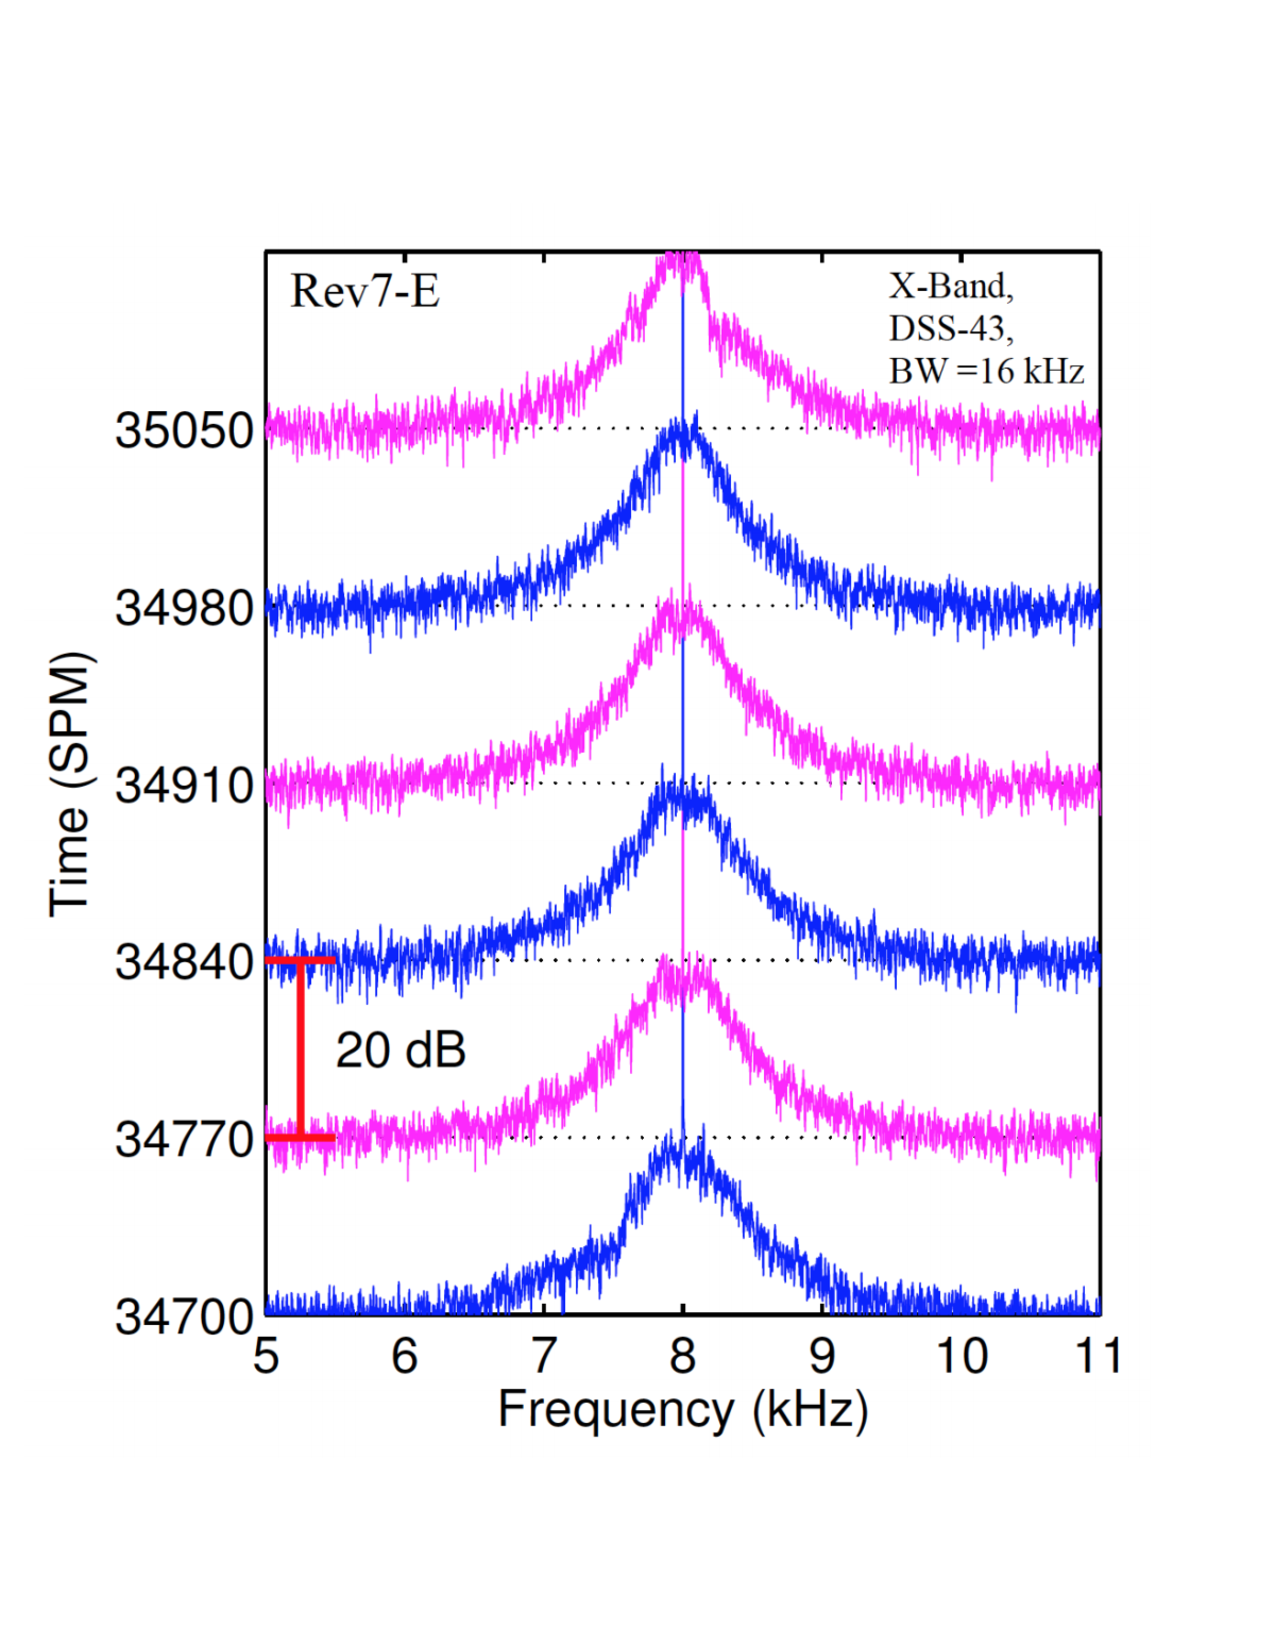
\includegraphics[%
            width=\textwidth,
            page=1,
            trim={0.0in 1.45in 0in 1.65in},
            clip
        ]{user_guide_fig_3-9.pdf}
        \caption{CRSUG Fig. 3-9}
        \label{fig:UGfig3-9_1}
    \end{subfigure}
    \begin{subfigure}[b]{0.48\textwidth}
        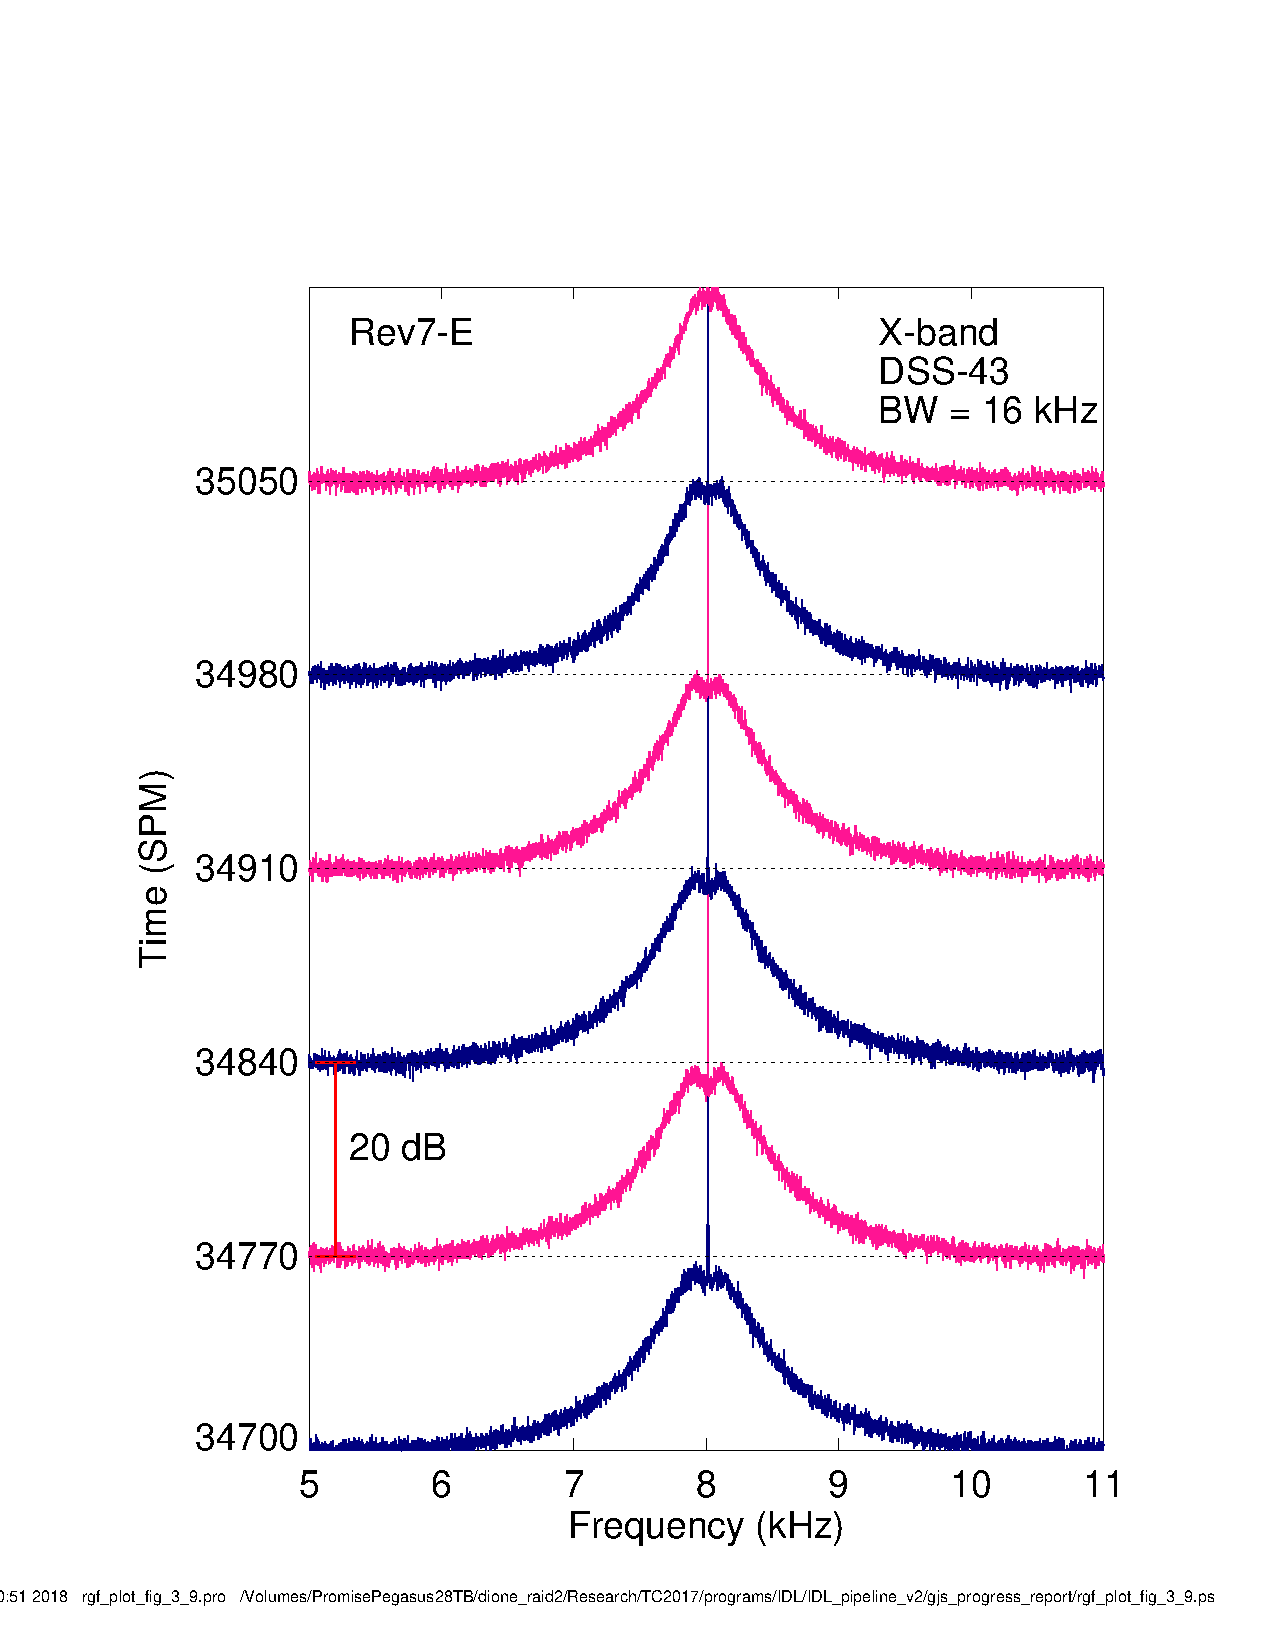
\includegraphics[width=0.9\textwidth,page = 1,trim = {0.2in 0.5in 0.2in 1.75in},clip]{rgf_plot_fig_3_9.pdf}
        \caption{Our calculation}
        \label{fig:myUGfig3-9_2}
    \end{subfigure}
\caption[Frequency estimation]{Example time sequence of Ring A spectra used to estimate the frequency offset of the direct signal from the center of the recording bandwidth.}
\label{fig:frequency}
\end{figure}
\vspace{-4ex}
\subsubsection{Frequency-Corrected Phase}
\label{subsubsec:frequency correction}
The next step in the processing is to estimate the direct signal \gls{frequency offset} of the received signal from the predicted signal. In Fig.~\ref{fig:frequencyOffset} we compare the \gls{crsug} estimation of the direct signal frequency offset for Rev007E-X43 with our results. Once again, the agreement is excellent. This is a robust test of our ability to compute the predicted \gls{sky frequency} of the received signal observed during the experiment using the reconstructed Cassini trajectory, with the expected values based on the Cassini \gls{ephemeris} available just prior to the observations. This involved adapting portions of Nicole J.~Rappaport's PREDICTS program (written in Fortran) to IDL code. Fig.~\ref{fig:frequencyOffset} shows in black the difference in predicted sky frequency using the expected Cassini trajectory and the reconstructed Cassini trajectory, which we treat as an initial estimate to the frequency offset. \par
We next refine our estimate of the frequency offset by fitting a curve to the residual between the predicted and observed frequency. In Fig.~\ref{fig:residfrequencyOffset}, we compare the example provided in the \gls{crsug} of the estimation of the residual signal frequency offset for Rev007E-X43 with our calculations. The agreement is quite good: the overall shape of the fitted function $\hat{f}_{resid}(t)$ is very similar in both figures, and the overall frequency agrees to within 0.02 Hz overall. Even the localized variations in the observed $f_{resid}(t)$ are in excellent agreement between the two independent analyses.

\begin{figure}[H]
    \centering
    \begin{subfigure}[b]{0.43\textwidth}
        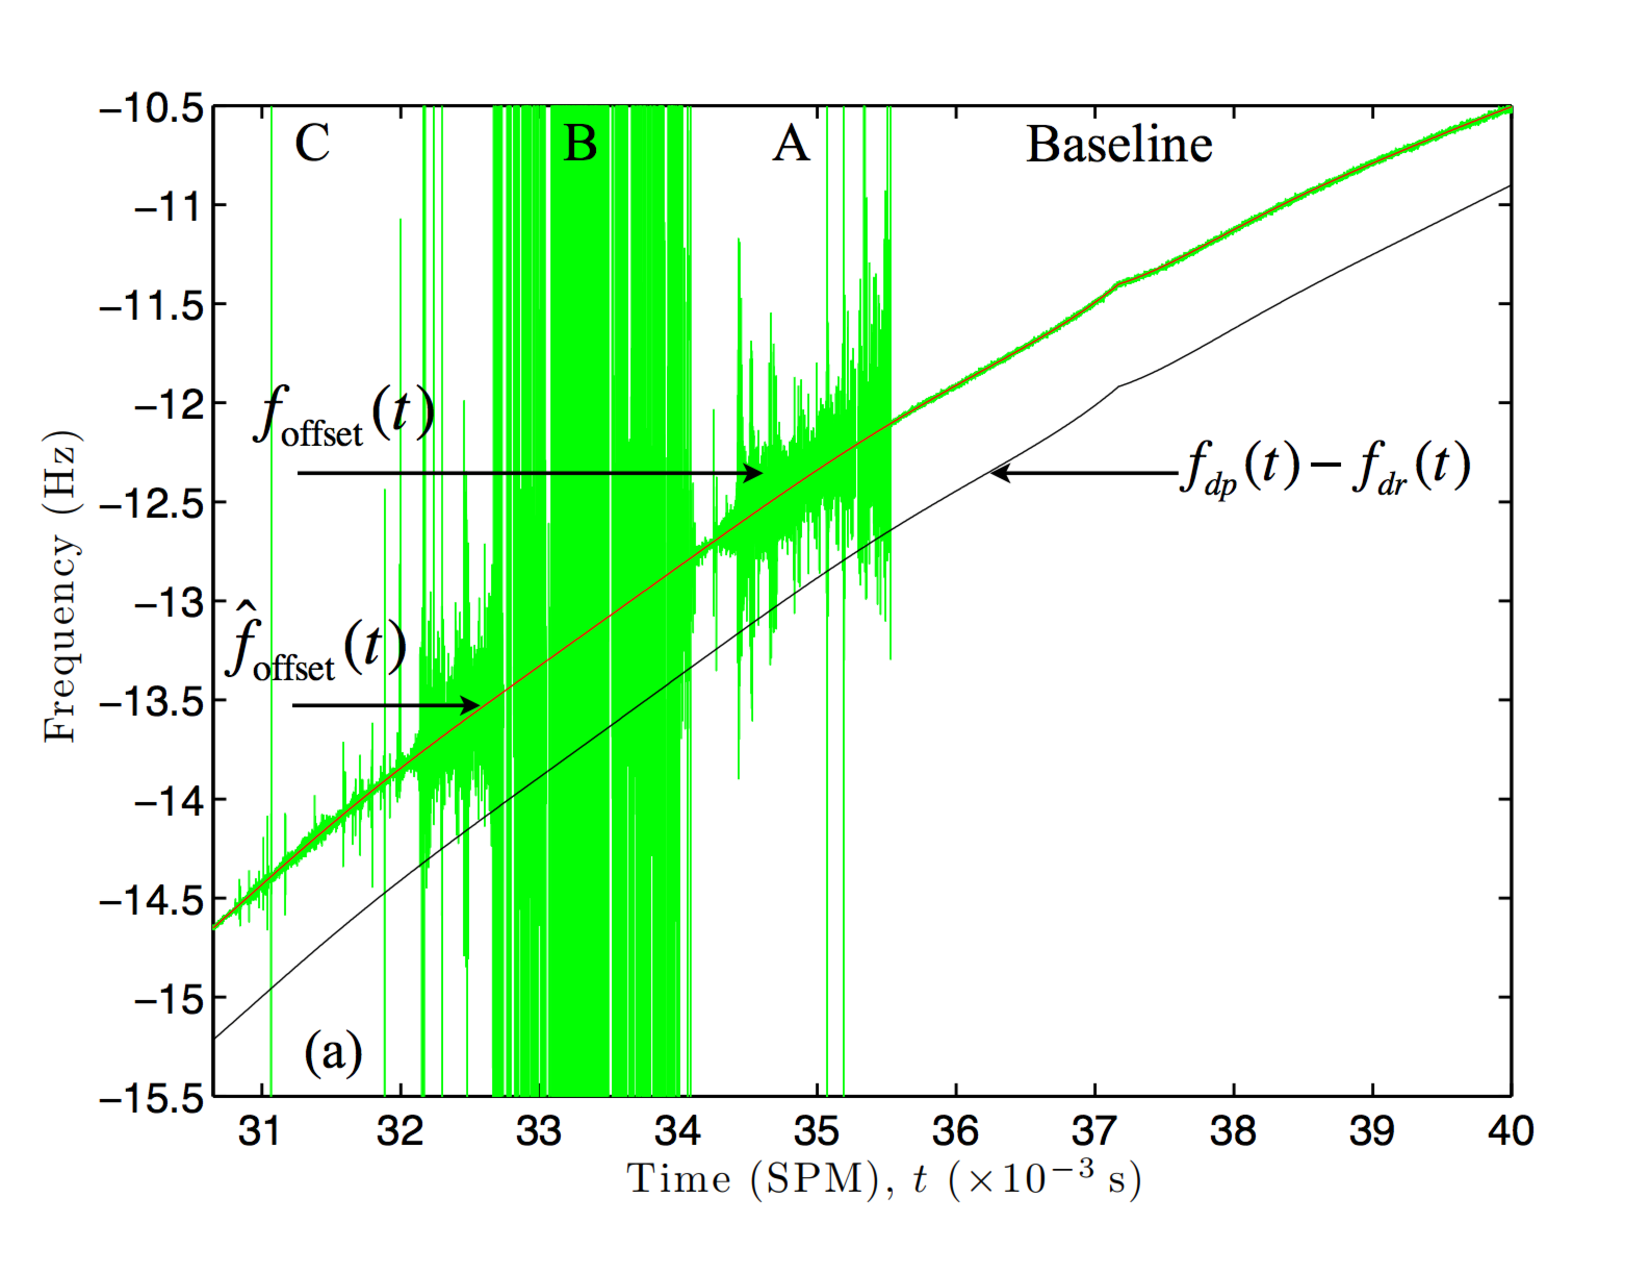
\includegraphics[width=\textwidth,page = 1,trim = {0.55in 0.5in 0.0in 0.5in},clip]{user_guide_fig_3-10_a_rotated.pdf}
        \caption{CRSUG Fig. 3-10a}
        \label{fig:UGfig3-10top}
    \end{subfigure}
    \begin{subfigure}[b]{0.47\textwidth}
        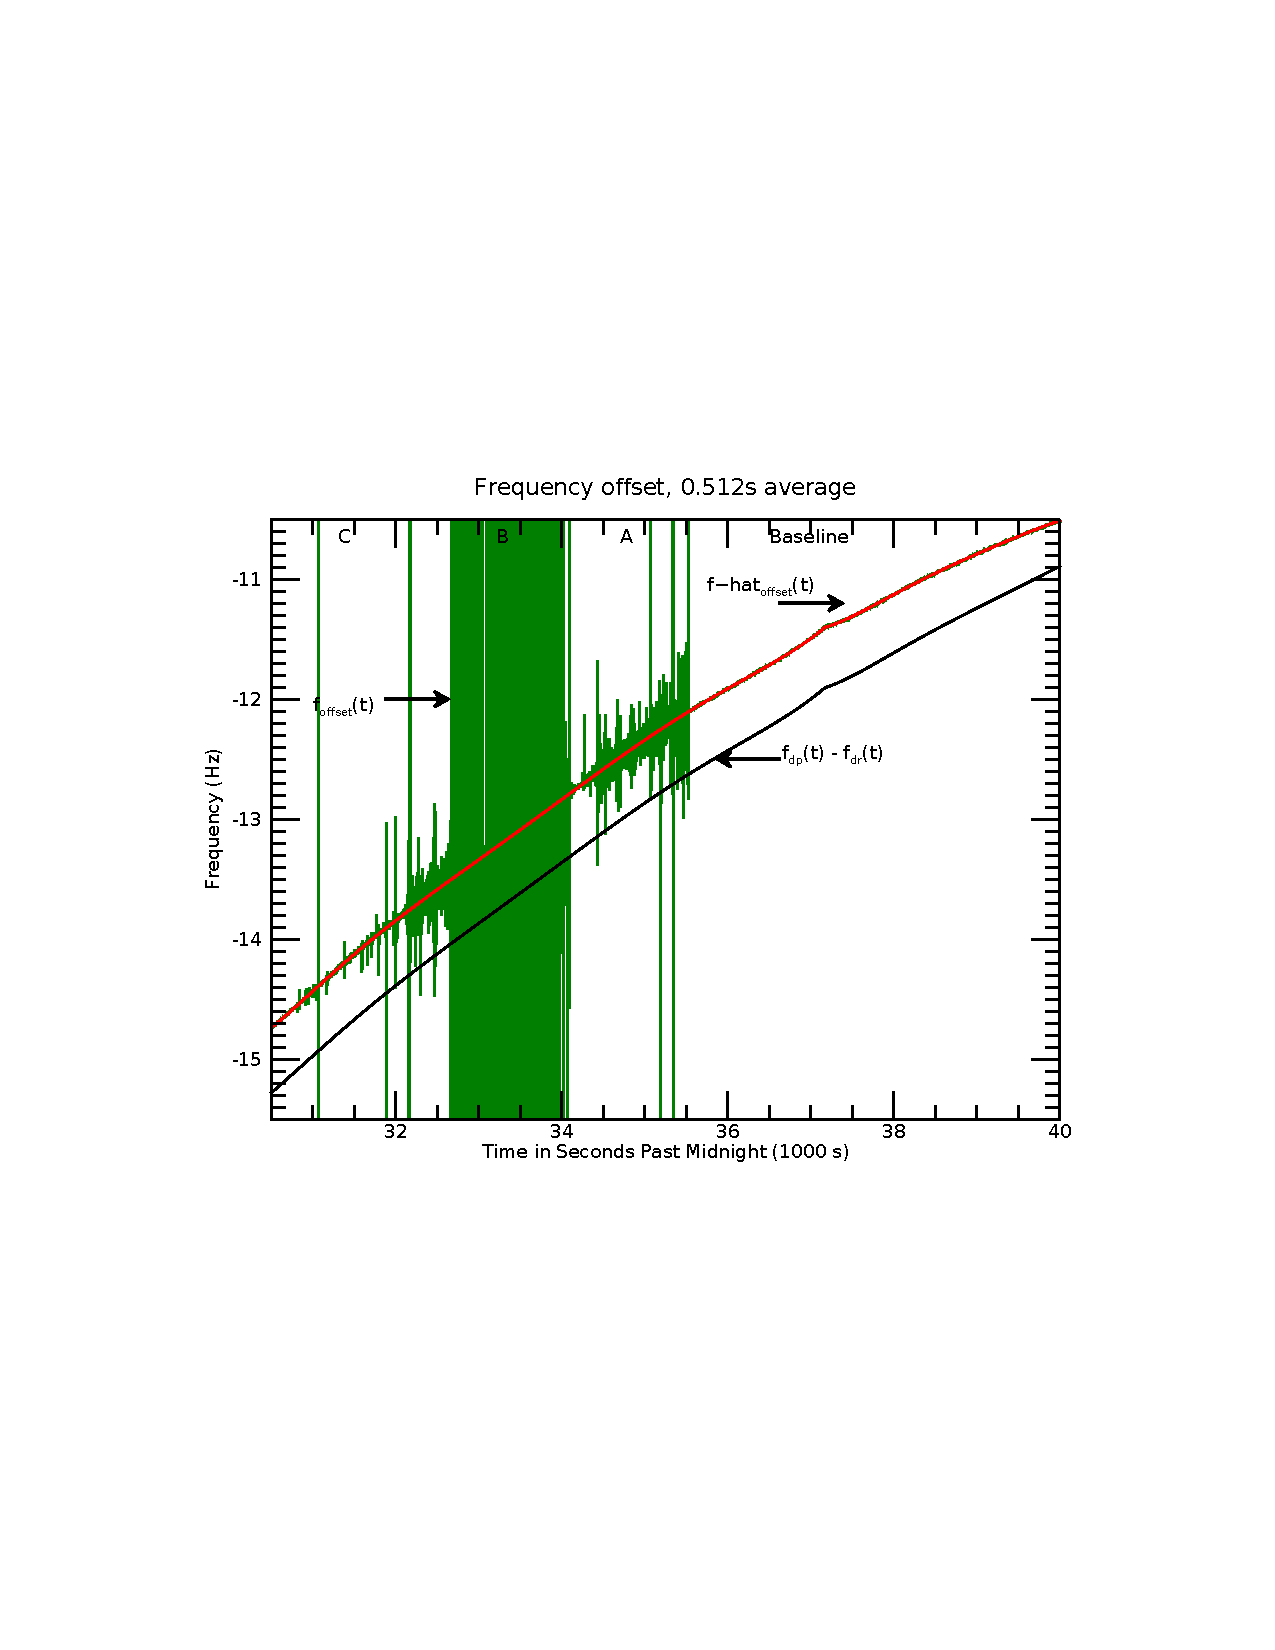
\includegraphics[width=\textwidth,trim = {1in 3.2in 0.75in 3.4in},clip]{fig_3-10_top.pdf}
        \caption{Our calculation}
        \label{fig:myUGfig3-10top}
    \end{subfigure}
    \caption[Frequency offset]{Example estimation of direct signal frequency offset. SPM is seconds past midnight 2005-05-03.}
    \label{fig:frequencyOffset}
\end{figure}
\begin{figure}[H]
    \centering
    \begin{subfigure}[b]{0.465\textwidth}
        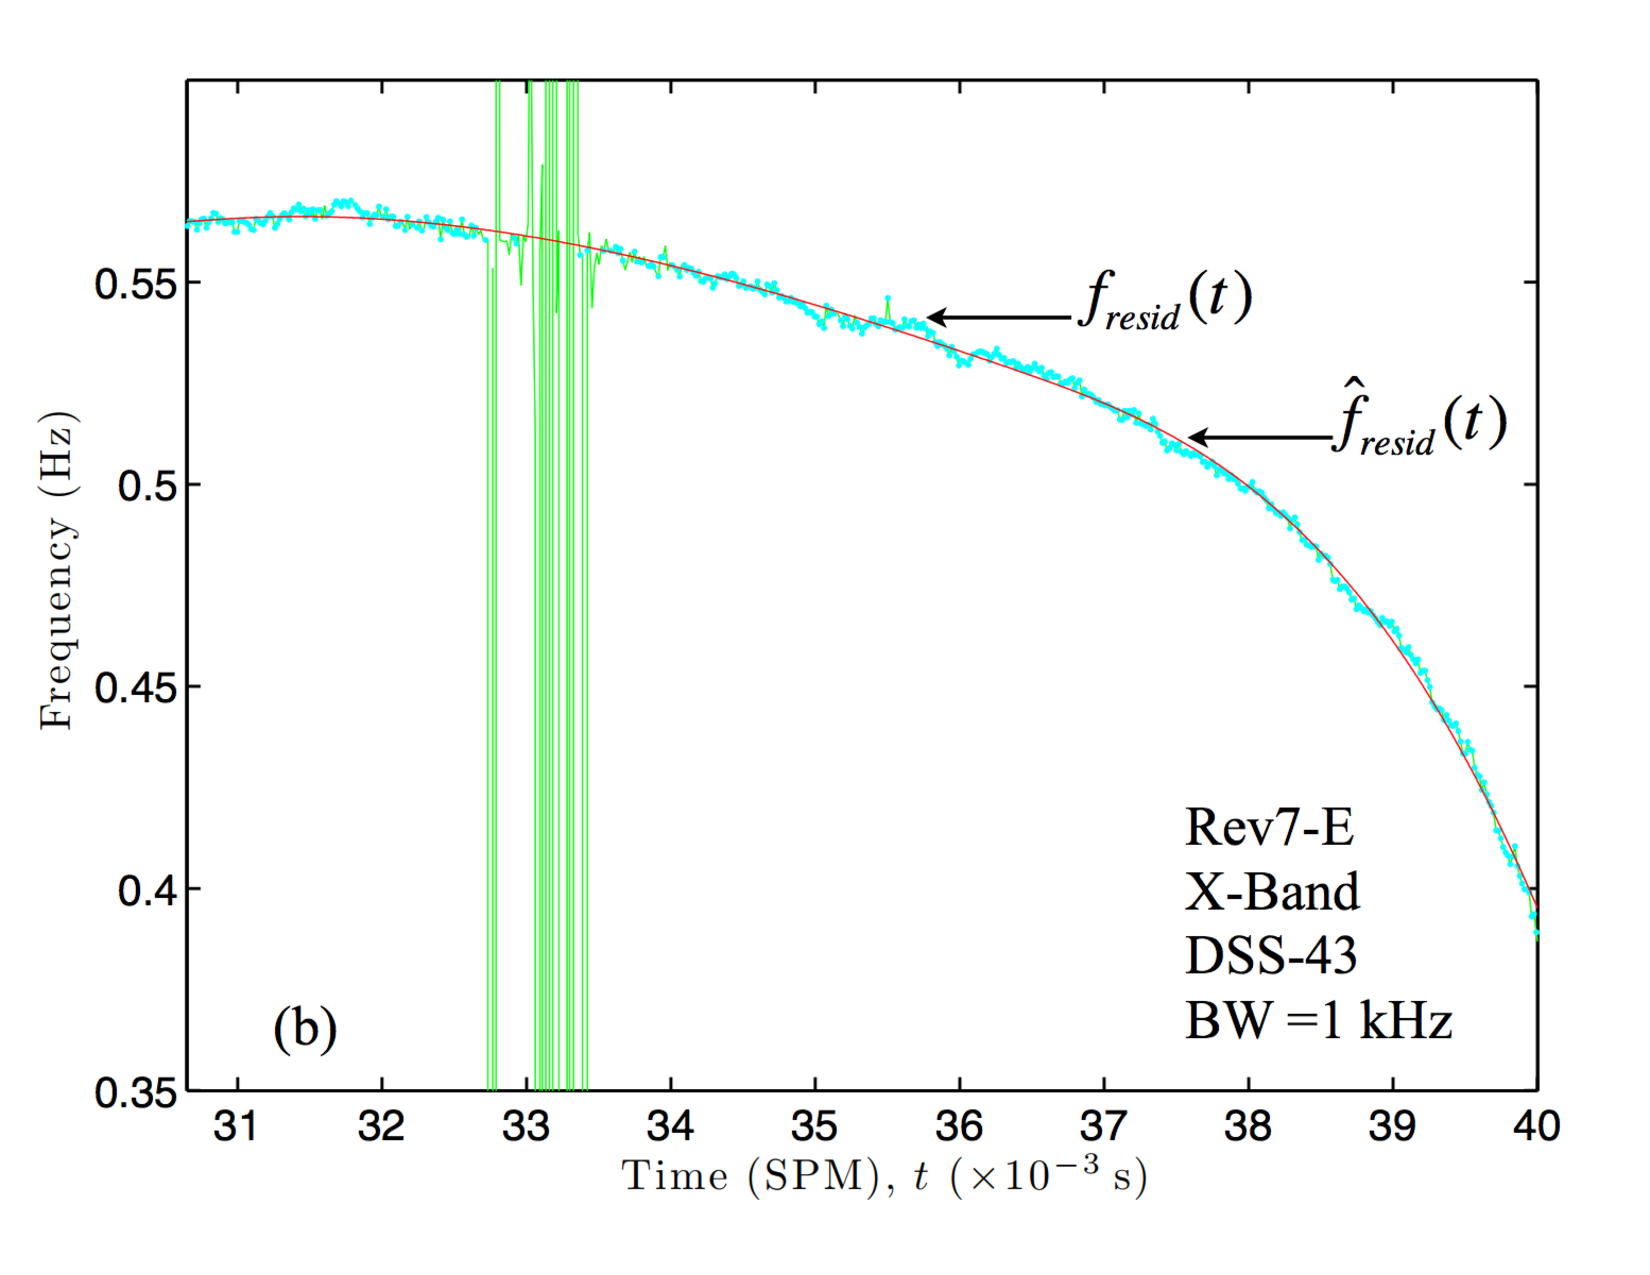
\includegraphics[width=1\textwidth,page = 1,trim = {0.05in 0.5in 0.0in 0.25in},clip]{user_guide_fig_3-10_b_rotated.pdf}
        \caption{CRSUG Fig. 3-10b}
        \label{fig:UGfig3-10bottom}
    \end{subfigure}
    \begin{subfigure}[b]{0.49\textwidth}
        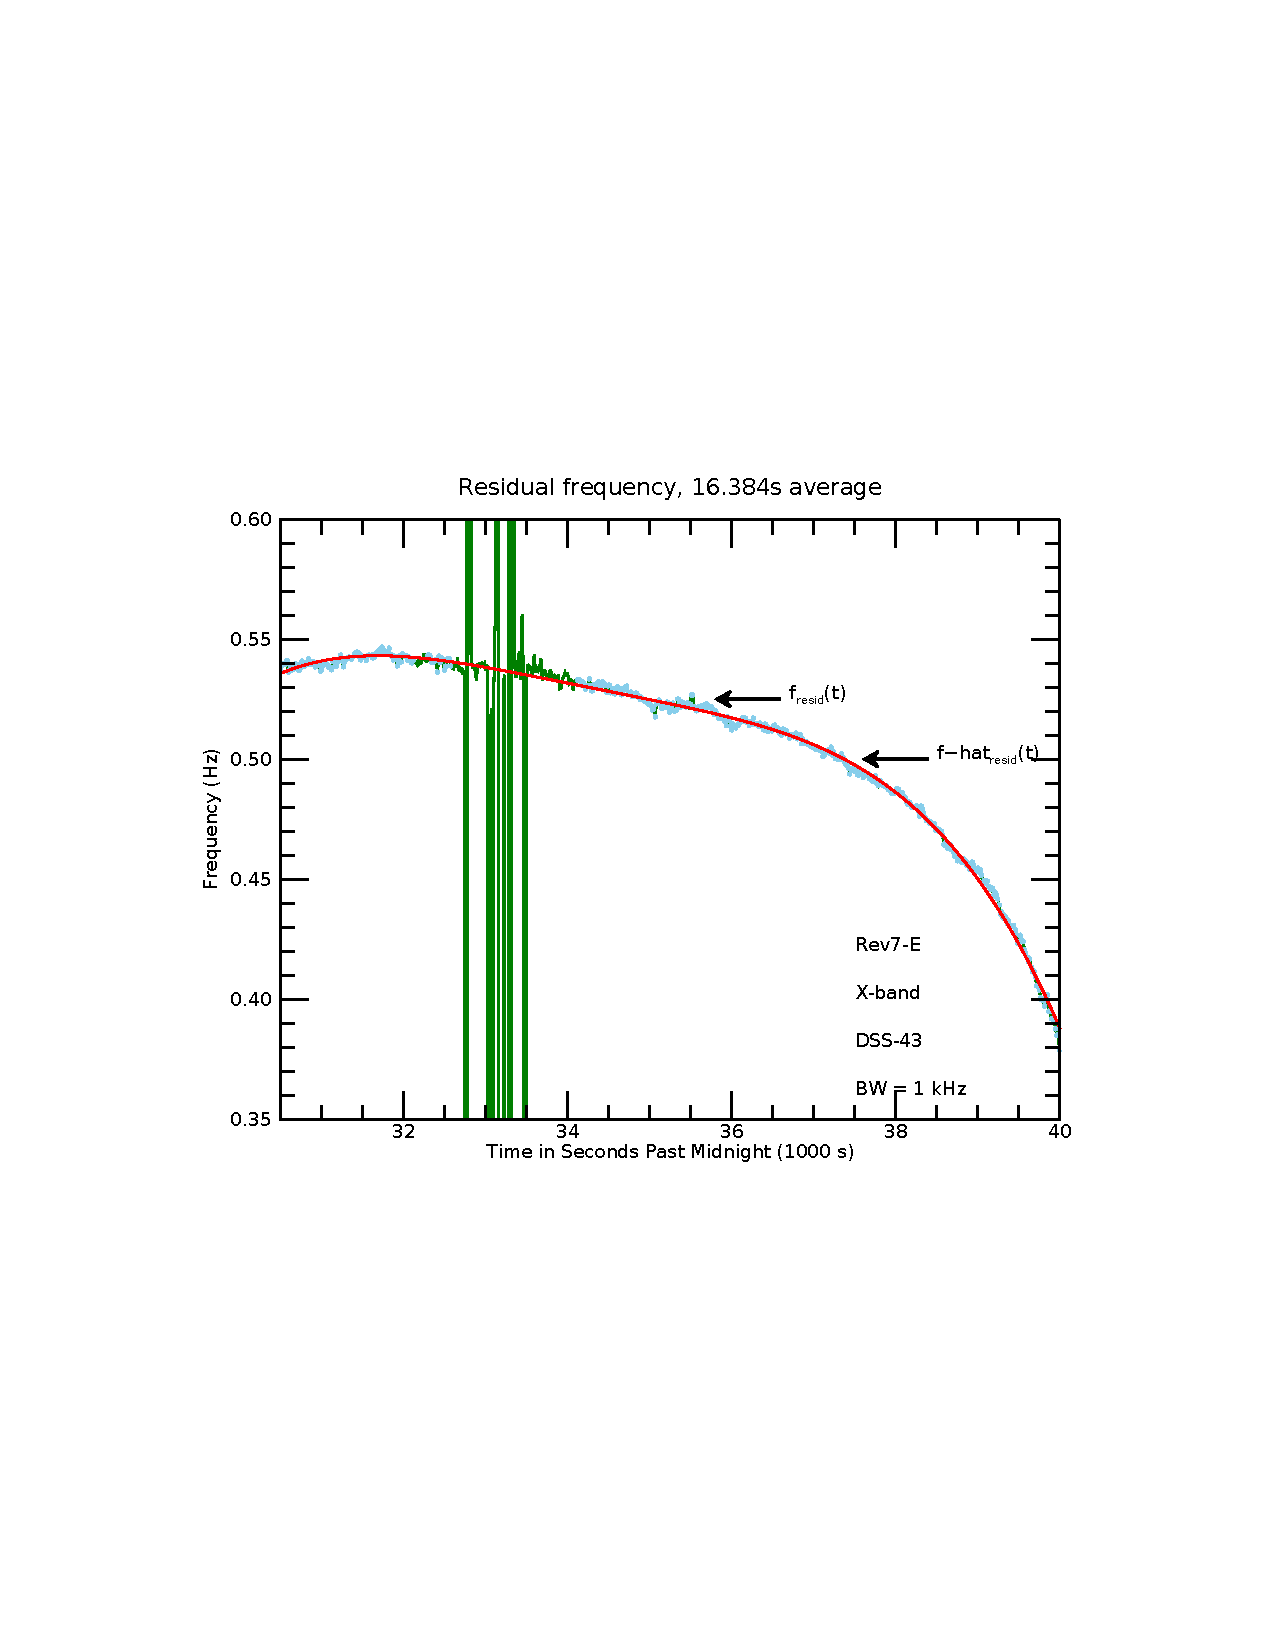
\includegraphics[width=\textwidth,trim = {1.in 3.2in 0.75in 3.1in},clip]{fig_3-10_bottom.pdf}
        \caption{Our calculation}
        \label{fig:myUGfig3-10bottom}
    \end{subfigure}
    \caption[Frequency offset]{Example estimation of residual signal frequency offset. SPM is seconds past midnight 2005-05-03.}
    \label{fig:residfrequencyOffset}
\end{figure}
\vspace{-8ex}
\subsubsection{Normalized Power}
The next step in the processing is to normalize the observed power to a free-space baseline power of unity. In Fig.~\ref{fig:power}, we compare the estimation of the normalized power $P_0(t)$ for Rev007E-X43 as shown in the \gls{crsug} with our calculation. The main ring regions (C, B, and A) are clearly visible, as labeled, followed by a free-space baseline that follows the ring \gls{occultation}. We perform a low-order \gls{least squares} \gls{spline fit} to the free-space regions, including those within the rings.\par
Specific details of the spline fit are not provided in the \gls{crsug}, but the overall shape of the normalization agrees reasonably well for the two versions. The vertical scales of the two calculations differ by a factor of about 20. Our estimate of power $P$ is the quadrature sum $P=I^2 + Q^2$ of the real and imaginary components $(I,Q)$ of the complex amplitude of the direct signal; the \gls{crsug} definition of power in terms of $I$ and $Q$ is not documented. For this comparison, we have used a Matlab implementation of the \gls{spline fit}. In our production code, we will make use of a Python library routine that performs this operation. We describe the current state of power normalization using Python routines in section \ref{subsec:conversion of software to python 3}.
\begin{figure}[H]
    \centering
    \begin{subfigure}[b]{0.46\textwidth}
        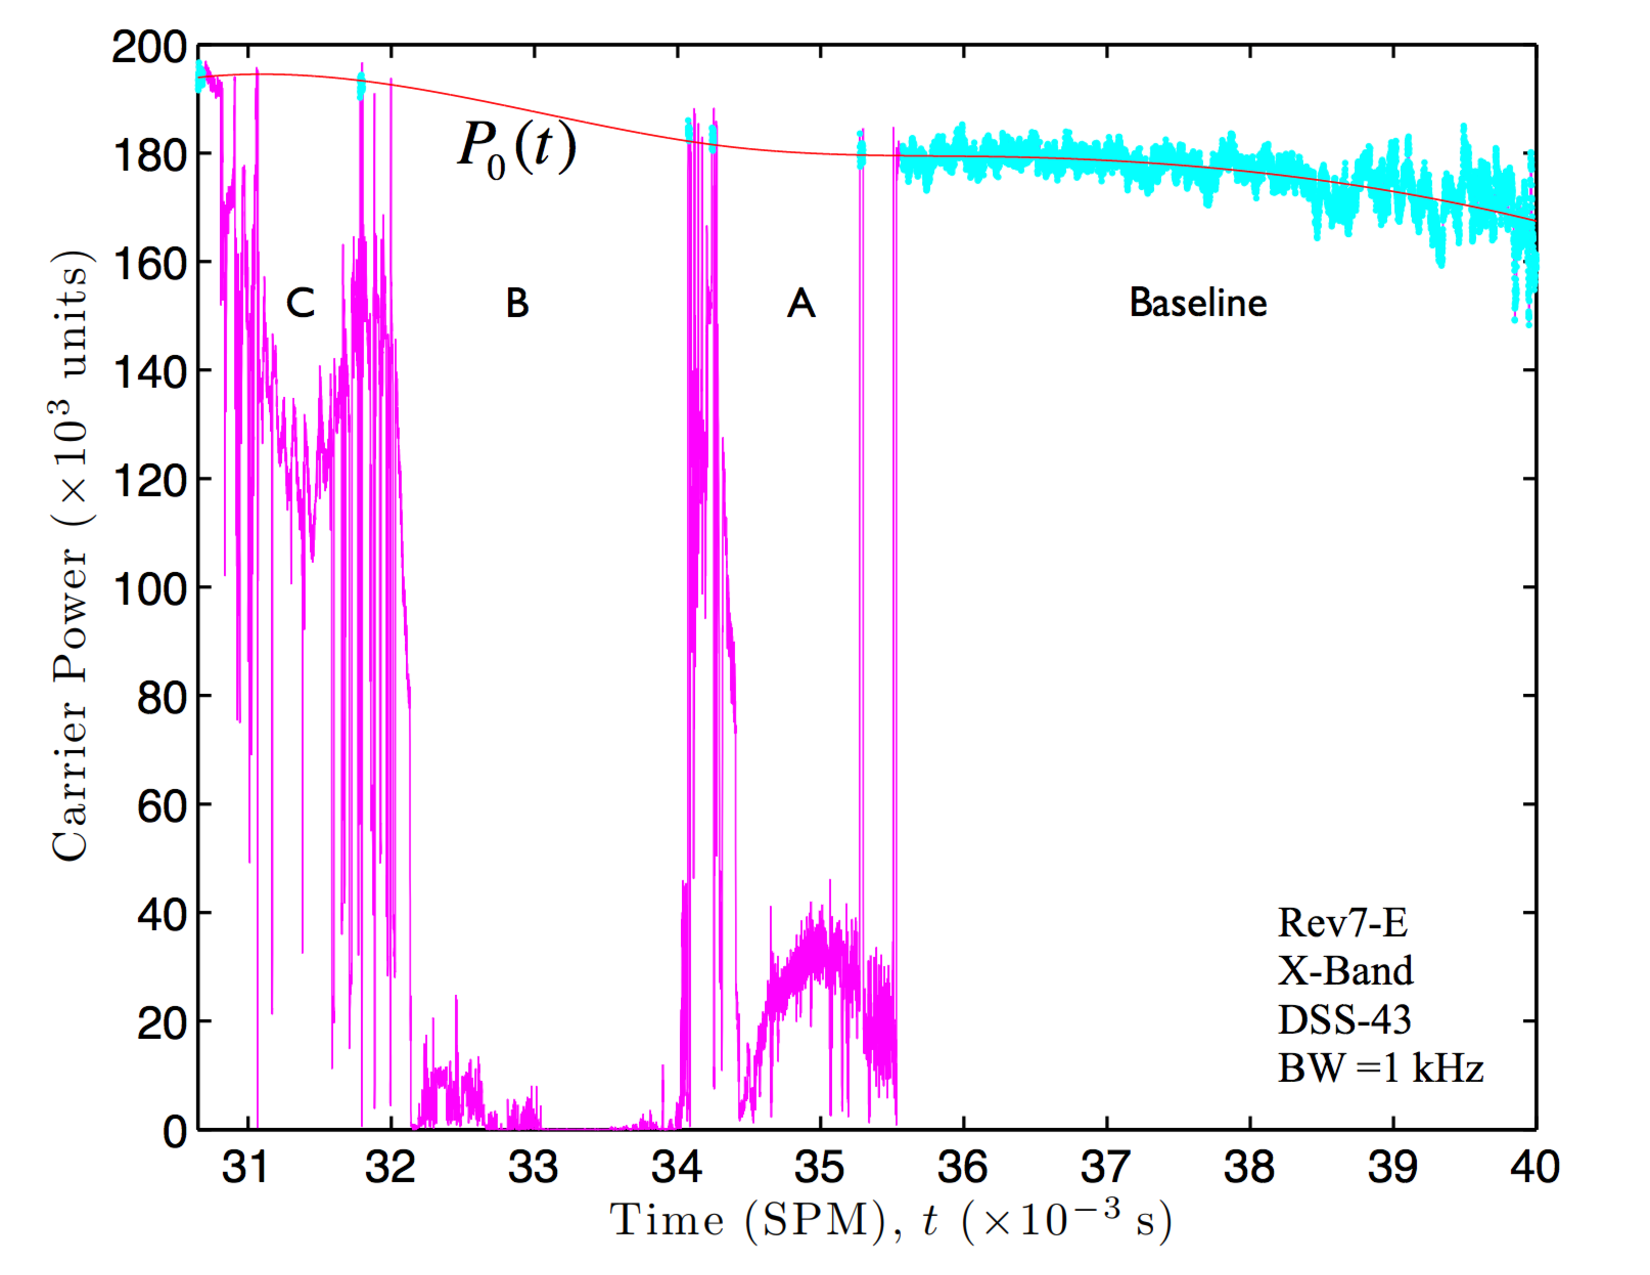
\includegraphics[width=\textwidth,page = 1,trim = {0.05in 0.25in 0in 0.2in},clip]{user_guide_fig_3-11rotated2.pdf}
        \caption{CSRUG Fig. 3-11}
        \label{fig:UGfig3-11}
    \end{subfigure}
    \begin{subfigure}[b]{0.49\textwidth}
        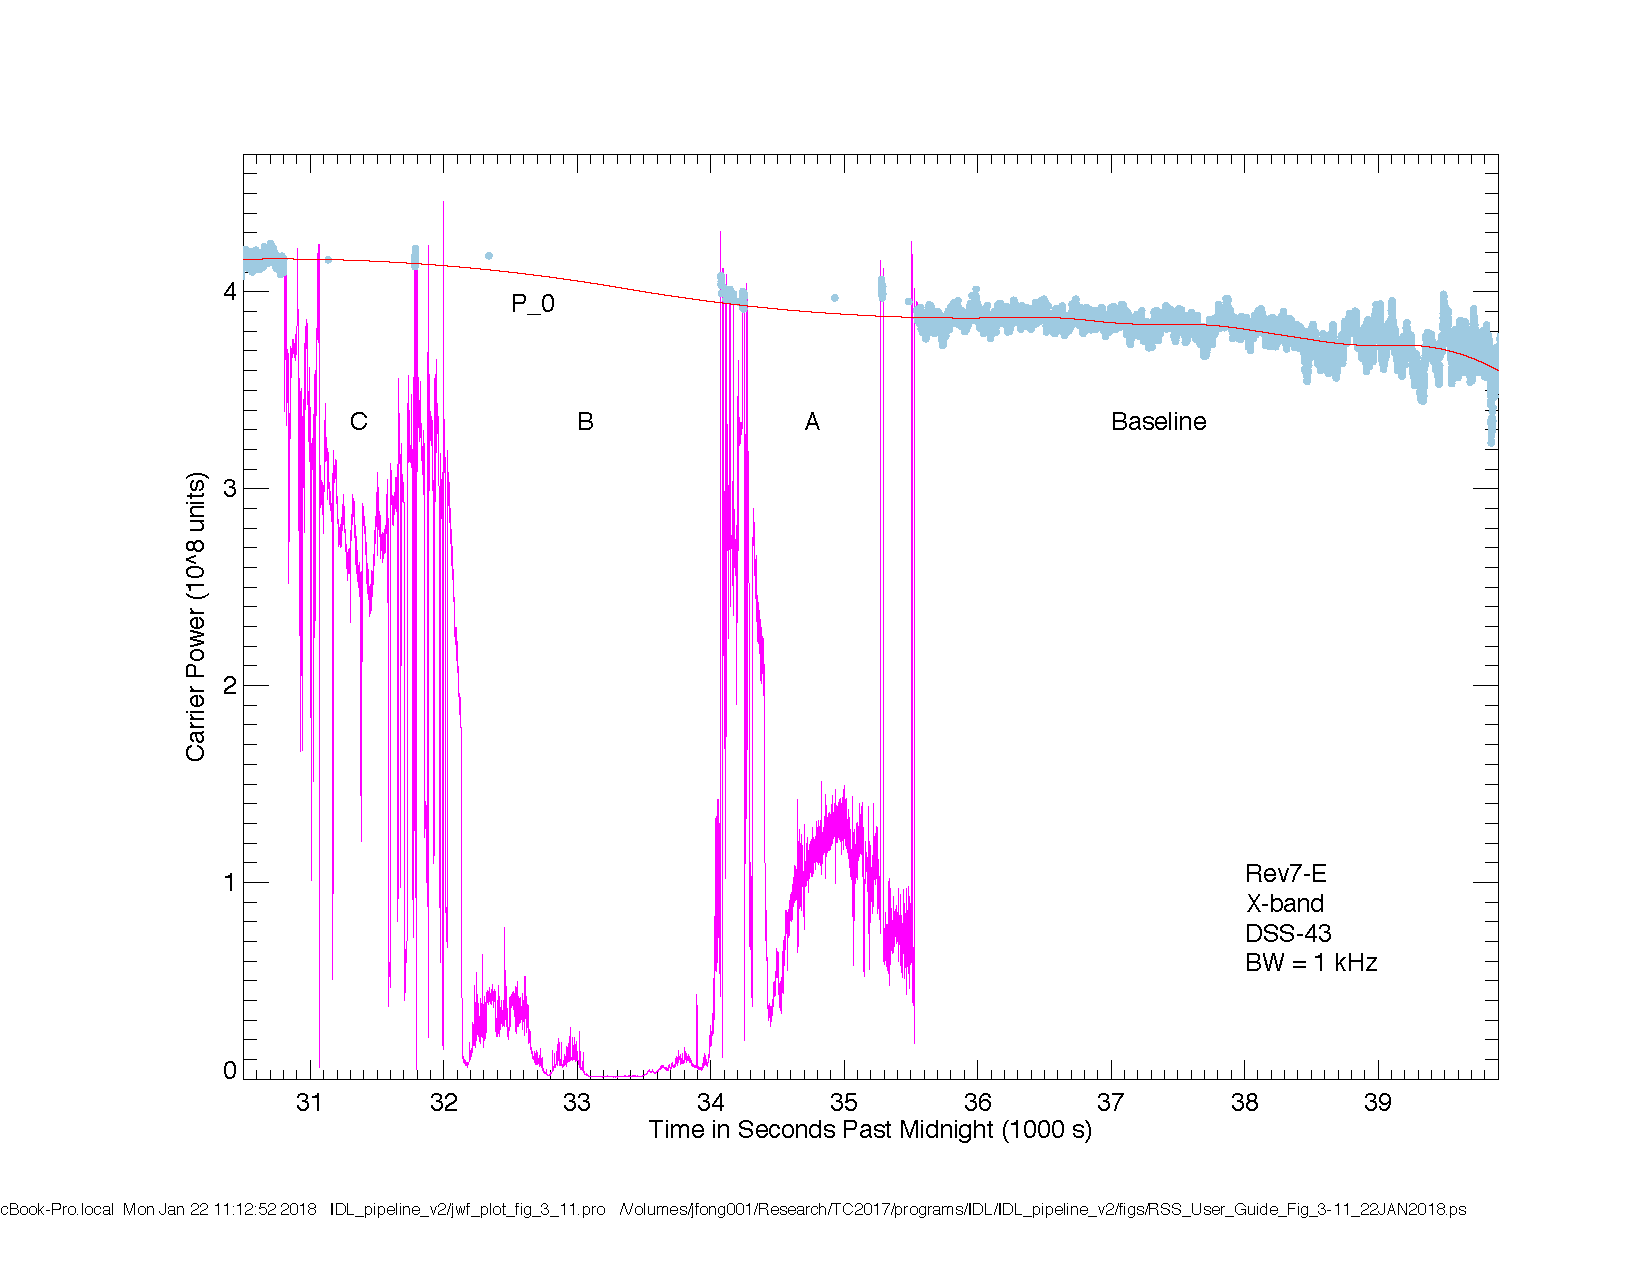
\includegraphics[width=\textwidth,page = 1,trim = {1in 0.65in 0in 0in},clip]{RSS_User_Guide_Fig_3-11_22JAN2018.pdf}
        \caption{Our calculation}
        \label{fig:fig3-11}
    \end{subfigure}
    \caption[Free space power]{Example estimation of the free-space signal power $P_0(t)$. SPM is seconds past midnight 2005-05-03.}
    \label{fig:power}
\end{figure}
\subsubsection{Calibrated Diffraction Profile}
The \gls{crsug} provides two examples of calibrated diffraction profiles and their corresponding \glspl{diffraction reconstruction}. Figure \subref{fig:UGfig3-12} shows the User Guide's \gls{optical depth} and phase profile reconstructions from \gls{x-band} diffraction-limited Rev007E Huygens Ringlet \gls{occultation} observations of 2005-05-03. The blue curves represent the measured \gls{optical depth} (upper panel) and frequency-corrected phase (lower panel) prior to diffraction correction. The diffraction fringes are quite prominent. The reconstructed optical depth and phase profiles are shown in red. Notice the sharp edges of the reconstructed profile of the Huygens ringlet at left -- the optical depth profile shows no traces of uncorrected diffraction effects. 
\begin{figure}[H]
    \centering
    \begin{subfigure}[b]{0.5\textwidth}
        \centering
        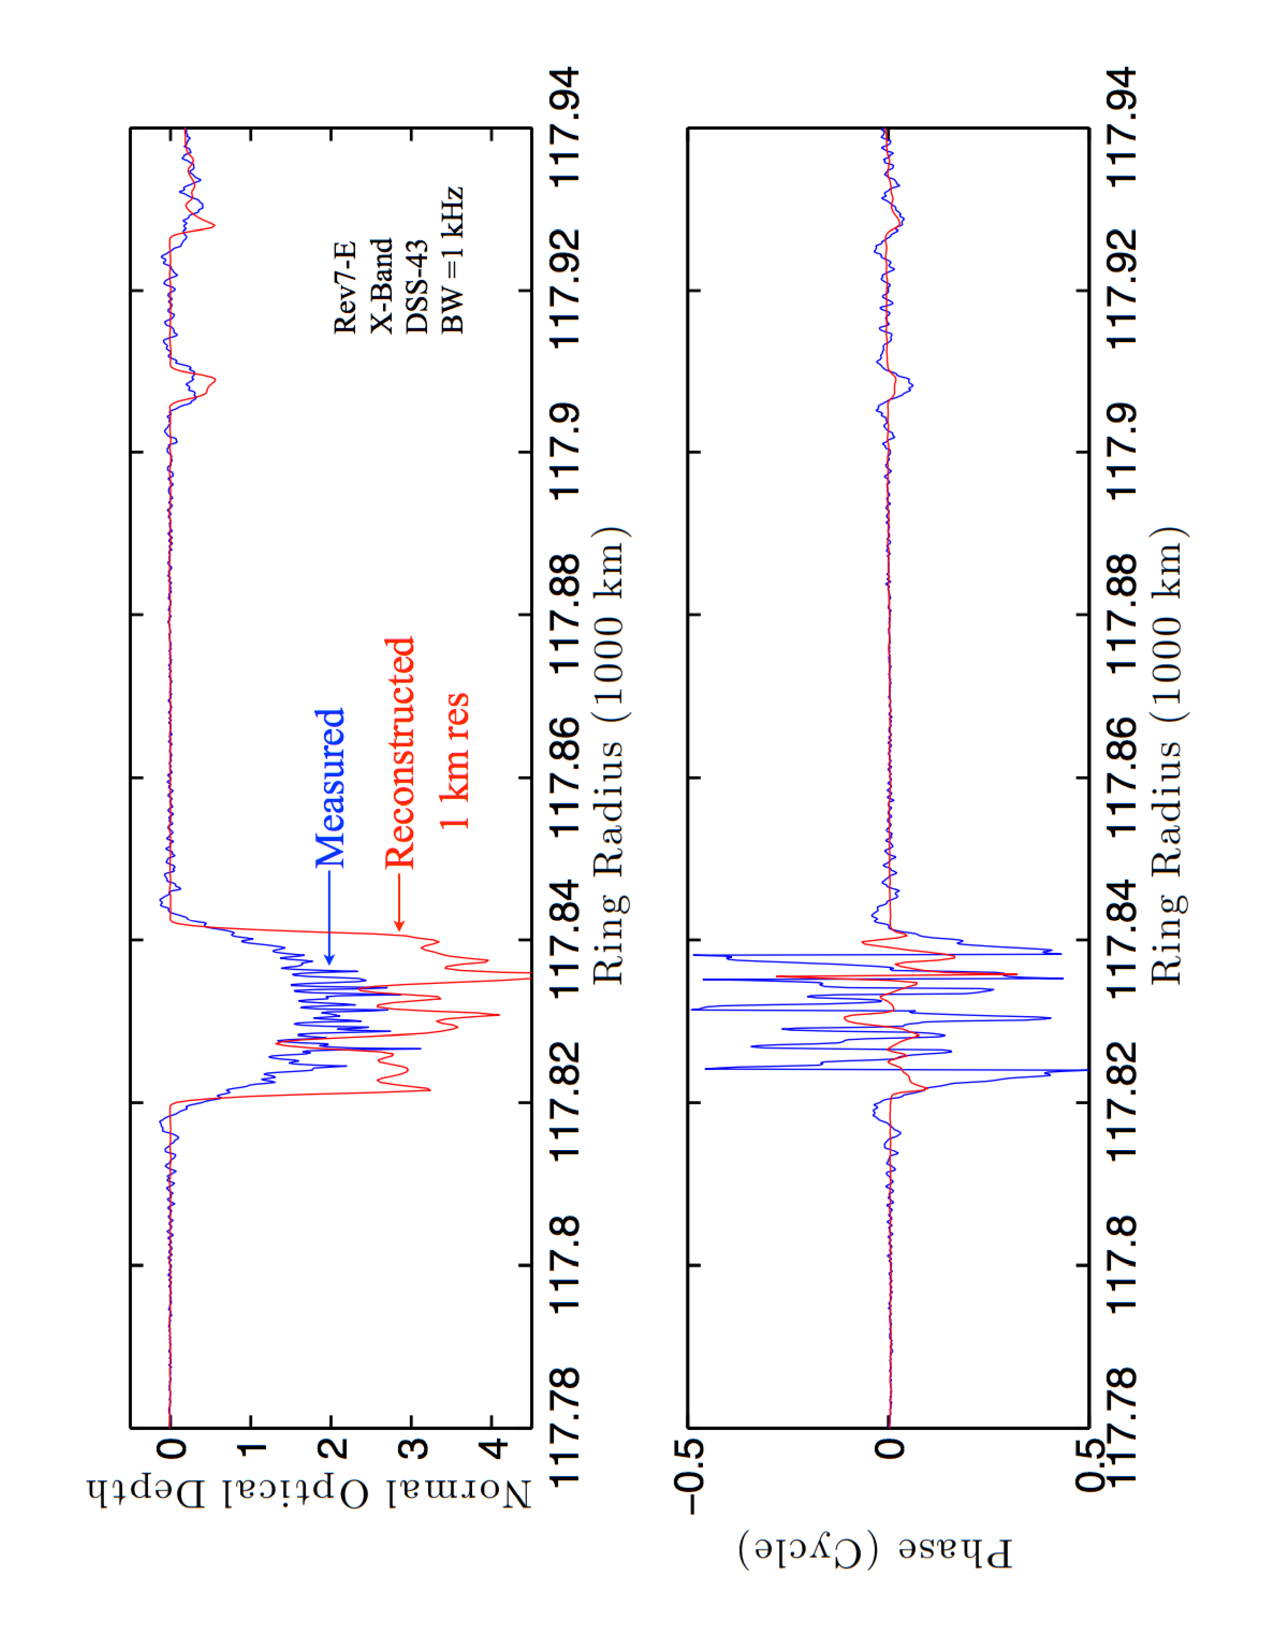
\includegraphics[angle=-90,width=\textwidth,page = 1,trim = {0.6in 0.4in 0.6in 0.8in},clip]{user_guide_fig_3-12.pdf}
        \caption{CRSUG Fig. 3-12}
        \label{fig:UGfig3-12}
    \end{subfigure}
    \begin{subfigure}[b]{0.48\textwidth}
        \centering
        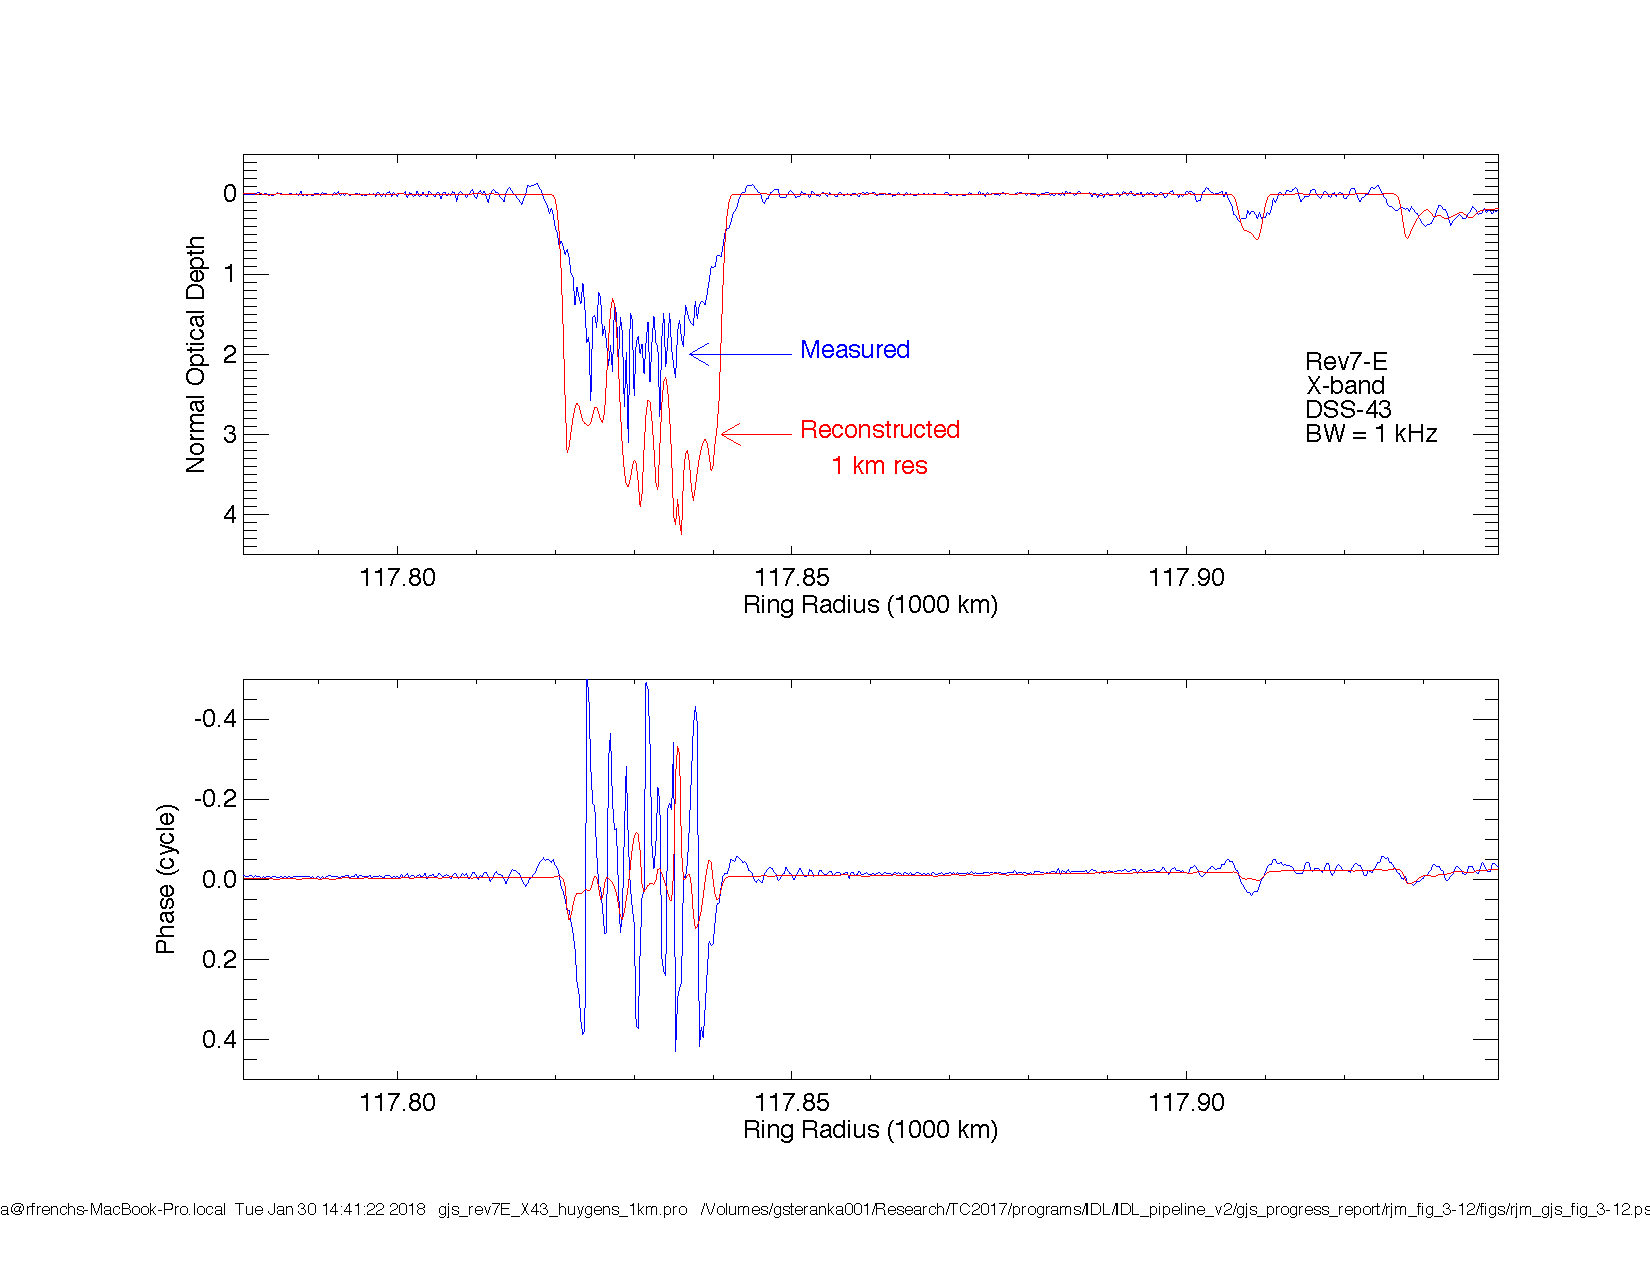
\includegraphics[width=\textwidth,page = 1,trim = {1in 0.72in 1in 0.55in},clip]{rjm_gjs_fig_3-12.pdf}
        \caption{Our calculation}
        \label{fig:myfig3-12}
    \end{subfigure}
    \caption[Reconstruction of Huygens Ringlet]{Optical depth and phase profile reconstructions of the Huygens Ringlet.}
    \label{fig:HuygensRinglet}
\end{figure}
\vspace{-4ex}
For comparison, our reconstruction is shown in Fig.~\subref{fig:myfig3-12}. For this example, we use a simple interpolation filtering scheme to convert from the raw \gls{rsr} data to the normalized diffraction pattern. For our final data pipeline, we will use the more sophisticated low-pass \gls{fir} filtering and resampling procedure described in section \ref{section:data pipeline}, but as best as can be seen by eye, our measured diffraction profiles in \gls{optical depth} and phase match those from the \gls{crsug} quite well, as do the reconstructed profiles.\par
The \gls{crsug} also provides \glspl{diffraction reconstruction} for Titan ringlet profiles processed at various resolutions, as seen in Fig.~\ref{fig:UGfig3-13}. In the top panel of the figure, the green, blue, and red curves represent optical depth at 100 m, 1 km, and 10 km processing resolution, respectively. Note how the sharpness of the reconstructed optical depth profile of the ring edge increases at higher resolutions. The bottom panel displays residual phase, using the same color scheme for the three different resolutions. All resolutions give a flat residual phase outside of the ringlet, and only the residual phase of the 10 km resolution remains flat over the ringlet.
\begin{figure}[H]
    \centering
    \begin{subfigure}[b]{0.5\textwidth}
        \centering 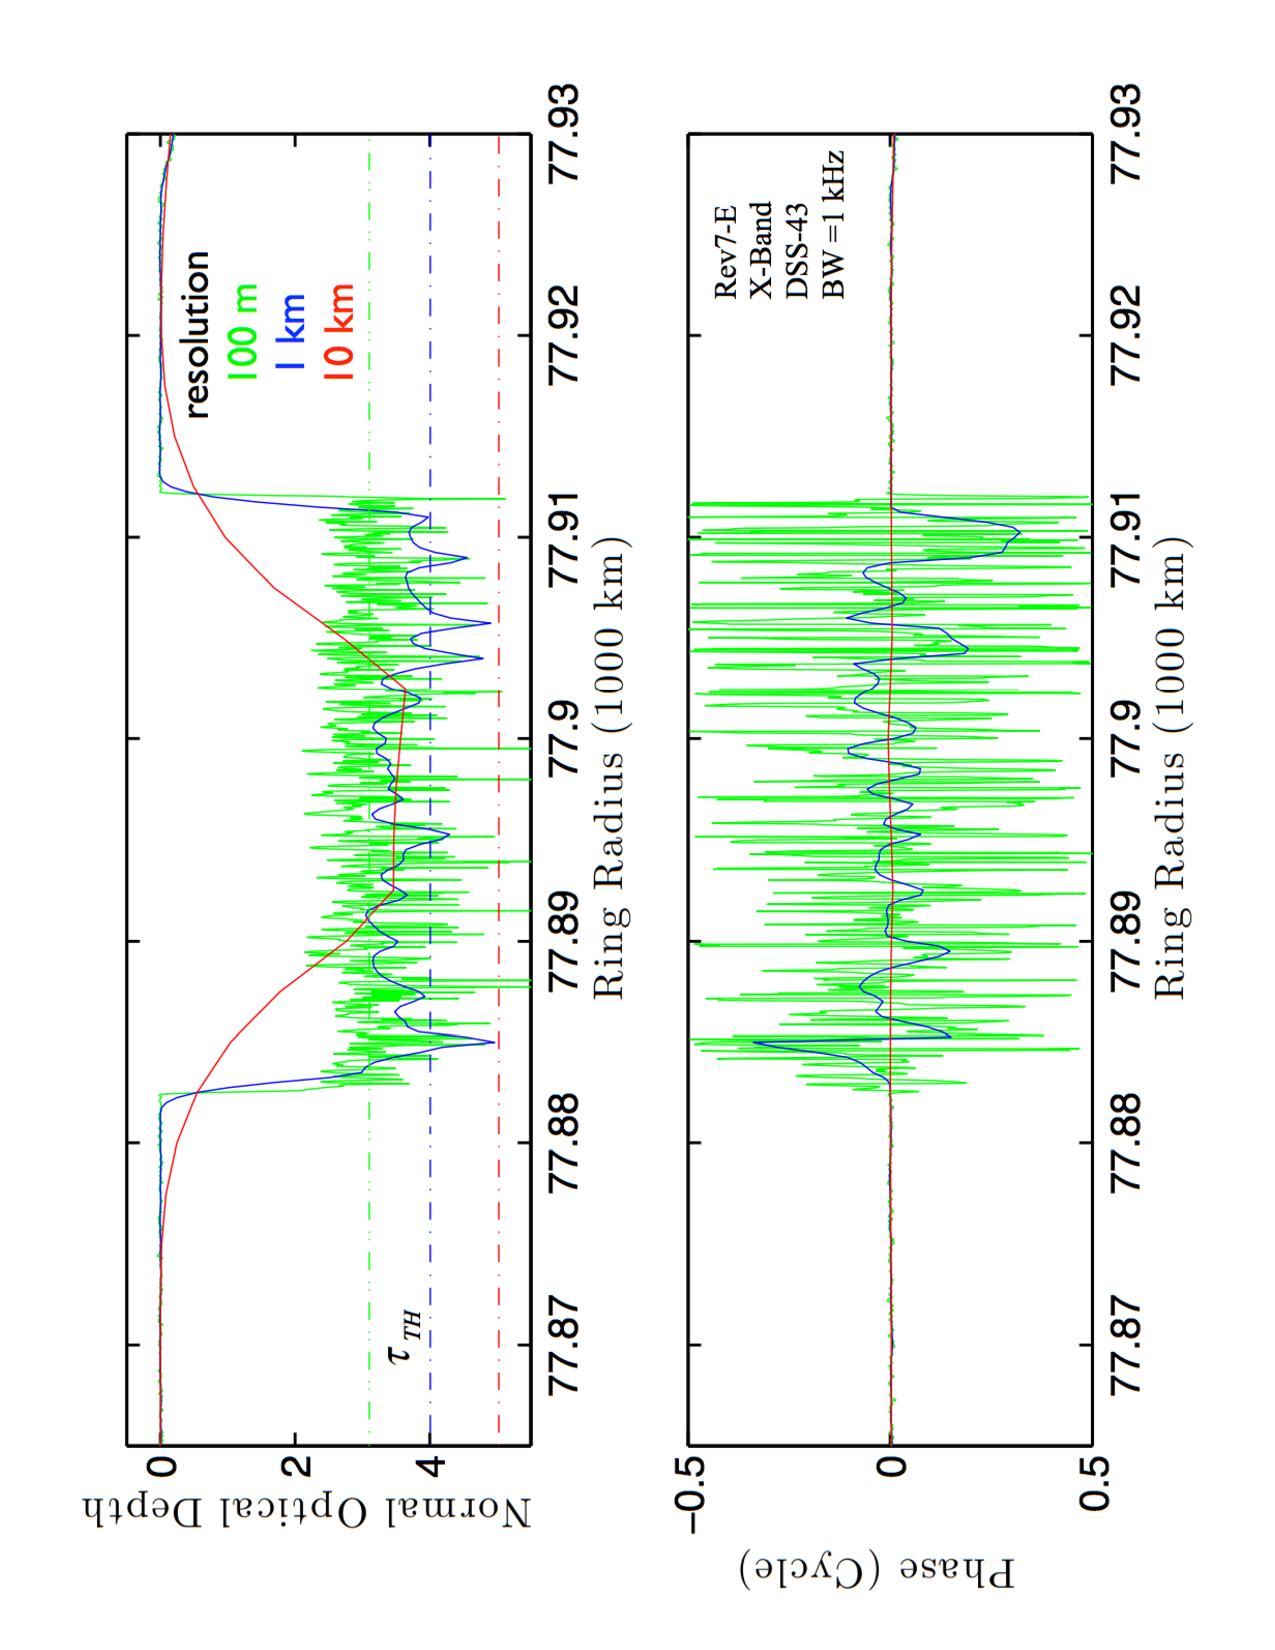
\includegraphics[angle=-90,width=0.95\textwidth,page = 1,trim = {0.8in 0.4in 0.6in 0.9in},clip]{user_guide_fig_3-13.pdf}
        \caption{CRSUG Fig. 3-13}
        \label{fig:UGfig3-13}
    \end{subfigure}
    \begin{subfigure}[b]{0.49\textwidth}
        \centering
        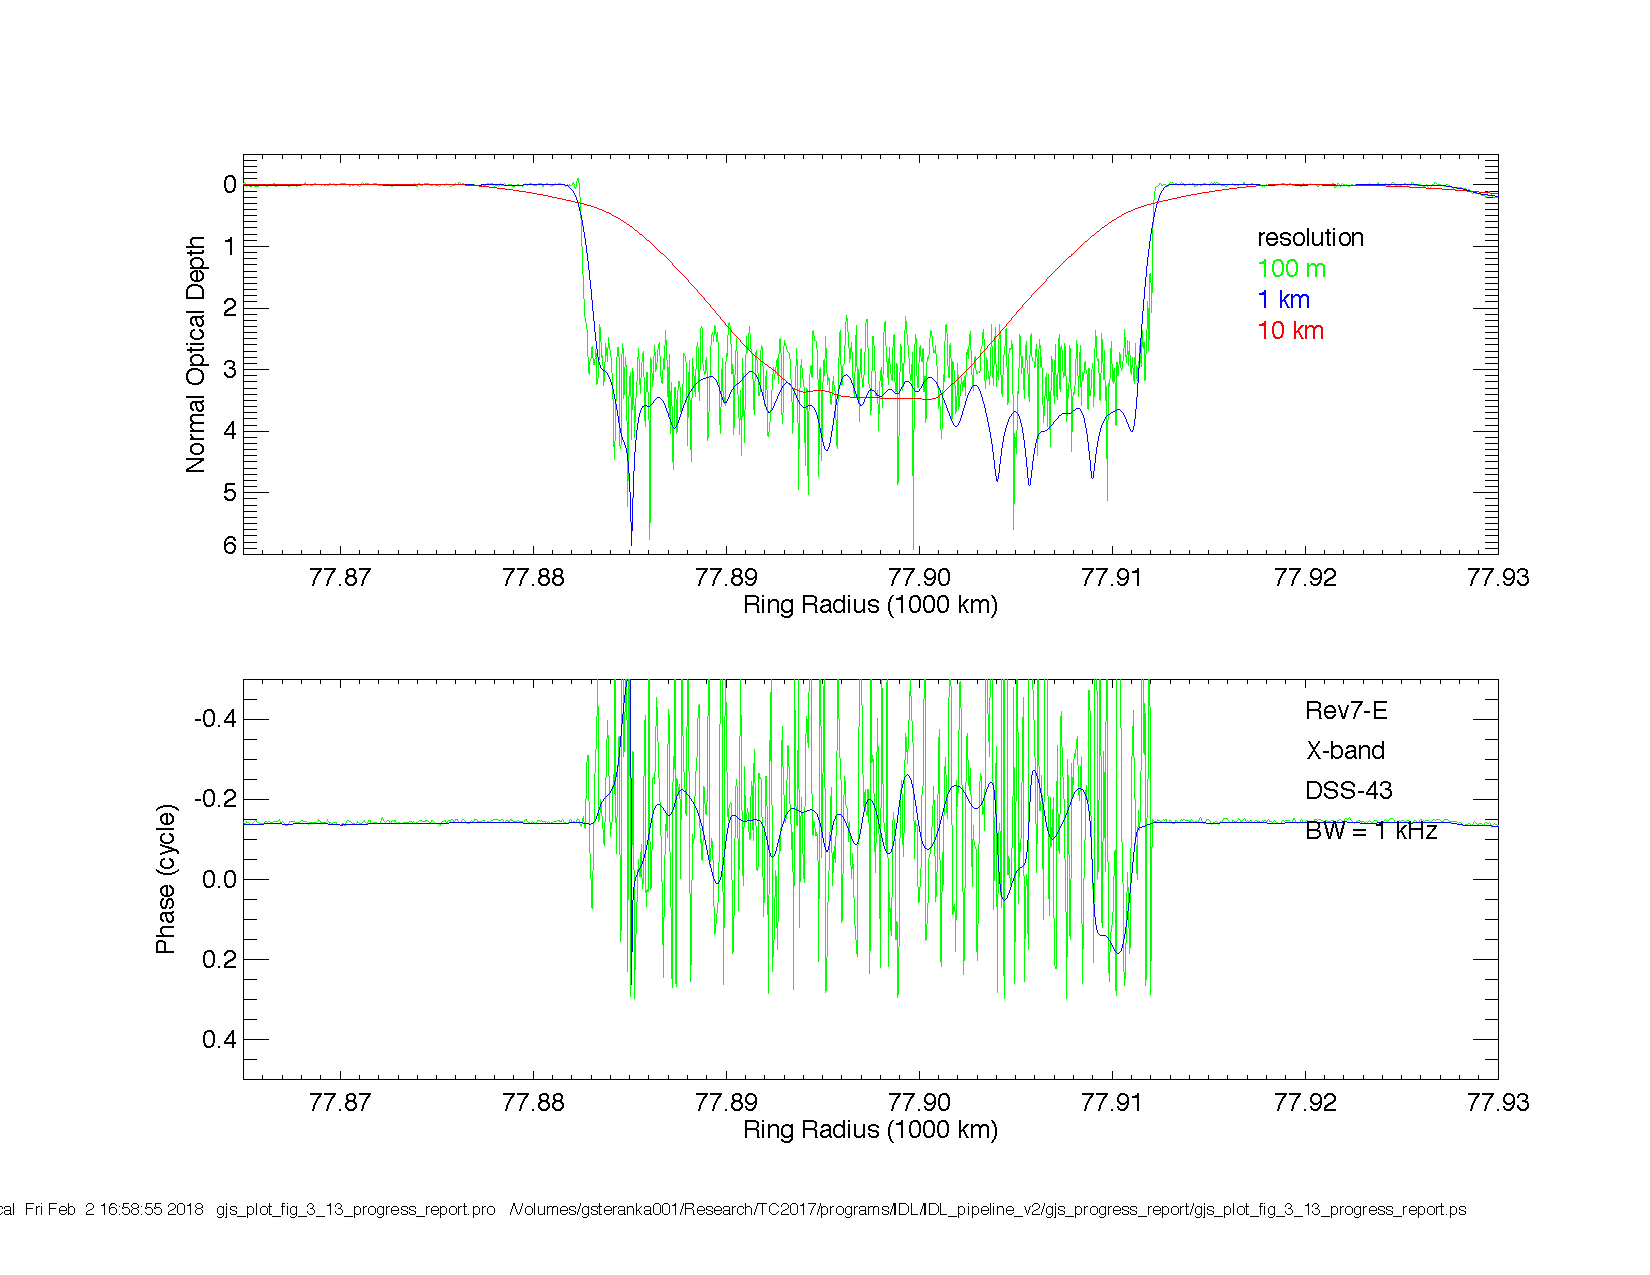
\includegraphics[width=0.95\textwidth,page = 1,trim = {1in 0.75in 1in 1in},clip]{gjs_plot_fig_3_13_progress_report.pdf}
        \caption[Titan Ringlet - our results]{Our calculation}
        \label{fig:myUGfig3-13}
    \end{subfigure}
    \caption[Titan Ringlet - CRSUG Fig.~3.13]{Optical depth and phase profile reconstructions of the Titan Ringlet.}
    \label{fig:TitanRinglet}
\end{figure}
\vspace{-4ex}
In Fig.~\subref{fig:myUGfig3-13}, we show the results of our reconstruction over the same region using the same color scheme as Fig.~\subref{fig:UGfig3-13}. The \gls{optical depth} profiles show sharper ring edges with decreasing processing resolution in much the same as those in Fig.~\subref{fig:UGfig3-13}. Additionally, the reconstructed \gls{optical depth} and residual phase profiles for 1 km resolution shows the same structure within the Titan ringlet as that found in the \gls{crsug}. We have not included lines showing our calculations of threshold optical depth, since the information in section 3.3.4.6 of the \gls{crsug} is insufficient for us to be able to reproduce the values shown. At 100~m processing resolution, our retrieved optical depth profile matches the \gls{crsug} results quite well, although both calculations show that the residual phase is noise-limited in high optical depth regions for a processing resolution of 100 m.
\subsubsection{Open Issues}
Two open issues have emerged from the comparisons with the \gls{crsug} results. First, as noted above, we are unable to reproduce the values shown for threshold optical depths. This does not affect our ability to perform accurate diffraction reconstructions, but it does affect our estimate of the uncertainties of the derived optical depths, and we will continue to explore this question.\par
A second issue concerns the normalization of the reconstructed optical depth profile, and is most evident in the \gls{diffraction reconstruction} performed at 10 km resolution. For such low-resolution profiles, the window function used in the integral equation for the complex transmittance is undersampled, resulting in an improperly normalized optical depth profile. We have corrected for this in an approximate fashion in Fig.~\subref{fig:myUGfig3-13}. As a practical matter, this issue disappears for resolutions of 1 km or better. We are actively exploring accurate normalization schemes to circumvent this problem.
\subsection{Comparison with Existing Results on the PDS}
The PDS volume \href{https://pds-rings.seti.org/viewmaster/volumes/CORSS_8xxx_lien_resolution/CORSS_8001/}{CORSS\_8001} contains geometry, calibration, and reconstructed radial profile data files for selected \gls{rss} observations. In this section, we compare the results of our pipeline to the files provided in {\tt CORSS\_8001} for Rev007 egress occultation observed at \gls{x-band} from DSS-43.
\subsubsection{Occultation Geometry}
\label{subsubsec:CSRUG_COMPARE_Occultation_Geometry}
In Fig.~\ref{fig:geometry comparison}, we compare our evaluation of \gls{occultation} geometry parameters with those shown in the \gls{pds} \href{https://pds-rings.seti.org/holdings/volumes/CORSS_8xxx_lien_resolution/CORSS_8001/EASYDATA/Rev07E_RSS_2005_123_X43_E/Rev07E_RSS_2005_123_X43_E_Summary.pdf}{EASYDATA summary}, where our calculations are shown in solid blue and the values from {\tt RSS\_2005\_123\_X43\_E\_GEO.TAB} are plotted in dashed red. Our results are virtually identical if we use the \gls{kernel} list from the geometry label file. If instead we use the planetary constants kernel appropriate for the spacecraft trajectory \gls{ephemeris} kernel, our results show discernible differences, but none of them are large enough to produce significant systematic errors in the derived optical depth profiles, other than in absolute ring radius, which is affected by the adopted planetary pole direction. Aside from this, the only noticeable discrepancy is the \gls{ring opening} angle $B$, but that can be accounted for by using \gls{ert} (green curve) instead of ring event time (blue curve) for the calculation. Again, as a practical matter, the two results are effectively identical. In short, all of our geometric calculations match those on the \gls{pds} to a high degree of accuracy. 
\begin{figure}[t]
    \centering
    \begin{subfigure}[b]{0.49\textwidth}
        \includegraphics[width=\textwidth,page = 2,trim = {0.75in 0.5in 0.2in 0.5in},clip]{Rev007_E_comparison_geo.pdf}
        \label{fig:geo_comp_p1}
    \end{subfigure}
    \begin{subfigure}[b]{0.49\textwidth}
        \includegraphics[width=\textwidth,page = 3,trim = {0.75in 0.5in 0.2in 0.5in},clip]{Rev007_E_comparison_geo.pdf}
        \label{fig:geo_comp_p2}
    \end{subfigure}\vspace{-2ex}
    \caption[Geometry comparison]{Our version of Figure 1 in the \gls{pds} EASYDATA summary PDF, with our values plotted in solid blue and values from PDS file RSS\_2005\_123\_X43\_E GEO.TAB plotted in dashed red. The solid green line is our calculation of ring opening angle using Earth-received time instead of ring event time. Clockwise, starting in top left panel: difference between observed event time and ring event time $t_{OET}-t_{RET}$, Fresnel scale $F$, impact radius $R_{impact}$, spacecraft position $(R_{x}, R_{y}, R_{z})$, spacecraft velocity $(v_{x}, v_{y}, v_{z})$, ring intercept azimuthal velocity $\rho\dot{\phi}_{RL}$, ring intercept radial velocity $\dot{\rho}$, spacecraft to ring intercept distance $D$, ring opening angle $B$, observed ring azimuth $\phi_{ORA}$, ring longitude $\phi_{RL}$, ring radius $\rho$, and difference between ring event time and spacecraft event time $t_{RET}-t_{SET}$.}
    \label{fig:geometry comparison}
\end{figure}
\subsubsection{Calibration Files}
\label{subsubsec:calibration_files}
The Rev007E calibration file {\tt RSS\_2005\_123\_X43\_E\_CAL.TAB} includes \gls{sky frequency} $f_{sky}$, residual frequency $f_{resid}$, and free-space power ($P_{free}$) as a function of \gls{ert}. Our \gls{sky frequency} calculation matches that in the \gls{pds} to a fractional error of order $10^{-11}$, while our fit to the residual frequency matches to a fractional error of order $10^{-2}$. This difference can be reduced if we lower our \gls{uso} frequency $f_{\textrm{USO}}$ by roughly 0.02 Hz, but $f_{\textrm{USO}}$ will then be inconsistent with the values provided on the \href{https://atmos.nmsu.edu/pdsd/archive/data/co-s-rss-1-sroc1-v10/cors_0108/calib/uso_060109.txt}{PDS}. As a practical matter, these slight differences have a negligible effect on the derived \gls{optical depth} profiles after \gls{diffraction reconstruction}.\par
Our calibration curve for free-space power is a \gls{least squares} \gls{spline fit} to the observed power in free-space regions and is calculated in terms of \gls{in-phase} (I) and \gls{quadrature-phase} (Q). Our $P_{free}$ is on order of $10^{8}$ times greater than the \gls{pds} value, but as seen above in Fig.~\subref{fig:UGfig3-11}, the trend and shape of our fit matches the \gls{crsug} very well, and once we normalize our frequency-corrected observations, our agreement with the \gls{pds} diffraction-corrected profiles is excellent, as shown in Fig.~\ref{fig:Maxwell Reconstruction}.
\subsubsection{Diffraction-Corrected Ring Profiles}
Both 1 km and 10 km-resolution reconstructed \gls{optical depth} profiles are available on the \gls{pds} in the data file {\tt RSS\_2005\_123\_X43\_E\_TAU\_XXKM.TAB}, where {\tt XX} represents the resolution in kilometers, along with other geometric parameters as a function of ring radius ($\Delta\rho$, $\phi_{RL}$, $\phi_{ORA}$, $B$). We can reproduce the geometry calculations $\phi_{RL}$, $\phi_{ORA}$, and $B$ extremely well, as seen in section \ref{subsubsec:CSRUG_COMPARE_Occultation_Geometry}. We can also reproduce the radius correction $\Delta\rho$ if we use the along-track timing offset provided in optical depth label file. (The only parameter from this data file that we have been unable to reproduce is the optical depth threshold $\tau_{thresh}$, as we mentioned above.) In Fig.~\ref{fig:Maxwell Reconstruction}, we compare the 1-km resolution diffraction-corrected \gls{maxwell ringlet} profile on the \gls{pds} with our independent results from our own Fresnel inversion. Our power calculations differ from the \gls{pds} values, on average, by less than 1\%. The \gls{optical depth} profile also agrees very well, both in detailed shape and in overall signal level.
\begin{figure}[H]
    \centering
    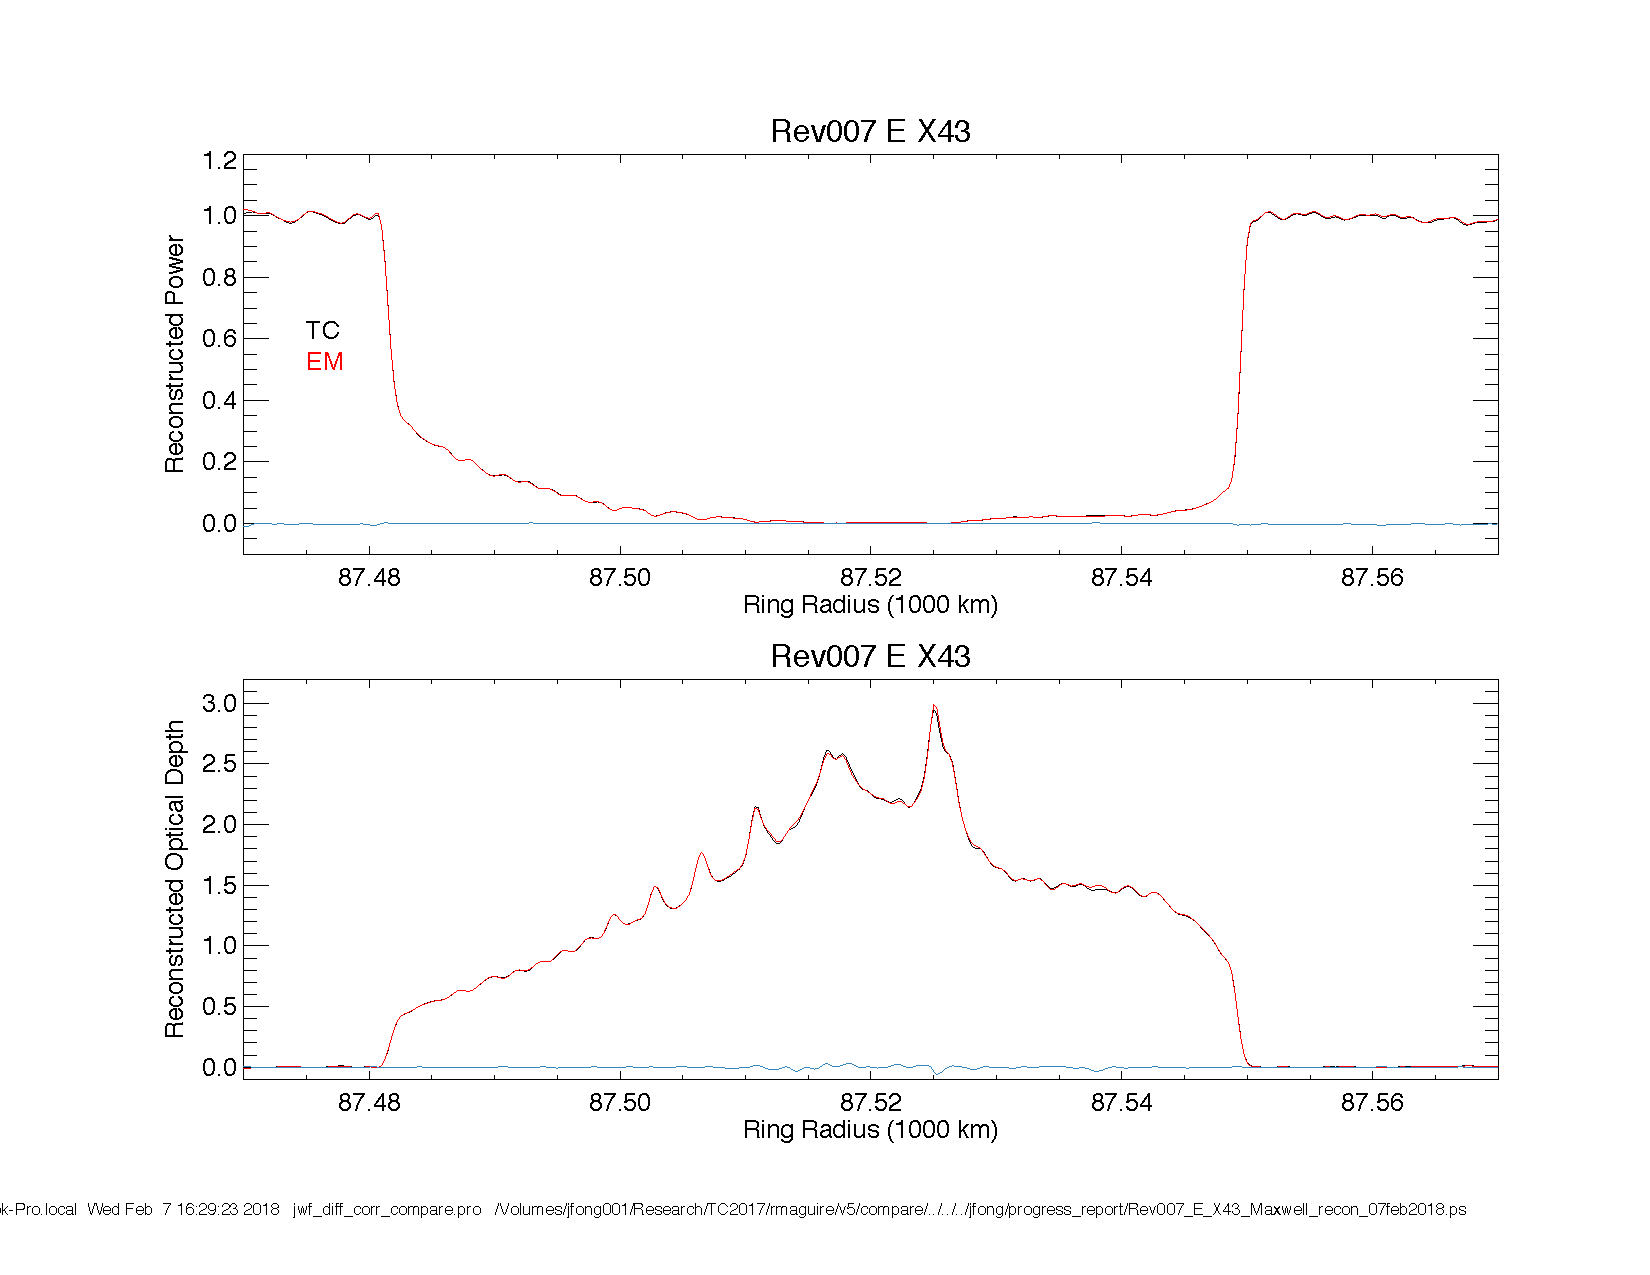
\includegraphics[page=1,trim = {0.67in 0.5in 0.5in 0.5in},clip,width=0.8\textwidth]{Rev007_E_X43_Maxwell_recon_07feb2018.pdf}
    \vspace{-4ex}
    \caption[Maxwell Ringlet reconstruction]{A comparison of the diffraction-corrected power (top) and optical depth (bottom) profiles of the Maxwell ringlet for Rev007E X43 from the PDS as produced by Essam Marouf (MC: red) and from our independent analysis (TC:black). The PDS results are plotted in red, and our results are plotted in black. Also shown in each panel is the difference between the PDS and our calculations. The overall agreement is excellent.}
    \label{fig:Maxwell Reconstruction}
\end{figure}
\vspace{-4ex}
\subsubsection{Open Issues}
Overall, we can reproduce the existing \gls{rss} processed data files on the \gls{pds} extremely well, but to achieve this level of agreement for the 1-km resolution profiles we had to scale the assumed radial resolution by a factor of almost exactly $1/\sqrt{2}\approx0.7071$, compared to the definition of $\Delta R$ given in MTR86. We have no explanation for this discrepancy, but for all results in this report, we consistently apply a $1/\sqrt{2}$ factor to the specified resolution of data on the \gls{pds}. We also note that our ability to compare the details of our calculations with those on the \gls{pds} is limited by the absence of the normalized diffraction pattern as a function of uniform radius, just prior to the diffraction reconstruction step. 
\subsection{Additional Tests}
Although the \gls{pds} does not provide calibrated diffraction patterns, which would enable users to compare their own calibrations and \gls{diffraction reconstruction} methods with the archived results, we have in hand some files provided by \gls{rss} team member Essam Marouf with reconstructed optical depth profiles that are similar (but not identical) to those on the \gls{pds}, which additionally include the calibrated diffraction patterns prior to the Fresnel inversion step. In this section, we use our processing code to compare both our normalized diffraction patterns and our final reconstructed optical depth profiles with Marouf's. Then, as a test of our ability to produce high-resolution ring profiles under demanding geometric conditions, we show preliminary high-resolution diffraction-corrected \gls{f ring} profiles on Rev 123E at \glslink{s-band}{S}, \glslink{x-band}{X}, and \glspl{ka-band}.
\subsubsection{C Ring Ripples - Rev133E}
\label{subsubsec:C_ring_ripples}
The Rev133E RSS ring \gls{occultation} probed Saturn's rings at a very small \gls{ring opening} angle, greatly enhancing the sensitivity to small changes in apparent \gls{optical depth} and to slight inclinations in the orbits of ring material. As reported by \citealt{Marouf2011}, quasi-periodic structure was observed in the inner \gls{c ring}, having the appearance of two co-added sinusoidal signals of slightly different radial wavelengths. One interpretation of these observations is that the rings suffered two collisions several hundred years ago, resulting in very slight inclinations of the rings that then differentially precessed about the node, producing a corrugated vertical ripple pattern in the rings. Figure \ref{fig:CringRipples} shows the optical depth profile of this region, along with simple models that attempt to reproduce the beating between the two sinusoidal signals.
\begin{figure}[H]
    \centering
    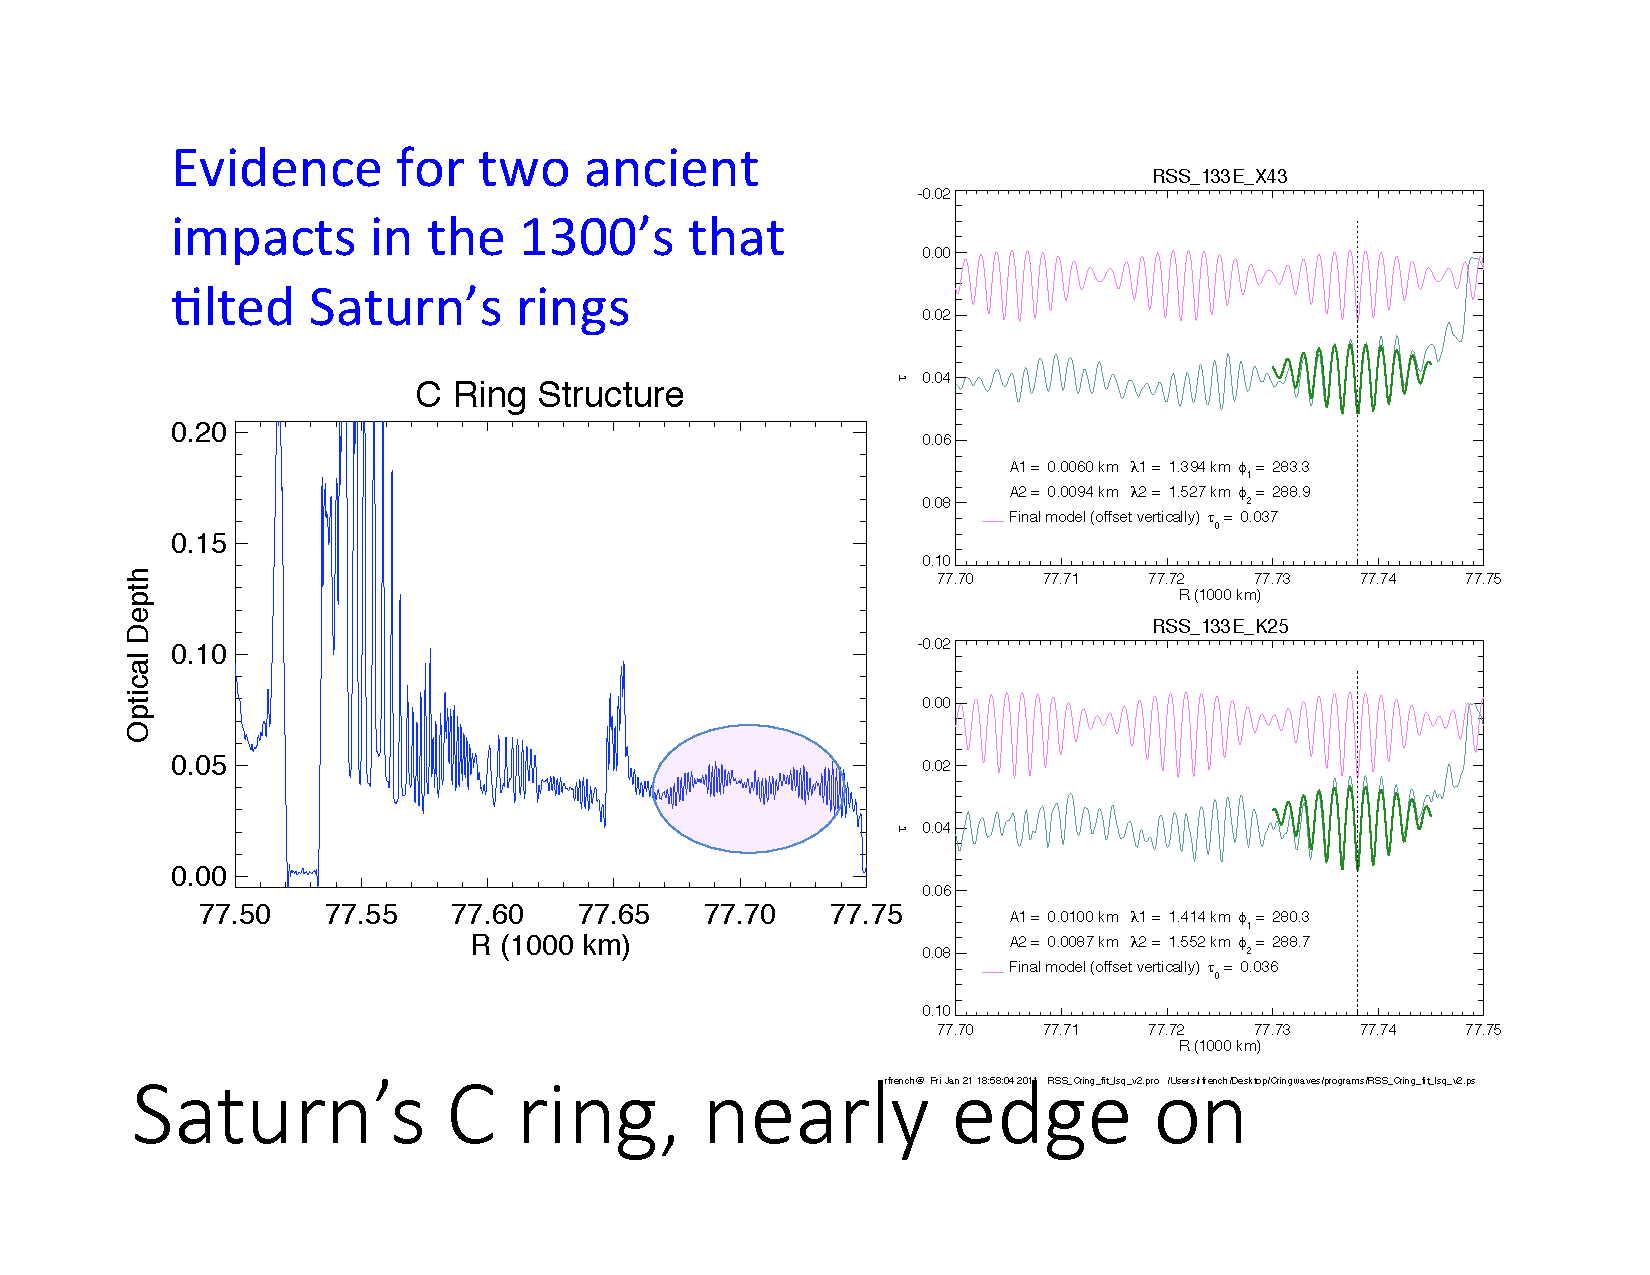
\includegraphics[page = 1,trim = {0.8in 1.5in 1.0in 1.0in},clip,width=0.7\textwidth]{CringRipples.pdf}
    \caption[C ring ripples]{Rippled structure in the inner C ring, modeled as differentially precessing structures. The green curves at right show high-resolution radial structure obtained by diffraction correction of the X-band (upper panel) and Ka-band (lower panel) observations.}
\label{fig:CringRipples}
\end{figure}
Although these data have not been archived to the \gls{pds}, they represent the highest resolution reconstructions we have in hand from Essam Marouf, and provide a critical test of our ability to perform diffraction corrections to low-inclination ring occultations at sub-km resolution. We first compare our derived normalized and phase-corrected diffraction patterns with Marouf's. Figure \ref{fig:CringRipplesDiffraction} shows the normalized power and phase of the diffraction pattern for the X43 and Ka25 observations, at 250 m and 200 m resolution, respectively. The black curve shows Marouf's results, our results are shown in red, and the differences are shown in blue. There is a slow drift of the retrieved phase and an accumulated DC phase offset (not shown) that result from slightly different residual frequency corrections between the two analyses. Overall, the agreement in both normalized power and phase is quite good, especially for the Ka-band, confirming our ability to match the Marouf retrieved optical depth profiles to a high degree of fidelity.\par
Next, we use Marouf's diffraction pattern as input for our Fresnel inversion code, and compare our retrieved optical depth profiles with Marouf's, using identical inputs. For this test, we adjusted our assumed radial resolution to provide the best match to Marouf's derived optical depth profiles. As we noted above, we find that we need to assume a processing resolution of roughly $1/\sqrt{2}$ times that defined by MTR86 in order to give the best match to Marouf's reconstructions at his stated resolution.\par
\begin{figure}[htbp]
    \centering
    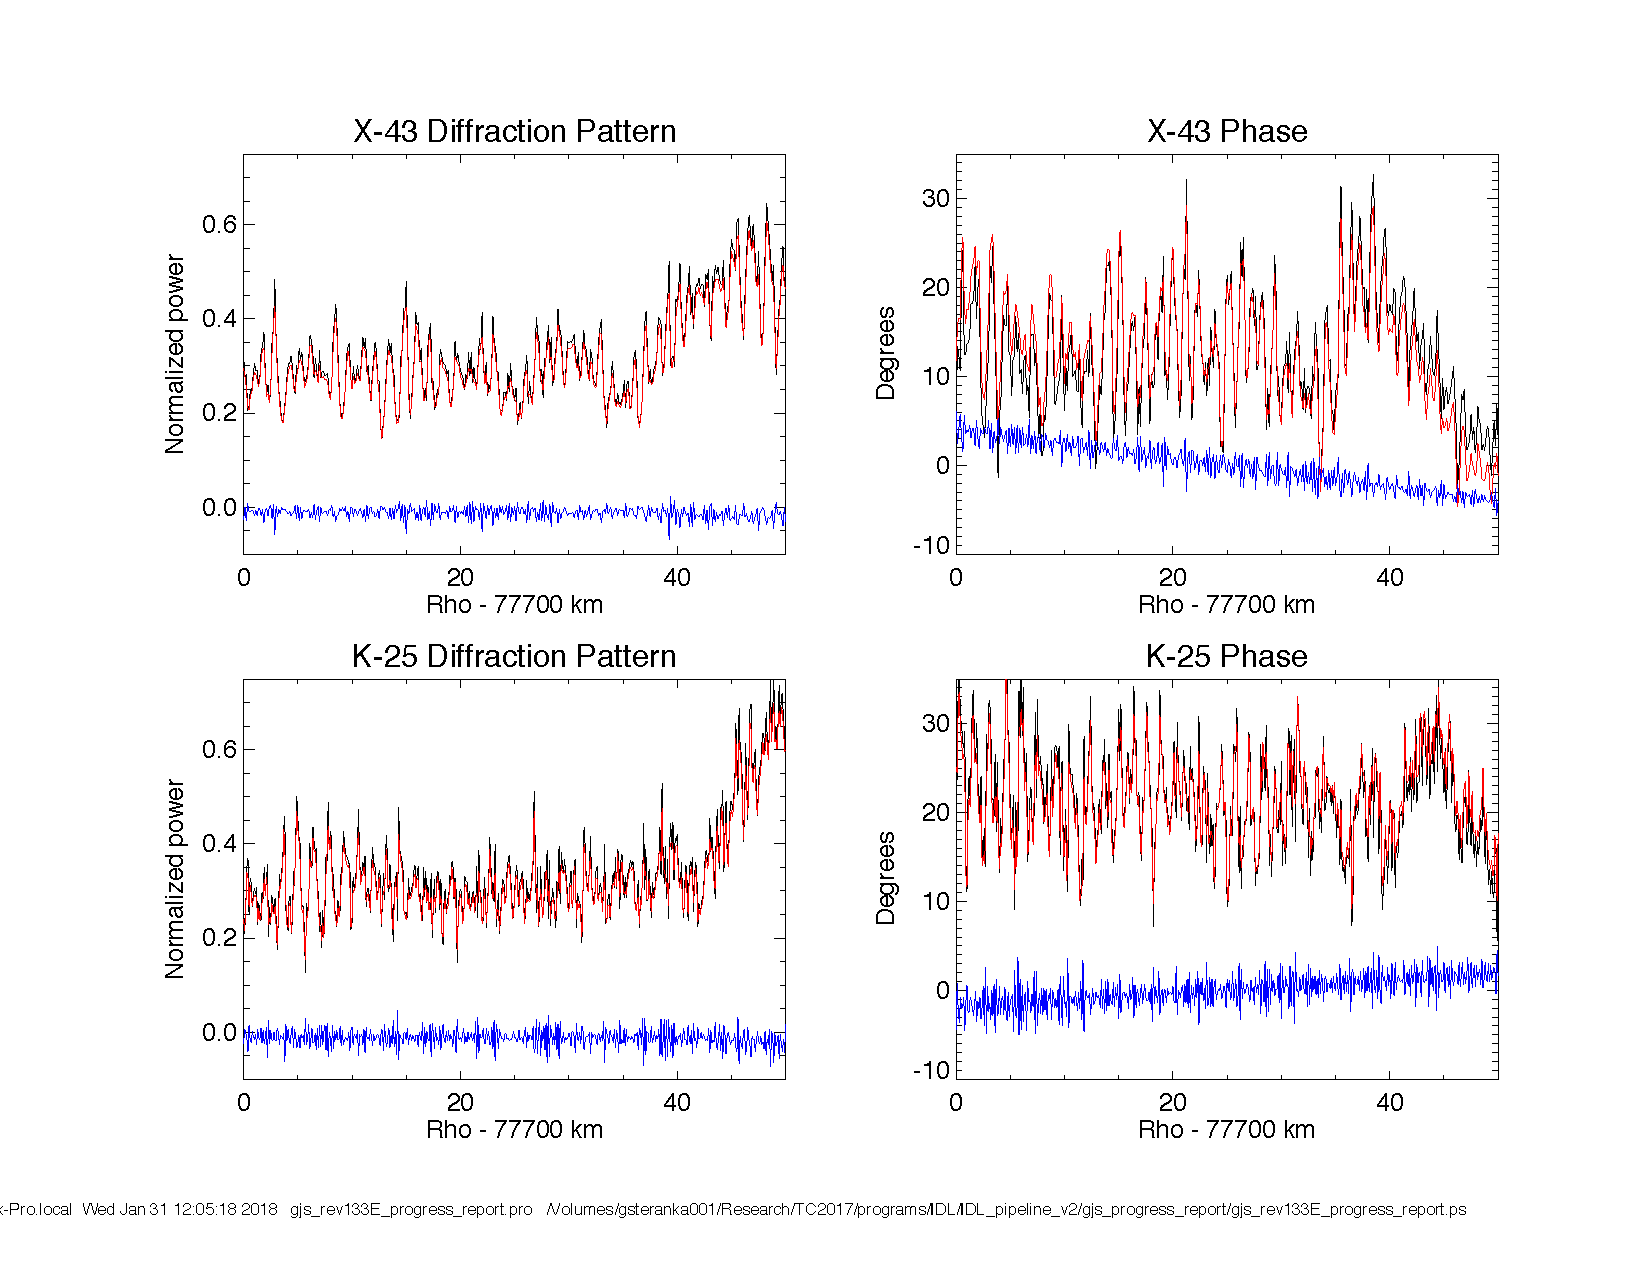
\includegraphics[trim = {1.0in 0.5in 1.0in 0.75in},clip,width=0.7\textwidth]{CringRipplesDiffraction.pdf}
    \caption[Comparison of C ring diffraction patterns]{Diffraction pattern of the Rev133E RSS occultation over a 50-km range of the central C ring, at X- (upper panels) and Ka25-bands (lower panels) normalized power (left) and frequency-corrected phase (right), as obtained by Marouf (black) and by our group (red). Also shown (offset, and in blue) are the differences between the two sets of results. }
    \label{fig:CringRipplesDiffraction}
\end{figure}
\begin{figure}[htbp]
    \centering
    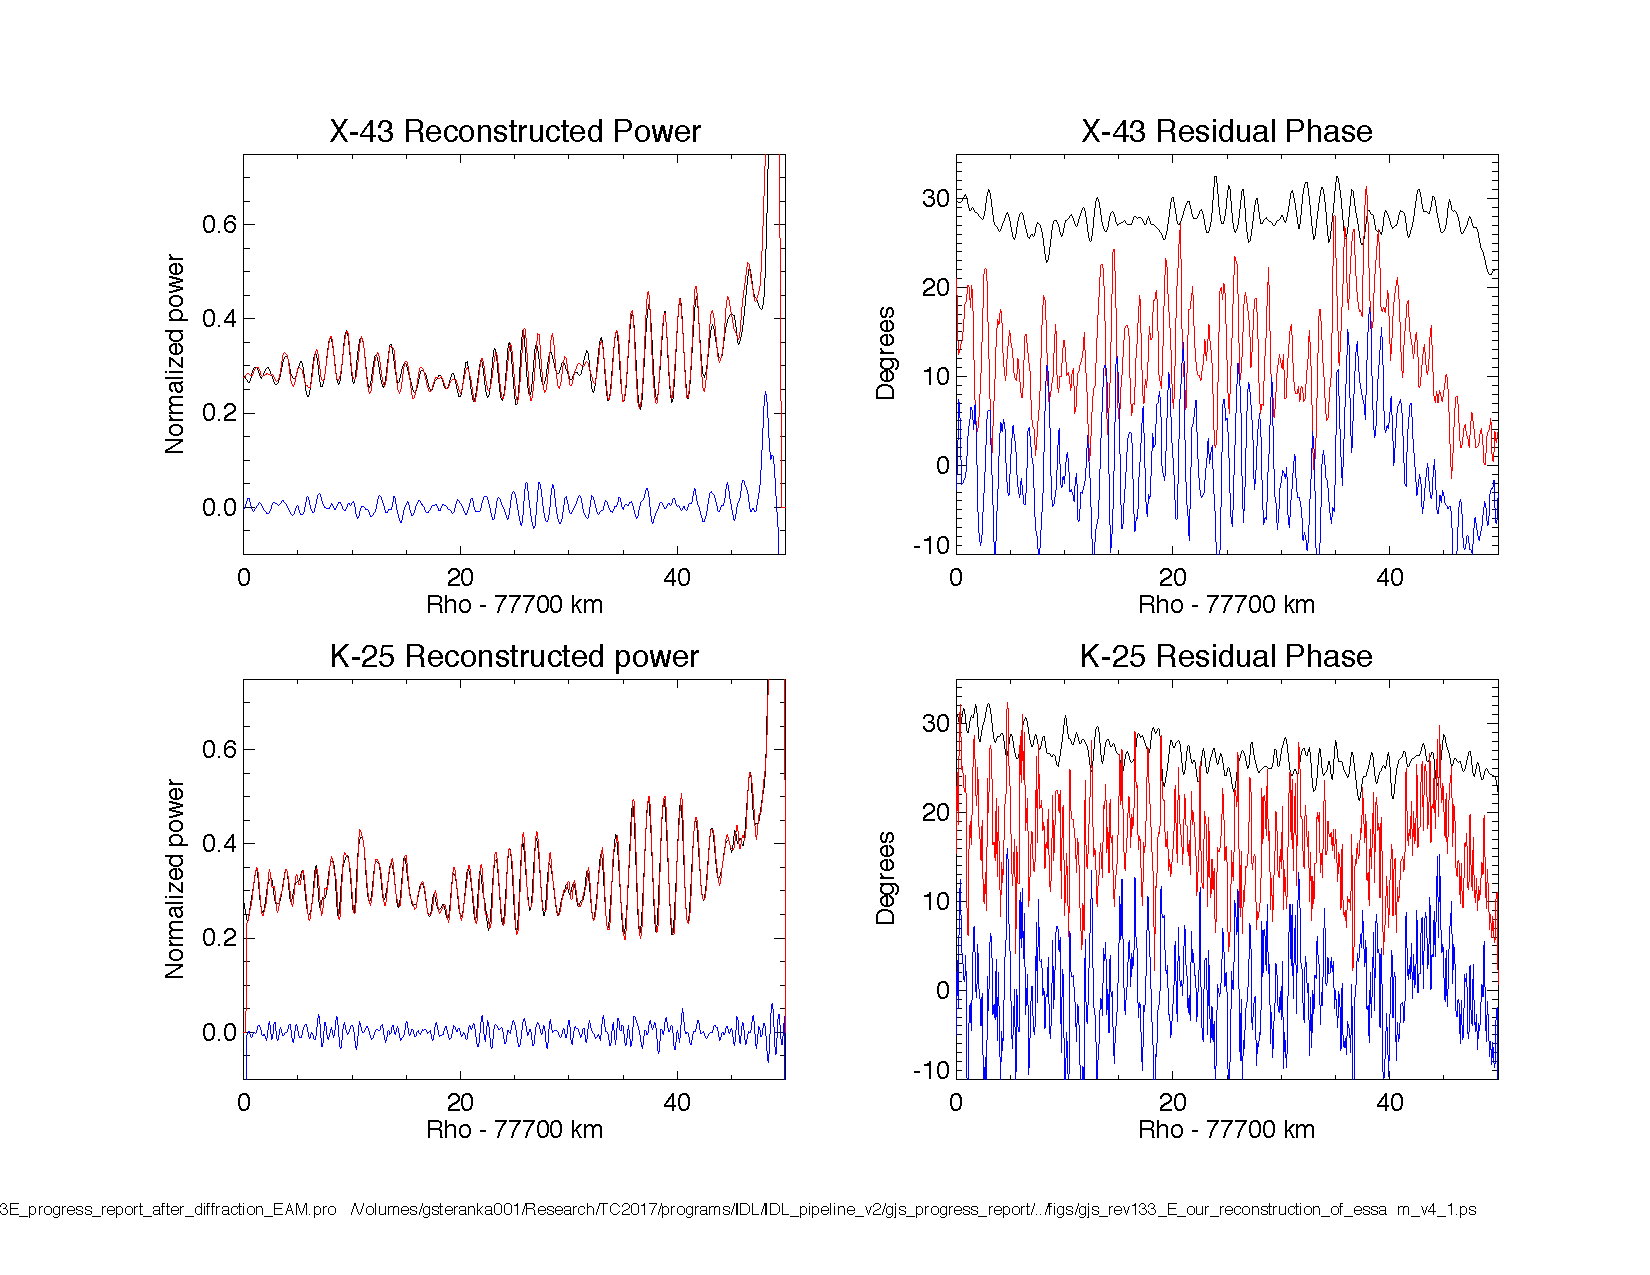
\includegraphics[trim = {1.0in 0.5in 1.0in 0.75in},clip,width=0.7\textwidth]{CringRipplesTau2.pdf}
    \caption[Comparison of C ring optical depth profiles] {Comparison of the Rev133E X43 (upper panels) and Ka25 (lower panels) reconstructed optical depth (left) and residual phase (right) profiles, as obtained by Marouf (black) and by our group (red), using as input Marouf's normalized diffraction results. Also shown (offset, and in blue) are the differences between the two sets of results. The reconstructed power curves are generally in excellent agreement, with the Ka-band results agreeing somewhat better than the X-band results, where the residuals show some lingering systematic rippled structure of unknown origin.}
    \label{fig:CringRipplesTau2}
\end{figure}
\begin{figure}[htbp]
    \centering
    \vspace{-5ex}
    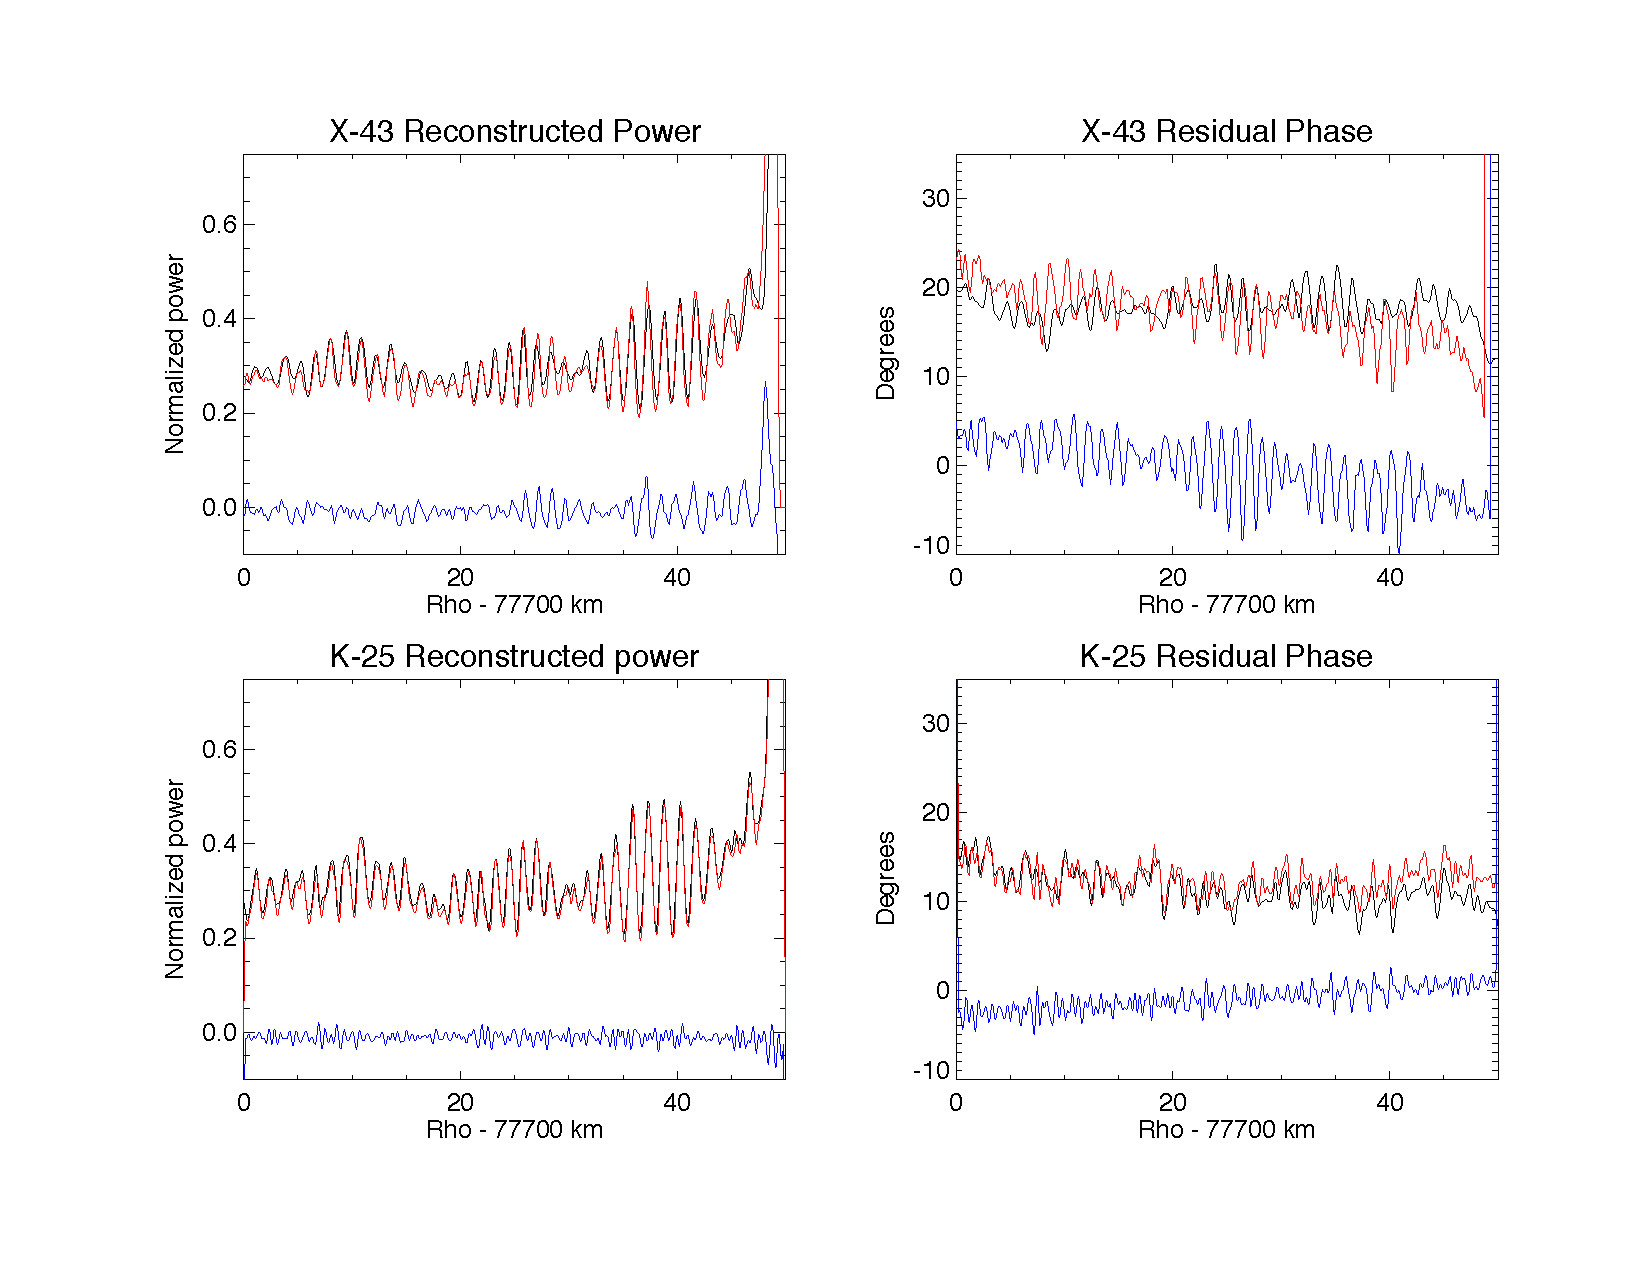
\includegraphics[page = 1,trim = {1.0in 0.5in 1.0in 0.75in},clip,width=0.7\textwidth]{CringRipplesTau.pdf}
    \caption[Comparison of independently-derived C ring optical depth profiles] {Comparison of the Rev133E X43 (upper panels) and Ka25 (lower panels) optical depth (left) and residual phase (right) profiles, based on completely independent analyses by Marouf (black) and by our group (red). Also shown (offset, and in blue) are the differences between the two sets of results.}
    \label{fig:CringRipplesTau}
\end{figure}
The final results are shown in Fig.~\ref{fig:CringRipplesTau2}. The optical depth profiles for both wavelengths match Marouf's very well, demonstrating the ability of our diffraction correction in reproducing Marouf's reconstructed profiles. However, as can be seen, reproducing Marouf's residual phase in detail remains an as-yet unresolved problem. Fortunately, the principal science goal is to determined the diffraction-corrected optical depth, where the agreement is quite good. Nevertheless, we will continue to investigate these discrepancies, which may be attributable to different assumptions in our processing steps that we have are not aware of, given the incomplete documentation of the intermediate results in question. Overall, we regard these tests as quite successful in showing that we can retrieve fine-scale radial structure under demanding geometrical circumstances such as the grazing geometry of this occultation.\par
As a final test, we compare Marouf's derived optical depth profiles with ours when we use our diffraction pattern (Fig.~\ref{fig:CringRipplesDiffraction}) as input to our Fresnel inversion code, rather than Marouf's. The results of these two completely independent analyses are shown in Fig.~\ref{fig:CringRipplesTau}. This test yields a better match to Marouf's residual phase than that in Fig.~\ref{fig:CringRipplesTau2}, particularly for Ka band data. However, the discrepancy in the X band residual phase remains unexplained.
Collectively, these tests demonstrate that our data processing methods can produce diffraction-corrected optical depth profiles at very high resolution that closely match the independent results by Marouf, for the cases we have been able to compare in detail.
\subsection{High Resolution F Ring Profiles}
Current Cassini RSS data on the PDS do not include high-resolution profiles of the F ring, but they are of high scientific interest, and they provide an example of the kinds of structures that our code will make newly accessible to general users. We illustrate the capabilities of our inversion technique by showing preliminary versions of high resolution diffraction-corrected profiles of the F ring retrieved from the Rev 123E occultation at three wavelengths. \par
We begin with the high SNR X-band results. Figure \ref{fig:Fring-X} shows the diffraction pattern (normalized power and phase) as solid black lines in the upper and lower panels, respectively. The red curve in the upper panel shows the retrieved diffraction-corrected profile, revealing a very narrow core. The absence of any residual diffraction artifacts in the retrieved profile is a strong indication that the inversion process has been properly applied. The blue curve stretches the retrieved profile radially by a factor of ten (note the 1 km scale bar) to reveal the shape of the derived optical depth profile at sub-km resolution.
\begin{figure}[htbp]
    \centering
    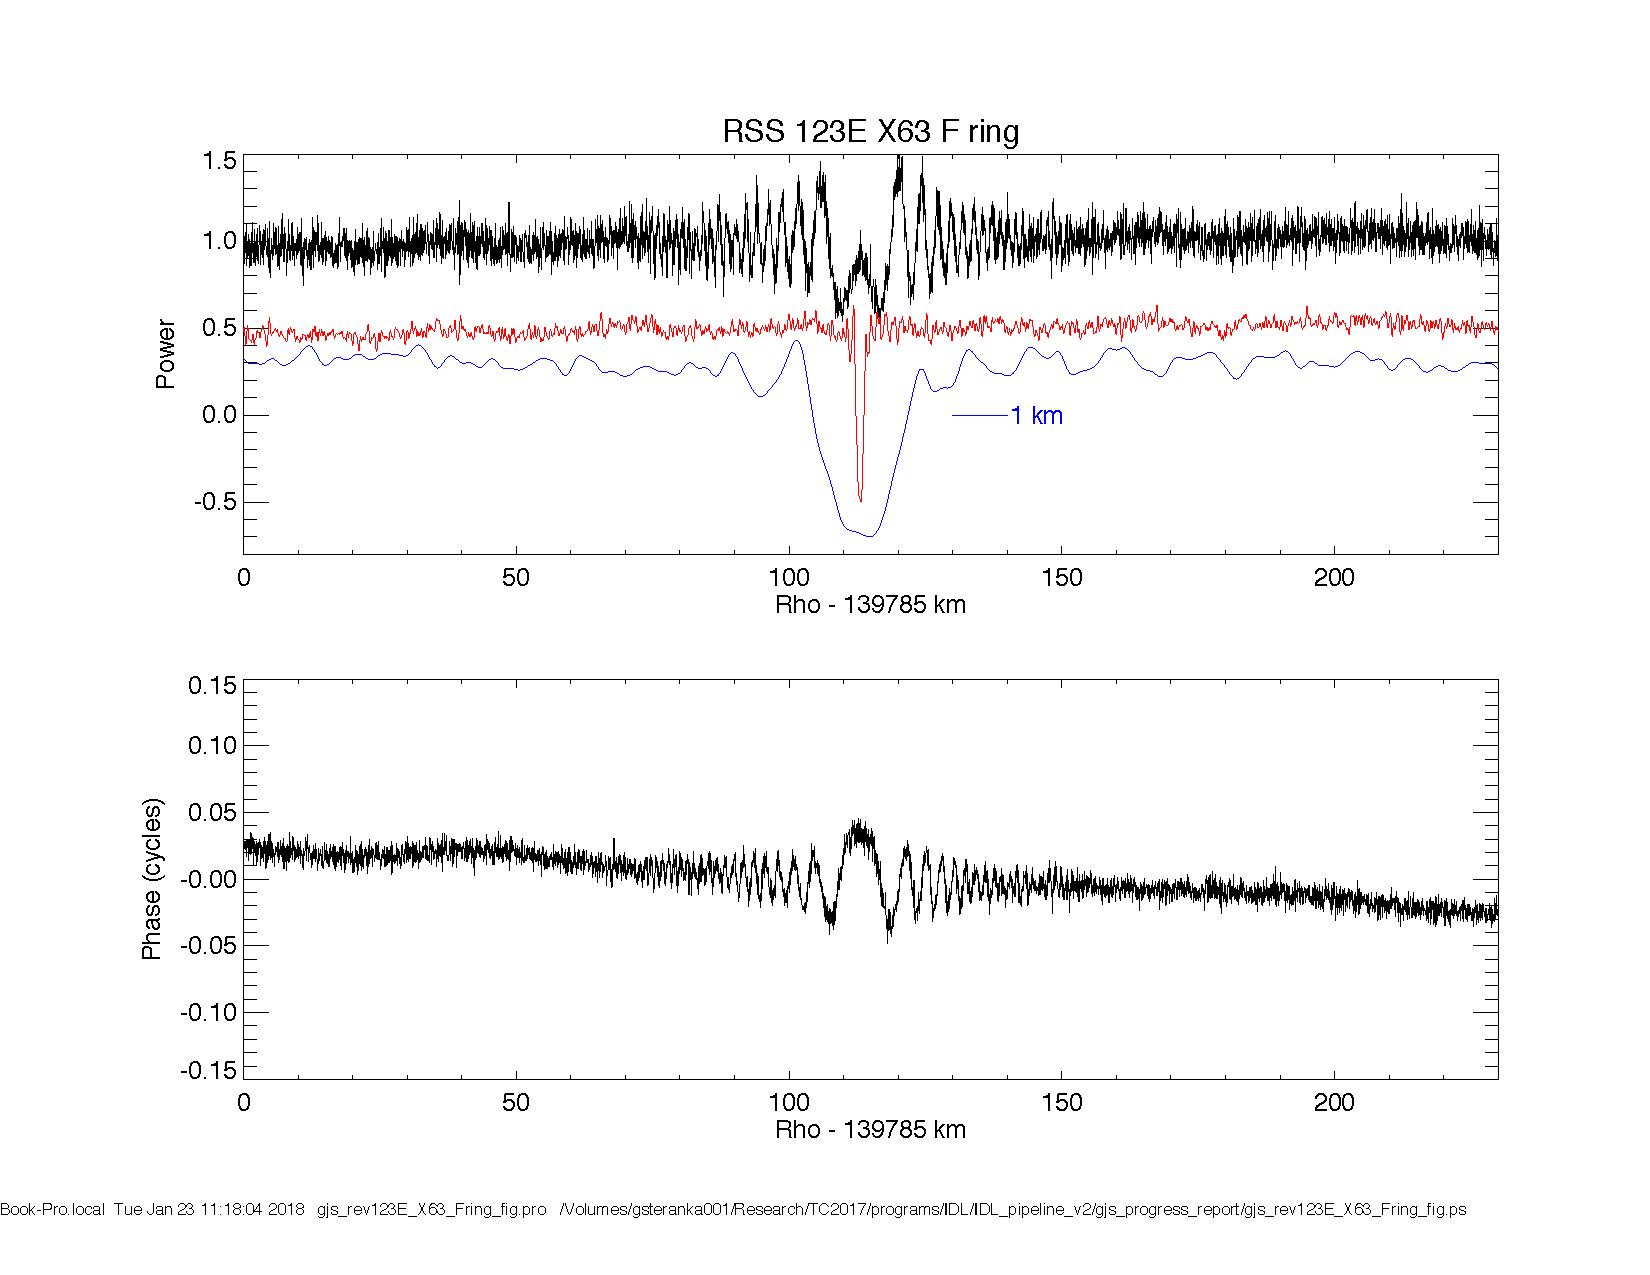
\includegraphics[trim = {0.0in 0.8in 0.0in 0.75in},clip,width=0.9\textwidth]{gjs_rev123E_X63_Fring_fig.pdf}
    \caption[F ring profile - X band] {Diffraction pattern and retrieved radial profile of the F ring as observed at X band during the Rev123E RSS ring occultation.}
    \label{fig:Fring-X}
\end{figure}
Next, we show the corresponding Ka-band results in Fig.~\ref{fig:Fring-Ka}. The radial scale of the plot is the same as in Fig.~\ref{fig:Fring-X}, but the diffraction pattern appears to be compressed because of the shorter wavelength of the Ka-band observations, and thus the shorter characteristic Fresnel scale length of the diffraction fringes. Once again, there is a sub-km narrow core in the retrieved F ring profile.\footnote{The detailed shape of the diffraction-corrected profile differs somewhat from the X-band results, but additional sensitivity studies need to be performed before concluding that these differences are statistically significant.}
\begin{figure}[htbp]
    \centering
    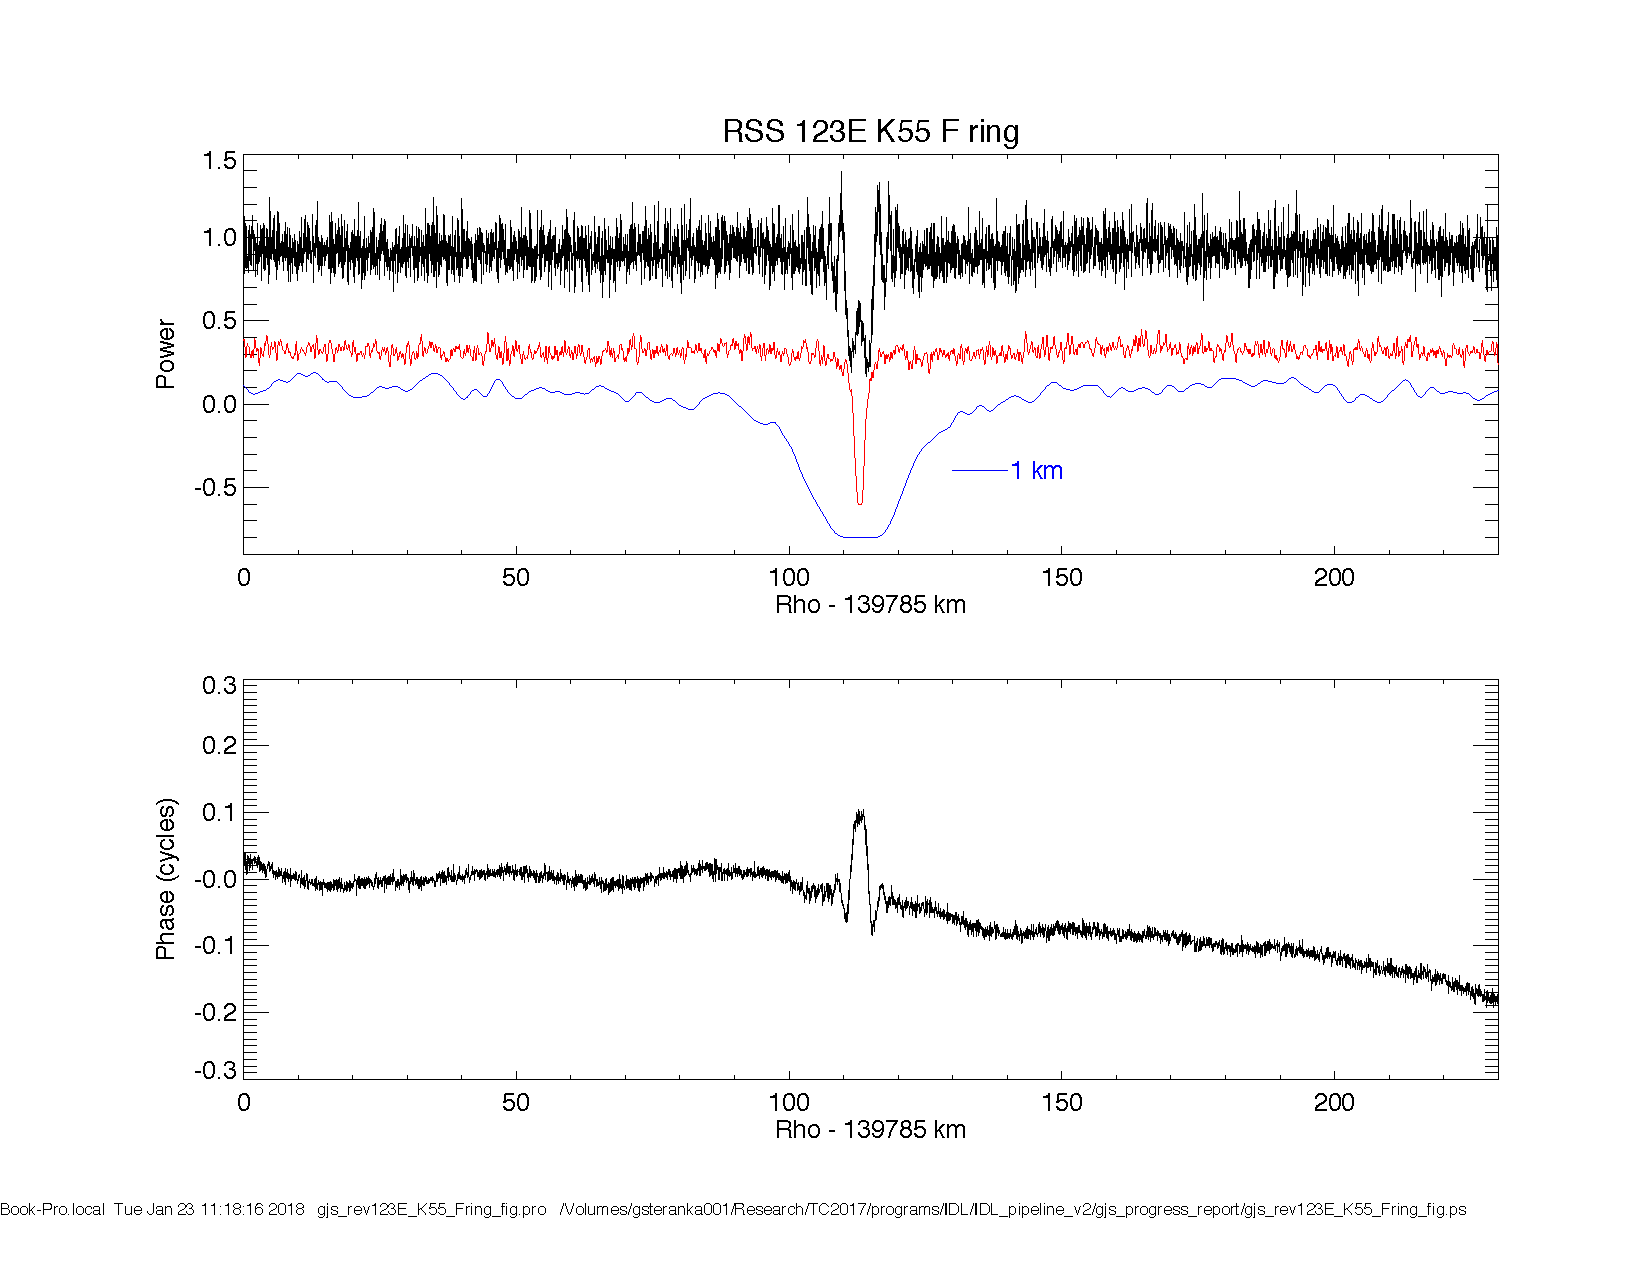
\includegraphics[trim = {0.0in 0.8in 0.0in 0.75in},clip,width=0.9\textwidth]{gjs_rev123E_K55_Fring_fig.pdf}
    \caption[F ring profile - Ka band] {Diffraction pattern and retrieved radial profile of the F ring as observed at Ka band during the Rev123E RSS ring occultation.}
    \label{fig:Fring-Ka}
\end{figure}
Finally, we show the S-band observations of the F ring during Rev 123E in Fig.~\ref{fig:Fring-S}. The diffraction fringes are visible across the entire radial range shown. Although this preliminary retrieved diffraction-corrected F ring profile may be distorted by using an overly-restricted radial range of data, it does show that the F ring is clearly detected at the longest of the RSS wavelengths, indicating the presence of significant decimeter-sized particles in the core of the F ring.
\begin{figure}[H]
    \centering
    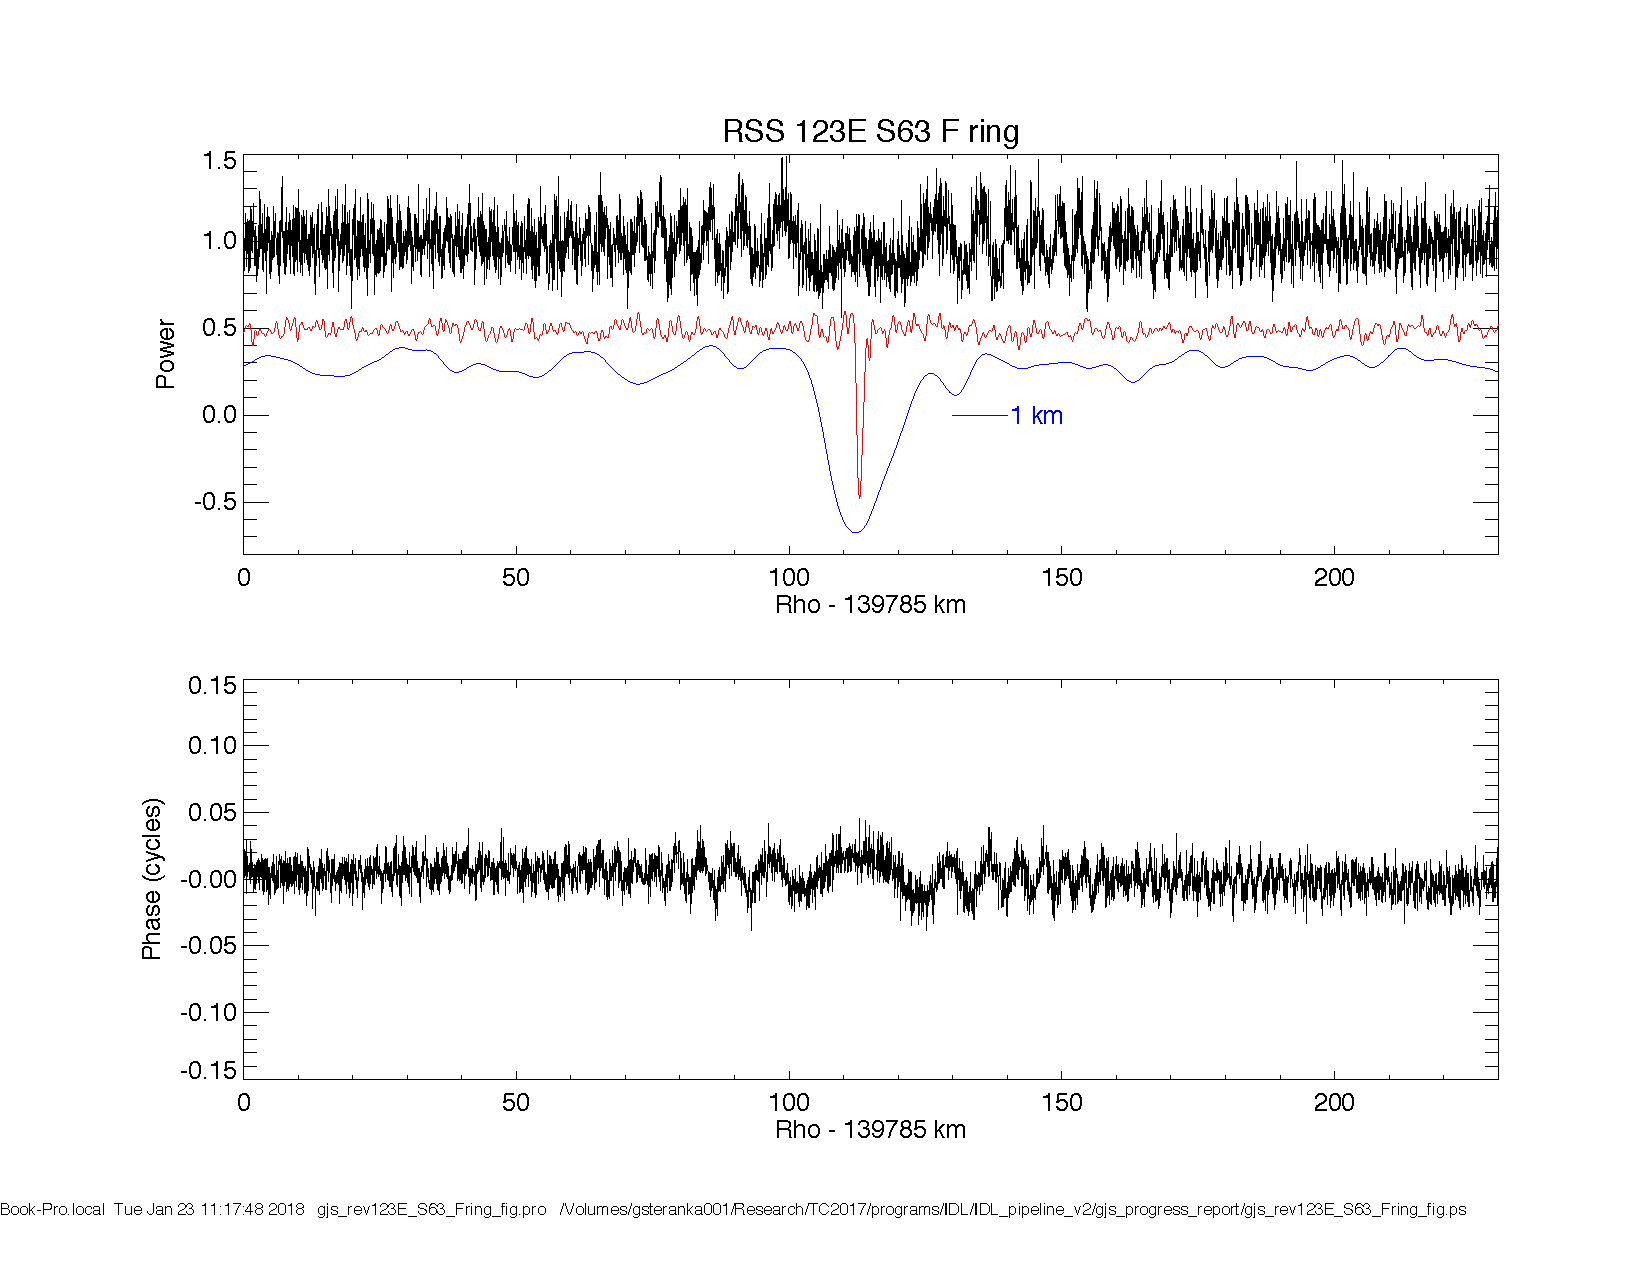
\includegraphics[trim = {0.0in 0.8in 0.0in 0.75in},clip,width=0.9\textwidth]{gjs_rev123E_S63_Fring_fig.pdf}
    \caption[F ring profile - S band] {Diffraction pattern and retrieved radial profile of the F ring as observed at S band during the Rev123E RSS ring occultation.}
    \label{fig:Fring-S}
\end{figure}
\section{Proposed PDS Organization and Contents}
\label{section:proposed pds organization and contents}
As part of our proof of concept for our processing pipeline, we will submit a separate volume ({\tt CORSS\_8101}) to the PDS that contains reconstructed radial profiles of representative RSS ring occultations at 0.5 and 1.0 km resolution at S-, X- and K-band, from the inner C ring to beyond the F ring. Ultimately, this volume will contain a substantial fraction of available RSS observations (prior to the USO failure), with the final contents dependent on the time available for producing reliable and well-documented results. 
\subsection{Directory Structure}
For consistency with existing archived Cassini RSS ring profiles, our proposed directory structure closely resembles that already found on the PDS, with augmentations to provide additional overview information and intermediate results. Below, we show the directory structure of an existing PDS volume, {\tt CORSS\_8001}, that includes 1- and 10-km X-band ring profiles from RSS observations between Rev007 (May 2005) and Rev067 (May 2008):
\lstset{
  basicstyle=\footnotesize\ttfamily,
  columns=fullflexible,
  keepspaces=true,
  framexleftmargin=4pt,
  frame = single,
  escapechar="}
\begin{lstlisting}[linebackgroundcolor={
\ifnum\value{lstnumber}=18\color{pink}\fi
\ifnum\value{lstnumber}=19\color{pink}\fi
\ifnum\value{lstnumber}=20\color{pink}\fi}]
CORSS_8001
|
|-AAREADME.TXT..........This file.
|-ERRATA.TXT............A file that reports any known errors and describes any known
|                       deviations from PDS standards.
|-VOLDESC.CAT...........A PDS volume object, providing a high-level
|                       description of the volume and its contents.
|-EASYDATA..............Directory containing ring occultation profiles in ASCII tables.
| |
| |- RevXX..............A directory containing data and support files for an occultation.
| | |-XX_CAL.TAB........A calibration file for the corresponding ring profile (*_TAU).
| | |-XX_CAL.LBL........Detached PDS labels for the above.
| | |-XX_GEO.TAB........A geometry file for the corresponding ring profile (*_TAU).
| | |-XX_GEO.LBL........Detached PDS labels for the above.
| | |-XX_TAU.TAB........A ring radial profile from a single occultation, ingress and
| | |                   egress portions are given in separate files.
| | |-XX_TAU.LBL........Detached PDS labels for the above.
| | |_YY_Summary.PDF....A file containing documentation for the 
| | |                   associated observations. 
| | |_YY_Summary.LBL....Detached PDS labels for the above.
|-CATALOG/..............A directory containing PDS catalog information, providing 
| |                     high-level descriptions of the data, instruments, etc.
| |
| |-CATINFO.TXT.........Description of the files in this directory.
| |-DATASET.CAT.........PDS catalog file describing this data set, including a brief 
| |                     summary of the data and the processing involved.
| |-INST.CAT............Catalog file describing RSS.
| |-INSTHOST.CAT........Catalog file describing Cassini.
| |-MISSION.CAT.........Catalog file describing the observing campaign.
| |-PERSON.CAT..........Catalog file describing the personnel involved in acquiring
| |                     and archiving this data set.
| |-REF.CAT.............Catalog file containing relevant bibliographic references.
|-DOCUMENT/.............A directory containing supplemental documentation.
| |
| |-DOCINFO.TXT.........Description of the files in this directory.
|-INDEX/................A directory containing indices of the files in this data set.
| |
| |-INDXINFO.TXT........Description of the files in this directory.
| |-INDEX.TAB...........A table of all the data files on this volume.
| |-INDEX.LBL           A detached PDS label, defining each column in the table.
\end{lstlisting}  
We will submit our reproduction of {\tt CORSS\_8001/EASYDATA/Rev07E\_RSS\_2005\_123\_X43\_E} and associated summary, geometry, and calibration files along with this interim report.

This is the proposed directory structure for {\tt CORSS\_8101}:
\begin{lstlisting}[linebackgroundcolor={
\ifnum\value{lstnumber}=4\color{yellow}\fi
\ifnum\value{lstnumber}=30\color{yellow}\fi
\ifnum\value{lstnumber}=31\color{yellow}\fi
\ifnum\value{lstnumber}=35\color{yellow}\fi
\ifnum\value{lstnumber}=43\color{yellow}\fi
\ifnum\value{lstnumber}=48\color{yellow}\fi
\ifnum\value{lstnumber}=49\color{yellow}\fi
\ifnum\value{lstnumber}=50\color{yellow}\fi}]
CORSS_8101/.....................Root directory
|
|-AAREADME.TXT..................Text file containing directory structure information.
|-BROWSE/.......................Directory containing auxiliary information.
| |-BROWSE_INFO.TXT.............Description of files in BROWSE/ directory
| |-OVERVIEW/...................Directory containing plots over entire mission: 2005-2017
| | |-B_OVER_MISSION.PDF........Plot of ring opening angle "(Fig.\subref{fig:Bdeg})"
| | |-EARTH_VIEW_MISSION.PDF....Gallery plot of occultation geometry as seen from Earth
| |-YYYY_DOY_Rev###/............Directory containing plots for a single occultation
| | |-OCCULTATION_TRACKS.PDF....Plot of occultation tracks as seen from
| | |                           looking down on the ring plane.
| | |-CIMS_XX.PDF...............Cassini Information Management Systems
| | |                           request display for specific experiment.
| | |-EARTH_VIEW_GEOM.PDF.......Occultation geometry plots as seen from Earth "(Fig.\subref{fig:EarthView})"
| | |-ELEVATION_PLOT.PDF........Plot of the elevation of Cassini above
| | |                           the horizon, from a specific DSN station "(Fig.\subref{fig:Elevation})".
| | |-TAU_PROFILE.PDF...........Plot of ring radial profile.
|-DATA/.........................Directory containing ring occultation profiles
| |                             and 1-kHz RSR files (not currently available on the PDS).
| |
| |-DATA_INFO.TXT...............Description of the files in DATA/ directory.
| |-EASYDATA/...................Directory containing ring occultation
| | |                           profiles in ASCII table files.
| | |-YYYY_DOY_Rev###/..........Directory containing the data and support
| | | |                         files for a single occultation experiment.
| | | |-XX_GEO.TAB..............Geometry file for corresponding ring profile.
| | | |-XX_GEO.LBL..............Detached PDS label for XX_GEO.TAB
| | | |-XX_CAL.TAB..............Calibration file for corresponding ring profile.
| | | |-XX_CAL.LBL..............Detached PDS label for XX_CAL.TAB
| | | |-XX_OBS.TAB..............Observation file for corresponding ring profile.
| | | |-XX_OBS.LBL..............Detached PDS label for XX_OBS.TAB
| | | |-XX_TAU.TAB..............A ring radial profile from a single occultation, with
| | | |                         ingress and egress portions given in separate files.
| | | |-XX_TAU.LBL..............Detached PDS label for XX_TAU.TAB
| |-RAW_1KHZ/...................Directory containing 1-kHz RSR files for all events.
| | |-YYYY_DOY_Rev###/..........Directory containing 1-kHz RSR files for a
| | | |                         single occultation experiment.
| | | |-RSRFILE.................Radio Science Receiver file
|-DOC/..........................Directory containing supplemental documentation.
| |
| |-DOC_INFO.TXT................Description of the files in DOC/ directory.
| |-CASSINI_RSS_USER_GUIDE.PDF..Cassini Radio Science User's Guide (CRSUG).
| |-CASSINI_RSS_USER_MANUAL.PDF.In-depth and extended version of the CRSUG.
|-INDEX/........................Directory containing indices of the files and
| |                             file information in this data set.
| |
| |-INDEX_INFO.TXT..............Description of the files in INDEX/ directory.
| |-DATA_CATALOG.CSV............Catalog of all RSS occultation events and
| |                             corresponding information.
| |-DATA_CATALOG.LBL............Detached PDS labels for DATA_CATALOG.CSV
\end{lstlisting}
We have highlighted our proposed modifications to the current volume in  \textbf{\textcolor{Thistle}{pink}} and our proposed additions in \textbf{\textcolor{Dandelion}{yellow}}. Following the recommendations of the PDS Rings Node, we will no longer include an {\tt EASYDATA} summary PDF in our directory, but will instead add a {\tt BROWSE} directory that contains sample auxiliary information for both individual events and the overall mission. This, along with our proposed data catalog of all RSS files, will allow users to navigate easily between all of the ring occultation events.
We have also chosen to include an {\tt *OBS.TAB} file (included in our sample {\tt CORSS\_8001/EASYDATA/Rev07E\_RSS\_2005\_123\_X43\_E} data set) to document our intermediate steps. This file will include arrays of all input variables (including the normalized observed diffraction patter) required for diffraction-reconstruction step. Also, for users interested in the theory and algorithms behind our ring profile reconstructions, we will provide a Users Manual that will serve as an in-depth and extended version of the CRSUG.
\subsection{Sample Auxiliary Information}
\begin{figure}[htbp]
    \centering
    \begin{subfigure}[t]{0.49\textwidth}
        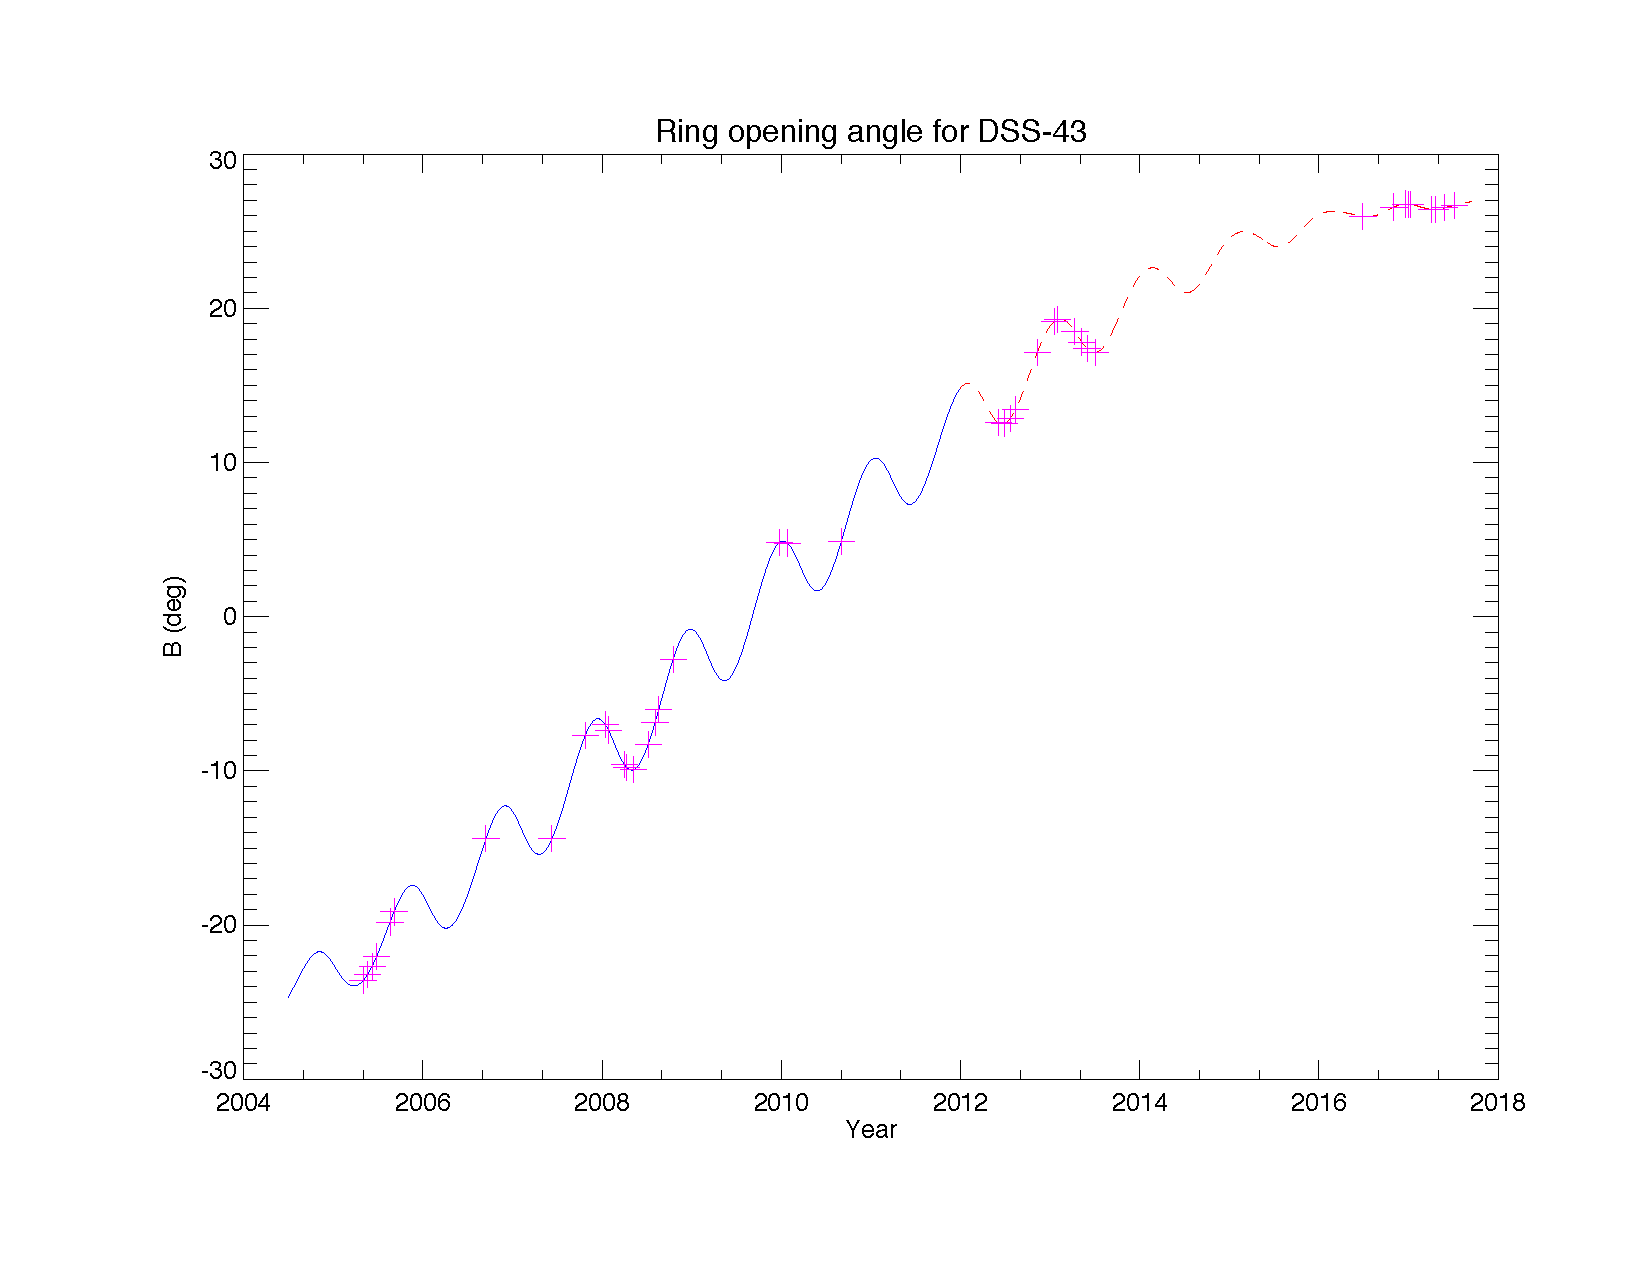
\includegraphics[trim = {0.5in 0.8in 0.5in 0.5in},clip,width=\textwidth]{b_year_dss43.pdf}
        \caption[Ring opening angle vs. year]{Ring Opening angle $(B)$ vs. Time.}
        \label{fig:Bdeg}
    \end{subfigure}
    \begin{subfigure}[t]{0.49\textwidth}
        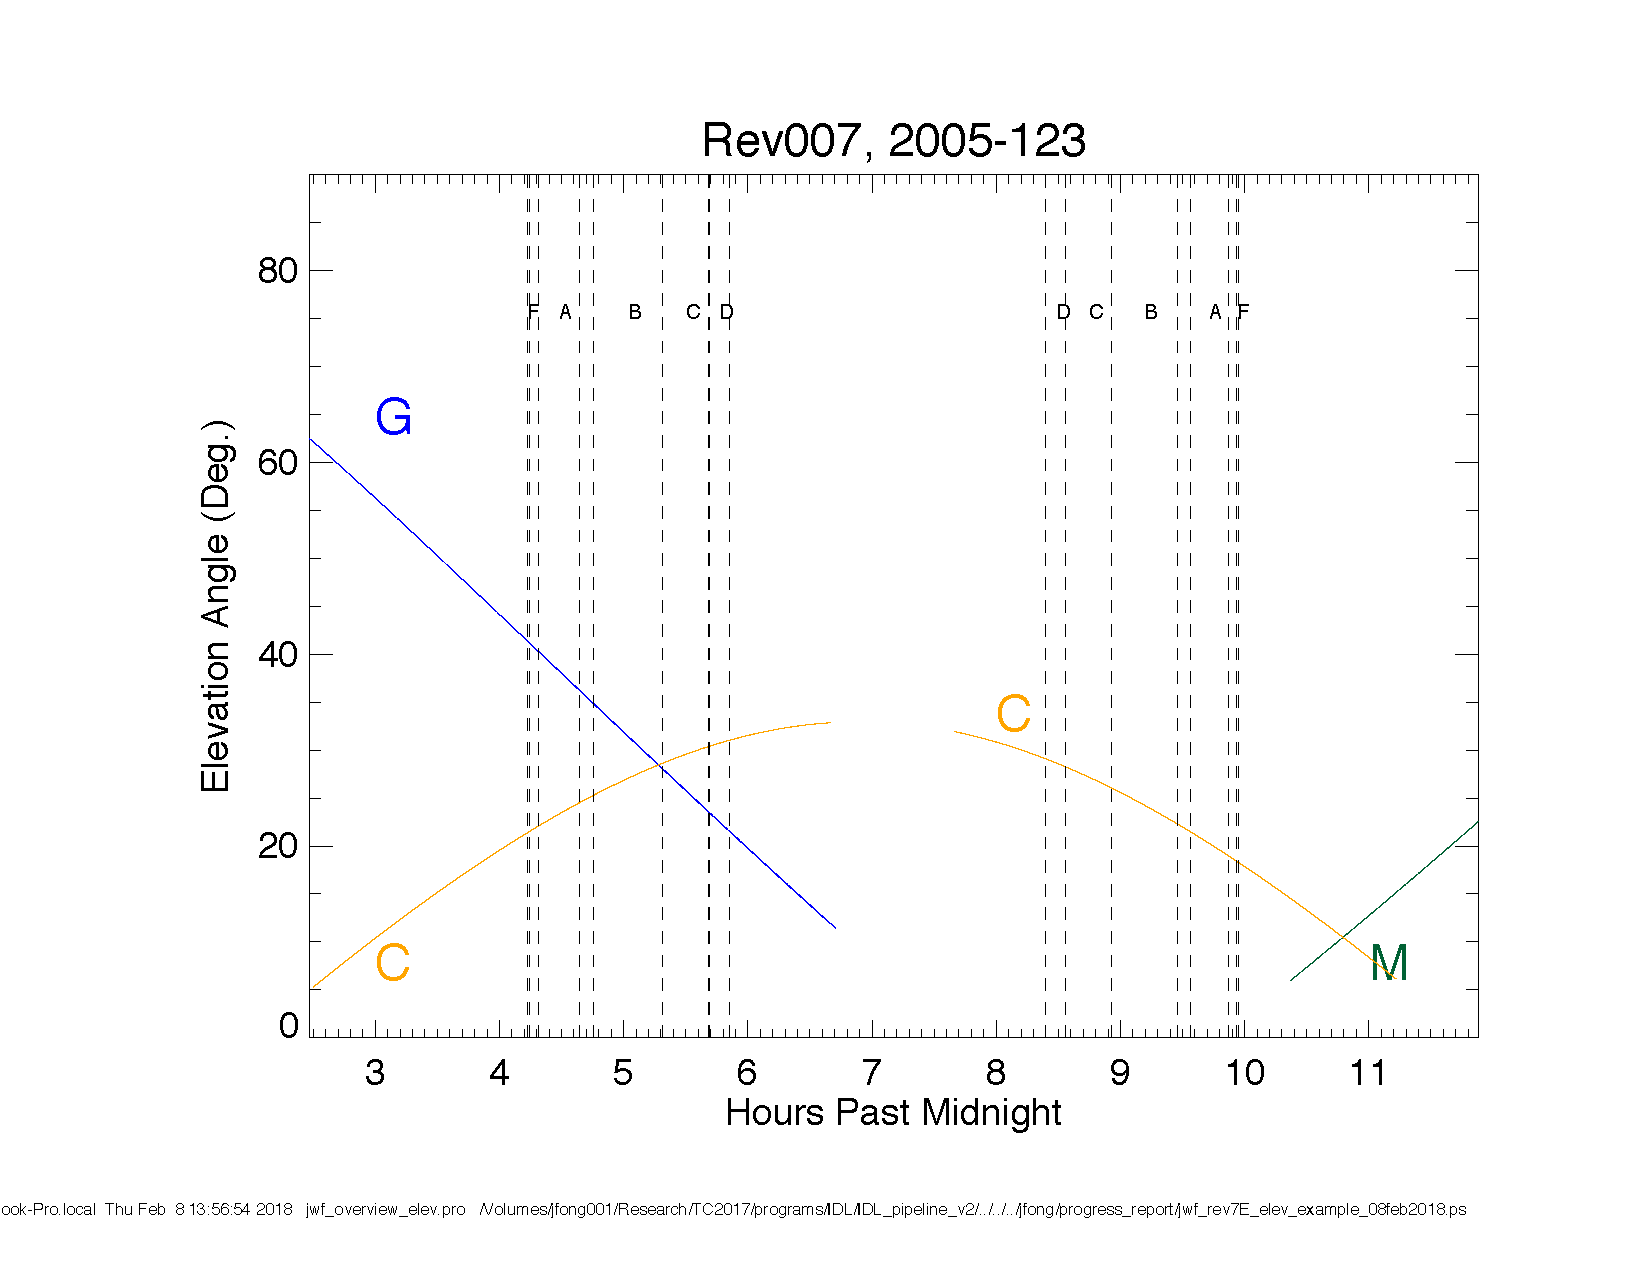
\includegraphics[trim = {0.7in 1.0in 0.7in 0.8in},clip,width=\textwidth]{jwf_rev7E_elev_example_08feb2018.pdf}
        \caption[Elevation plot]{Elevation Plot as a function of time.}
        \label{fig:Elevation}
    \end{subfigure}
    \begin{subfigure}[b]{\textwidth}
        \vspace{0.3in}
        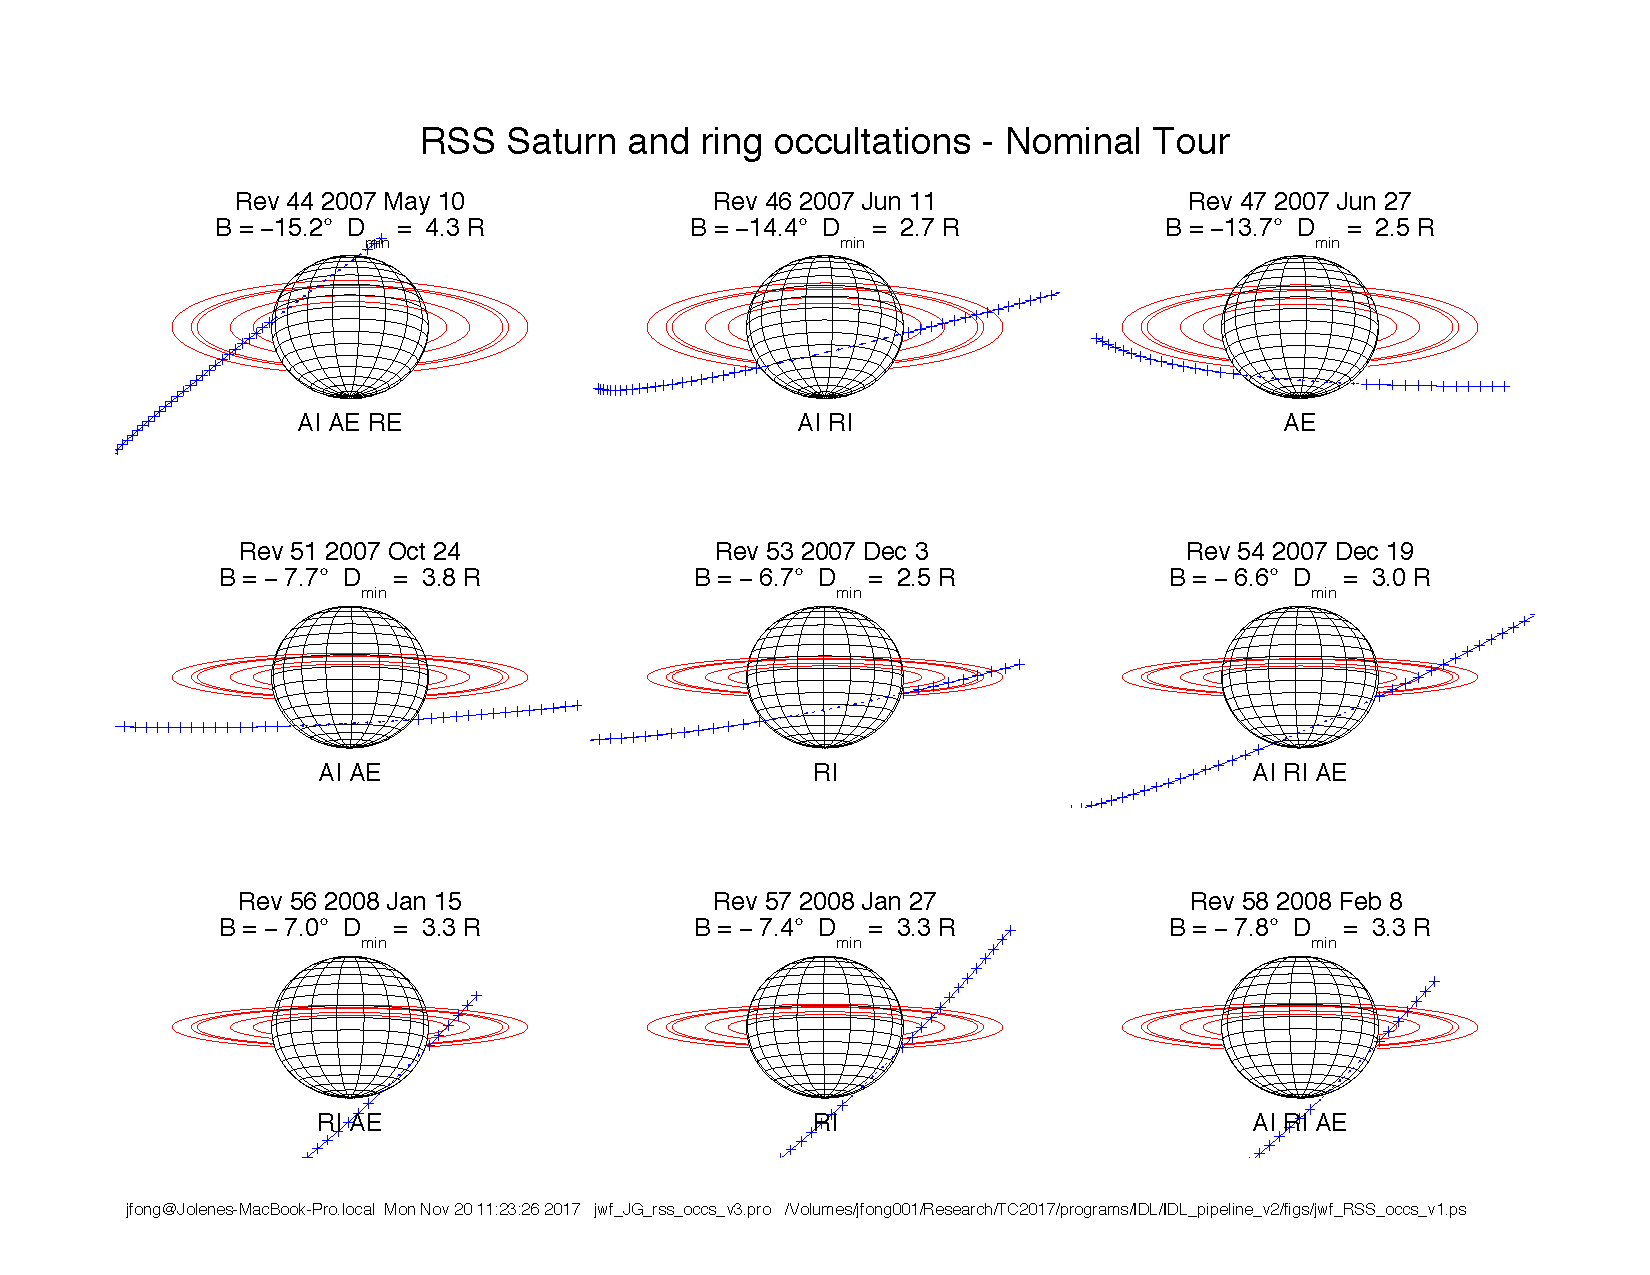
\includegraphics[trim = {0.0in 0.7in 0.0in 0.75in},clip,width=\textwidth]{jwf_RSS_occs_v1_page1.pdf}
        \caption[Earth view of RSS occultations]{Gallery plot showing the Earth view of Saturn and the Cassini spacecraft trajectory, for several of the early ring and atmosphere RSS occultations of the mission.}
        \label{fig:EarthView}
    \end{subfigure}
    \caption[Auxiliary geometry plots]{Fig.~\subref{fig:Bdeg}: An overview of the ring opening angle as viewed from Earth, over the course of the Cassini mission, with individual RSS occultations marked. The dashed curve begins at the time of the RSS USO failure in 2012, after which ring occultations were conducted in two-way mode. Fig.~\subref{fig:Elevation}: Elevation of Cassini spacecraft above the horizon over the course of the Rev007 occultation, as seen from DSN complexes in Goldstone (G), Canberra (C), and Madrid (M). Fig. ~\subref{fig:EarthView}: Earth-based view of a few early occultations.}
    \label{fig:Figures}
\end{figure}
We will provide additional information about the circumstances of the full set of RSS occultations over the Cassini mission. For example, we will include a table containing, for each occultation: the DSN stations involved, the ring plane radius covered, the available RSR files, the ring opening angle, and the ERT for each data set. We will also include helpful graphical overviews of the geometry of the occultations. For example, Fig.~\subref{fig:Bdeg} shows the ring opening angle vs time, between Saturn Orbital Insertion and the End of Mission. Since tenuous regions of the rings (such as parts of the C ring) are more visible at low ring opening angles, while more opaque regions (such as the A and B rings) have higher SNR when the rings are more open, this provides a helpful guide for users about which events might be most appropriate for their specific studies. For each occultation, we will provide a plot of the elevation of the Cassini spacecraft above the horizon as seen form multiple DSN complexes. A preliminary sample elevation plot is shown in Fig.~\subref{fig:Elevation}. Eventually, this will include indications of the times during which ring and atmosphere occultations took place, and the associated RSR files containing data for each ground station.
Additionally, we will include gallery plots of the Earth-based view of the occultations, such as those shown in Fig.~\subref{fig:EarthView}. These are useful for getting an overview of the geometry of individual events, the ring region covered, whether the event is a chord or a more diametric occultation, and whether the planet itself interferes with the ring occultation.
\section{Data Pipeline}
\label{section:data pipeline}
A major goal of this archive project is the production of open-source software and an easy-to-use data pipeline that can be used either to reproduce the full set of processing steps, from raw data to archived results on the PDS, or instead to use existing geometry and calibration files to produce accurate diffraction-corrected profiles for any desired ring region at any specified resolution.
Figure~\ref{fig:gjs_my_label} illustrates the steps of the envisioned data pipeline. 
\begin{figure}[H]
    \centering
    \resizebox{!}{0.8\textheight}{
    \begin{tikzpicture}
        %Nodes
        \begin{scope}[
        roundnode/.style={circle, draw=black, very thick,text width=2em,text centered,fill=green}, squarednode/.style={rectangle,text width=4em,text centered, draw=black, very thick,fill=SkyBlue},bignode/.style={rectangle, draw=black, very thick,text width=4cm,text centered},every edge/.style={draw=black,very thick},bigbig/.style={rectangle, draw=black,thick,text width=5.5cm},every edge/.style={draw=black,very thick},trapanode/.style={trapezium,trapezium left angle=70,trapezium right angle=-70,draw=black,fill=yellow,text width = 3.5cm,text centered},dianode/.style={diamond,draw=black,text width = 3cm, text centered, aspect = 3,inner sep = 0pt,outer sep = 0pt},qnode/.style={circle,draw=black,text width = 8mm,text centered},nonode/.style={circle,draw=black,fill = red,text width = 1cm, text centered, inner sep = 0pt, outer sep = 0pt},yenode/.style={circle,draw=black,fill=SpringGreen,text width = 1cm, text centered,inner sep = 0pt, outer sep = 0pt}]
            \node[cloud,cloud puffs=15.7, cloud ignores aspect, minimum height=2cm, align=center, draw,aspect = 3] (0) {\scriptsize{End-to-End}};
            \node[bignode]      (1)  [below=of 0] {\scriptsize{RSR, Kernels}};
            \node[trapanode]    (2)  [below=of 1] {\scriptsize{Geometry Calculation}};
            \node                    [above left=1mm and 10mm of 2] {\scriptsize{$\{t_{\textrm{OET}}\}$}};
            \node[roundnode]    (3)  [below=of 2] {\scriptsize{*.Geo}};
            \node[trapanode]    (4)  [below=of 3] {\scriptsize{Frequency Extraction}};
            \node                    [above left=1mm and 3mm of 4] {\scriptsize{$\{\Delta t_{freq},t_{s},t_{e}\}$}};
            \node[dianode]      (5)  [below=of 4] {\scriptsize{Plot Frequency Offset}};
            \node[qnode]        (6)  [right=of 5] {\scriptsize{OK?}};
            \node[nonode]       (6n) [above=7mm of 6] {\scriptsize{No}};
            \node[yenode]       (6y) [right=of 6] {\scriptsize{Yes}};
            \node[trapanode]    (7)  [right=of 6y]  {\scriptsize{Frequency Correction}};
            \node[dianode]      (7a) [below=of 7] {\scriptsize{Plot Frequencies}};
            \node[qnode]        (8)  [below=of 7a] {\scriptsize{OK?}};
            \node[nonode]       (8n) [below=of 8] {\scriptsize{No}};
            \node[yenode]       (8y) [left=3.5cm of 8] {\scriptsize{Yes}};
            \node[trapanode] (9) [above=1.5cm of 8y] {\scriptsize{Power Normalization}};
            \node                    [above=1mm of 7] {\scriptsize{$\{\hat{f}_{resid}, \textrm{Fit Order},\textrm{Excluded Zones},\textrm{*.geo}\}$}};
            \node                    [above=1mm of 9] {\scriptsize{$\{\textrm{Spline Order},\textrm{Spline Knots},\textrm{*.geo},\Delta t_P\}$}};
            \node[dianode]      (10)  [below=6mm of 5] {\scriptsize{Plot Power}};
            \node[qnode]        (11) [below=of 10] {\scriptsize{OK?}};
            \node[nonode]       (11n)[right=1cm of 11] {\scriptsize{No}};
            \node[yenode]       (11y)[below=1cm of 11] {\scriptsize{Yes}};
            \node[roundnode]    (12) [below=of 11y] {\scriptsize{*.Cal}};
            \node[trapanode]    (13) [right=1.4cm of 12]  {\scriptsize{Norm. Diff. Pattern}};
            \node                    [above=1mm of 13] {\scriptsize{$\{\Delta r, r_{s},r_{f},\Delta \rho,\textrm{*.cal, *.geo, Window Type}\}$}};
            \node[roundnode]    (14) [right=1cm of 13]  {\scriptsize{*.Obs}};
            \node[trapanode]    (15) [below=of 14] {\scriptsize{Fresnel Inversion}};
            \node[roundnode]    (16) [left =of 15] {\scriptsize{*.Tau}};
            \node[bignode,fill=pink]       (END) [below= of 16] {\scriptsize{Plots\\Record of Script}};
            \node                [below= 1mm of 15] {\scriptsize{$\{\textrm{*.Obs, Window Type},\Delta \rho\}$}};
            
            \node[cloud,cloud puffs=15.7, cloud ignores aspect, minimum height=2cm, align=center, draw] (QL) [left=of 12] {\scriptsize{Quick-Look}};
            %\node[rectangle, draw=black, very thick,text width=3cm,text centered,fill=yellow] (end) [below right = 0cm an%d 1cm of 9] {Plots and Record of Script};
            \node[bigbig]  (RSR) [right=4 cm of 0] {\scriptsize{RSR Capabilities:\\-Quickly Read Header\\-Find Start/End SPM\\-Read Records for Specified SPM Range\\-Read Predicted Sky Frequency\\}};
            \node[bigbig]  (Ker) [below=of RSR] {\scriptsize{Required Kernels:\\-Spacecraft Ephemeris (SPK)\\-Planetary Ephemeris (SPK)\\-Planetary Constants (PCK)\\-Leapseconds (LSK)\\-Earth Stations (SPK)\\\vspace{-0.7em}-Earth Planetary Constants (PCK)}};
        \end{scope}
        %Lines
        \begin{scope}[>={triangle 45},every edge/.style={draw=black,very thick}]
            \path[->] (1) edge (2);
            \path[->] (2) edge (3);
            \path[->] (3) edge (4);
            \path[->] (3) edge (4);
            \path[->] (4) edge (5);
            \path[->] (5) edge (6);
            \path[-,dashed] (6) edge (6n);
            \path[->] (6n) edge (4);
            \path[-,dashed] (6) edge (6y);
            \path[->] (6y) edge (7);
            \path[->] (7) edge (7a);
            \path[->] (7a) edge (8);
            \path[-,dashed] (8) edge (8n);
            \path[-,dashed] (8) edge (8y);
            \path[->] (8y) edge (9);
            \path[->] (9) edge (10);
            \path[->] (10) edge (11);
            \path[-,dashed] (11) edge (11n);
            \path[-,dashed] (11) edge (11y);
            \path[->] (11y) edge (12);
            \path[->] (12) edge (13);
            \path[->] (13) edge (14);
            \path[->] (14) edge (15);
            \path[->] (15) edge (16);
            \path[->] (16) edge (END);
            \draw[->,draw=black,very thick] (8n) -- ++(2.5cm,0) --++(0,6.2cm) -- (7);
            \draw[->,draw=black,very thick] (11n) -- ++(0,1cm) --++(1.5cm,0) --++ (0,0.95cm);
        \end{scope}
    \end{tikzpicture}}
    \caption[Data processing pipeline]{Data processing pipeline, with main steps in yellow, inputs in brackets above the main steps, files in bright green, intermediate plots as white rhombuses, test conditions as white circles, and test decisions as red and green circles. The End-to-End section begins at the very top, and the Quick-Look section begins near the bottom.}
    \label{fig:gjs_my_label}
\end{figure}
The ``End-to-End" portion of the pipeline is a set of steps that need to be performed only once, when processing a given RSR file from scratch. This generates two files, a geometry ({\tt*.geo}) file and a calibration ({\tt*.cal}) file, which contain the necessary geometry and calibration parameters to be able to process data given a specified RSR file, specified radial range, sample spacing, and processing resolution. (See sections \ref{subsubsec:CSRUG_COMPARE_Occultation_Geometry} and \ref{subsubsec:calibration_files} above for summaries of the geometry and calibration files.)\par 
The geometry process typically requires no human interaction (users can provide optional time-spacing $\Delta t_{geo}$) and, if sampled at the default $\Delta t_{geo} = 1$~sec, takes only a few seconds to run. The calibration steps require human interaction and judgment to select optimal processing parameters, but once these have been decided, the calibration steps can be reproduced automatically by running a script that will be recorded as part of the initial processing.\par
Following the End-to-End portion of the pipeline, the ``Quick-Look" portion is a set of steps that an external user can quickly run repeatedly without having to produce geometry and calibration parameters separately each time. This portion uses the geometry and calibration files produced in the End-to-End section to produce a normalized frequency-corrected diffraction pattern, then puts this diffraction pattern through Fresnel inversion to produce a final output profile. Focusing on the End-to-End process, to analyze an RSR file from scratch, a user need only specify an RSR file, the corresponding geometry kernels to use, and input and output file paths. Given the spacecraft occultation trajectory information, the geometry parameters over the entire event time $t_{OET}$ (see Fig.~\ref{fig:geometry comparison}) can be determined and stored in the geometry file for later use.\par
Next, a calibration file ({\tt *.cal}) is produced that contains information required to obtain a normalized diffraction pattern, corrected for frequency drift during the occultation. Using power spectral analysis, \gls{frequency offset} is calculated from the raw data in the RSR file as a function of time at a specified time spacing $\Delta t_{freq}$ (seen as the green curve in Fig.~\ref{fig:frequencyOffset}). This frequency calculation is the primary time-consuming pre-processing step, taking about 5 - 10 minutes over the full radial range of the rings for a typical 1 kHz RSR file, using our current software. Upon completion, the measured frequency offset is plotted, and the user may repeat the procedure with a different $\Delta t_{freq}$ if desired. A fit to frequency offset (red curve in fig.~\ref{fig:frequencyOffset}) is constructed using the predicted sky frequency from the RSR file,the predicted sky frequency using the reconstructed ephemeris data after the occultation, and a low-order polynomial fit to the residual frequency (see Fig.~\ref{fig:residfrequencyOffset}). In this step, the user can specify the polynomial order of the fit and the radial range of optically thick ring regions to exclude from the fit.\par
This polynomial fit corrects for any difference in the observed frequency from the center of the recording bandwidth. Calculating the fit to residual frequency as a function of ERT requires knowledge of the ring plane radius sampled as a function of time (already available in the geometry file), to avoid the time periods spanning high optical depth B ring features when fitting to the residual frequency data points. The user may plot the frequency offset, residual frequency, and the associated fits, and repeat the fitting process with different inputs until satisfactory results are achieved. The resulting residual frequency fit and frequency offset fit are included in the calibration file as well. For more information about frequency correction using our current software, refer to sections \ref{subsubsec:frequency estimation} and \ref{subsubsec:frequency correction}.\par
Next, the power normalization step involves performing a \gls{least squares} \gls{spline fit} of user-specified order to the observed power in the free space ring regions, away from ring material. The user specifies the order of the polynomial spline fit, the time resolution of the power that is fit ($\Delta t_P$), the start end end times $t_s$ and $t_e$ of the data to be fitted\footnote{$t_s$, $t_e$ cannot be the actual start and end times of the RSR file, as the radio signal significantly differs from typical free-space power values around these times.}, and the knots of the spline fit. The observed power is calculated from \gls{in-phase} ($I$) and \gls{quadrature-phase} ($Q$) measurements, corrected for frequency drifts as described above. This is to be consistent with later steps, where $I$ and $Q$ are frequency-corrected before applying the power normalization. The resulting spline fit is the free-space power ($P_{free}$) mentioned in section \ref{subsubsec:calibration_files}, and is included in the calibration file. The spline fit is superimposed on the plot of observed power, and the user may choose to repeat the spline fitting process with different inputs if $P_{norm}$ does not reach unity in the free-space regions.\par
Once the geometry and calibration files have been produced (ideally, a once-and-for-all process), the Quick-Look steps allow a user either to continue the End-to-End process (typically, for the entire radius spanned by a given ring occultation), or to begin their analysis here using existing geometry and calibration files. In either case, the user specifies the geometry and calibration files, the RSR file, the desired final radial spacing after resampling to uniform radius ($\Delta R$), the start and end radii to process ($\rho_{min}$ and $\rho_{max}$), and the requested processing resolution $\Delta \rho$ and window type (such as the default $\alpha=2.5$  Kaiser-Bessel window) for Fresnel inversion. Additionally, for a chord occultation, the user must specify either the ingress or egress portion of the event.\par
Once all of the inputs above are specified, the Quick-Look process performs the remaining steps in Fig.~\ref{fig:gjs_my_label}. The specified geometry file, $\rho_{min}$, and $\rho_{max}$ are used together to find the times over which to read the RSR file. The \gls{frequency offset} in the calibration file is applied over this time range to raw measured $I$ and $Q$ to produce the frequency-corrected measurements $I_c$ and $Q_c$. Using a low-pass FIR filter, $I_c$ and $Q_c$ are then resampled to uniformly spaced radius at the specified radial spacing $\Delta R$. The power is then calculated as $I_c^2 + Q_c^2$, and the previously-calculated free space power curve from the calibration file is applied to produce the normalized diffraction pattern, defined in terms of both power and phase of the complex observed transmittance.
This is stored as a function of uniformly-sampled radius in the observation file ({\tt *.obs}), along with other geometric information required for the Fresnel inversion.\par
Using the observation file as input, the Fresnel inversion then produces a final diffraction-corrected profile, which is stored in a ring profile file ({\tt*.tau}) similar to those already available on the PDS for previously-analyzed RSS observations. Up to the point of performing Fresnel inversion, the current software for the Quick-Look process takes on the order of 1 minute to run over the full rev007-E X-43 occultation. Depending on the specified values for $\Delta R$ and $\Delta \rho$, Fresnel inversion of the entire Rev007E X-band DSS-43 ring profile can take anywhere between 1 and 10 minutes. Finally, all processing steps are recorded in script files, and plots and tables of the results are available for review.
\subsection{Conversion of Software to Python 3}
\label{subsec:conversion of software to python 3}
Of the steps of the data pipeline enumerated in Fig.~\ref{fig:gjs_my_label}, we have so far translated two to Python: calculation of power normalization, and application of power normalization to produce the final diffraction pattern of power before Fresnel inversion.\par
To determine a smooth function by which to normalize the observed power, we perform a \gls{least squares} \gls{spline fit} to averaged data uniformly spaced in time. To reduce the effect of diffraction patterns when fitting the observations, we typically downsample raw \gls{in-phase} ($I$) and \gls{quadrature-phase} ($Q$) measurements at a 1 kHz sampling rate by a factor of 500, using a low-pas FIR filter, resulting in a time spacing of 0.5 seconds.
We then compute raw power as $I^2 + Q^2$ from the downsampled observations and identify several free-space regions (typically about six), interior to the C ring, exterior to the A ring, and in gaps in the ring in the outer C ring, Cassini Division, and outer A ring that are included in the low-order spline fit. We have found a second-order fit to be a reasonable compromise that generally follows the overall trends of the data without introducing spurious curvature in the normalization curve over radial ranges that lack free-space observations used to constrain the fit. The spline fit is stored at uniform time intervals in the {\tt *.cal} file, along with the corresponding radii in the ring plane, for later use in normalizing the observations as part of the Quick-Look diffraction correction process. 
\begin{figure}[H]
    \centering
    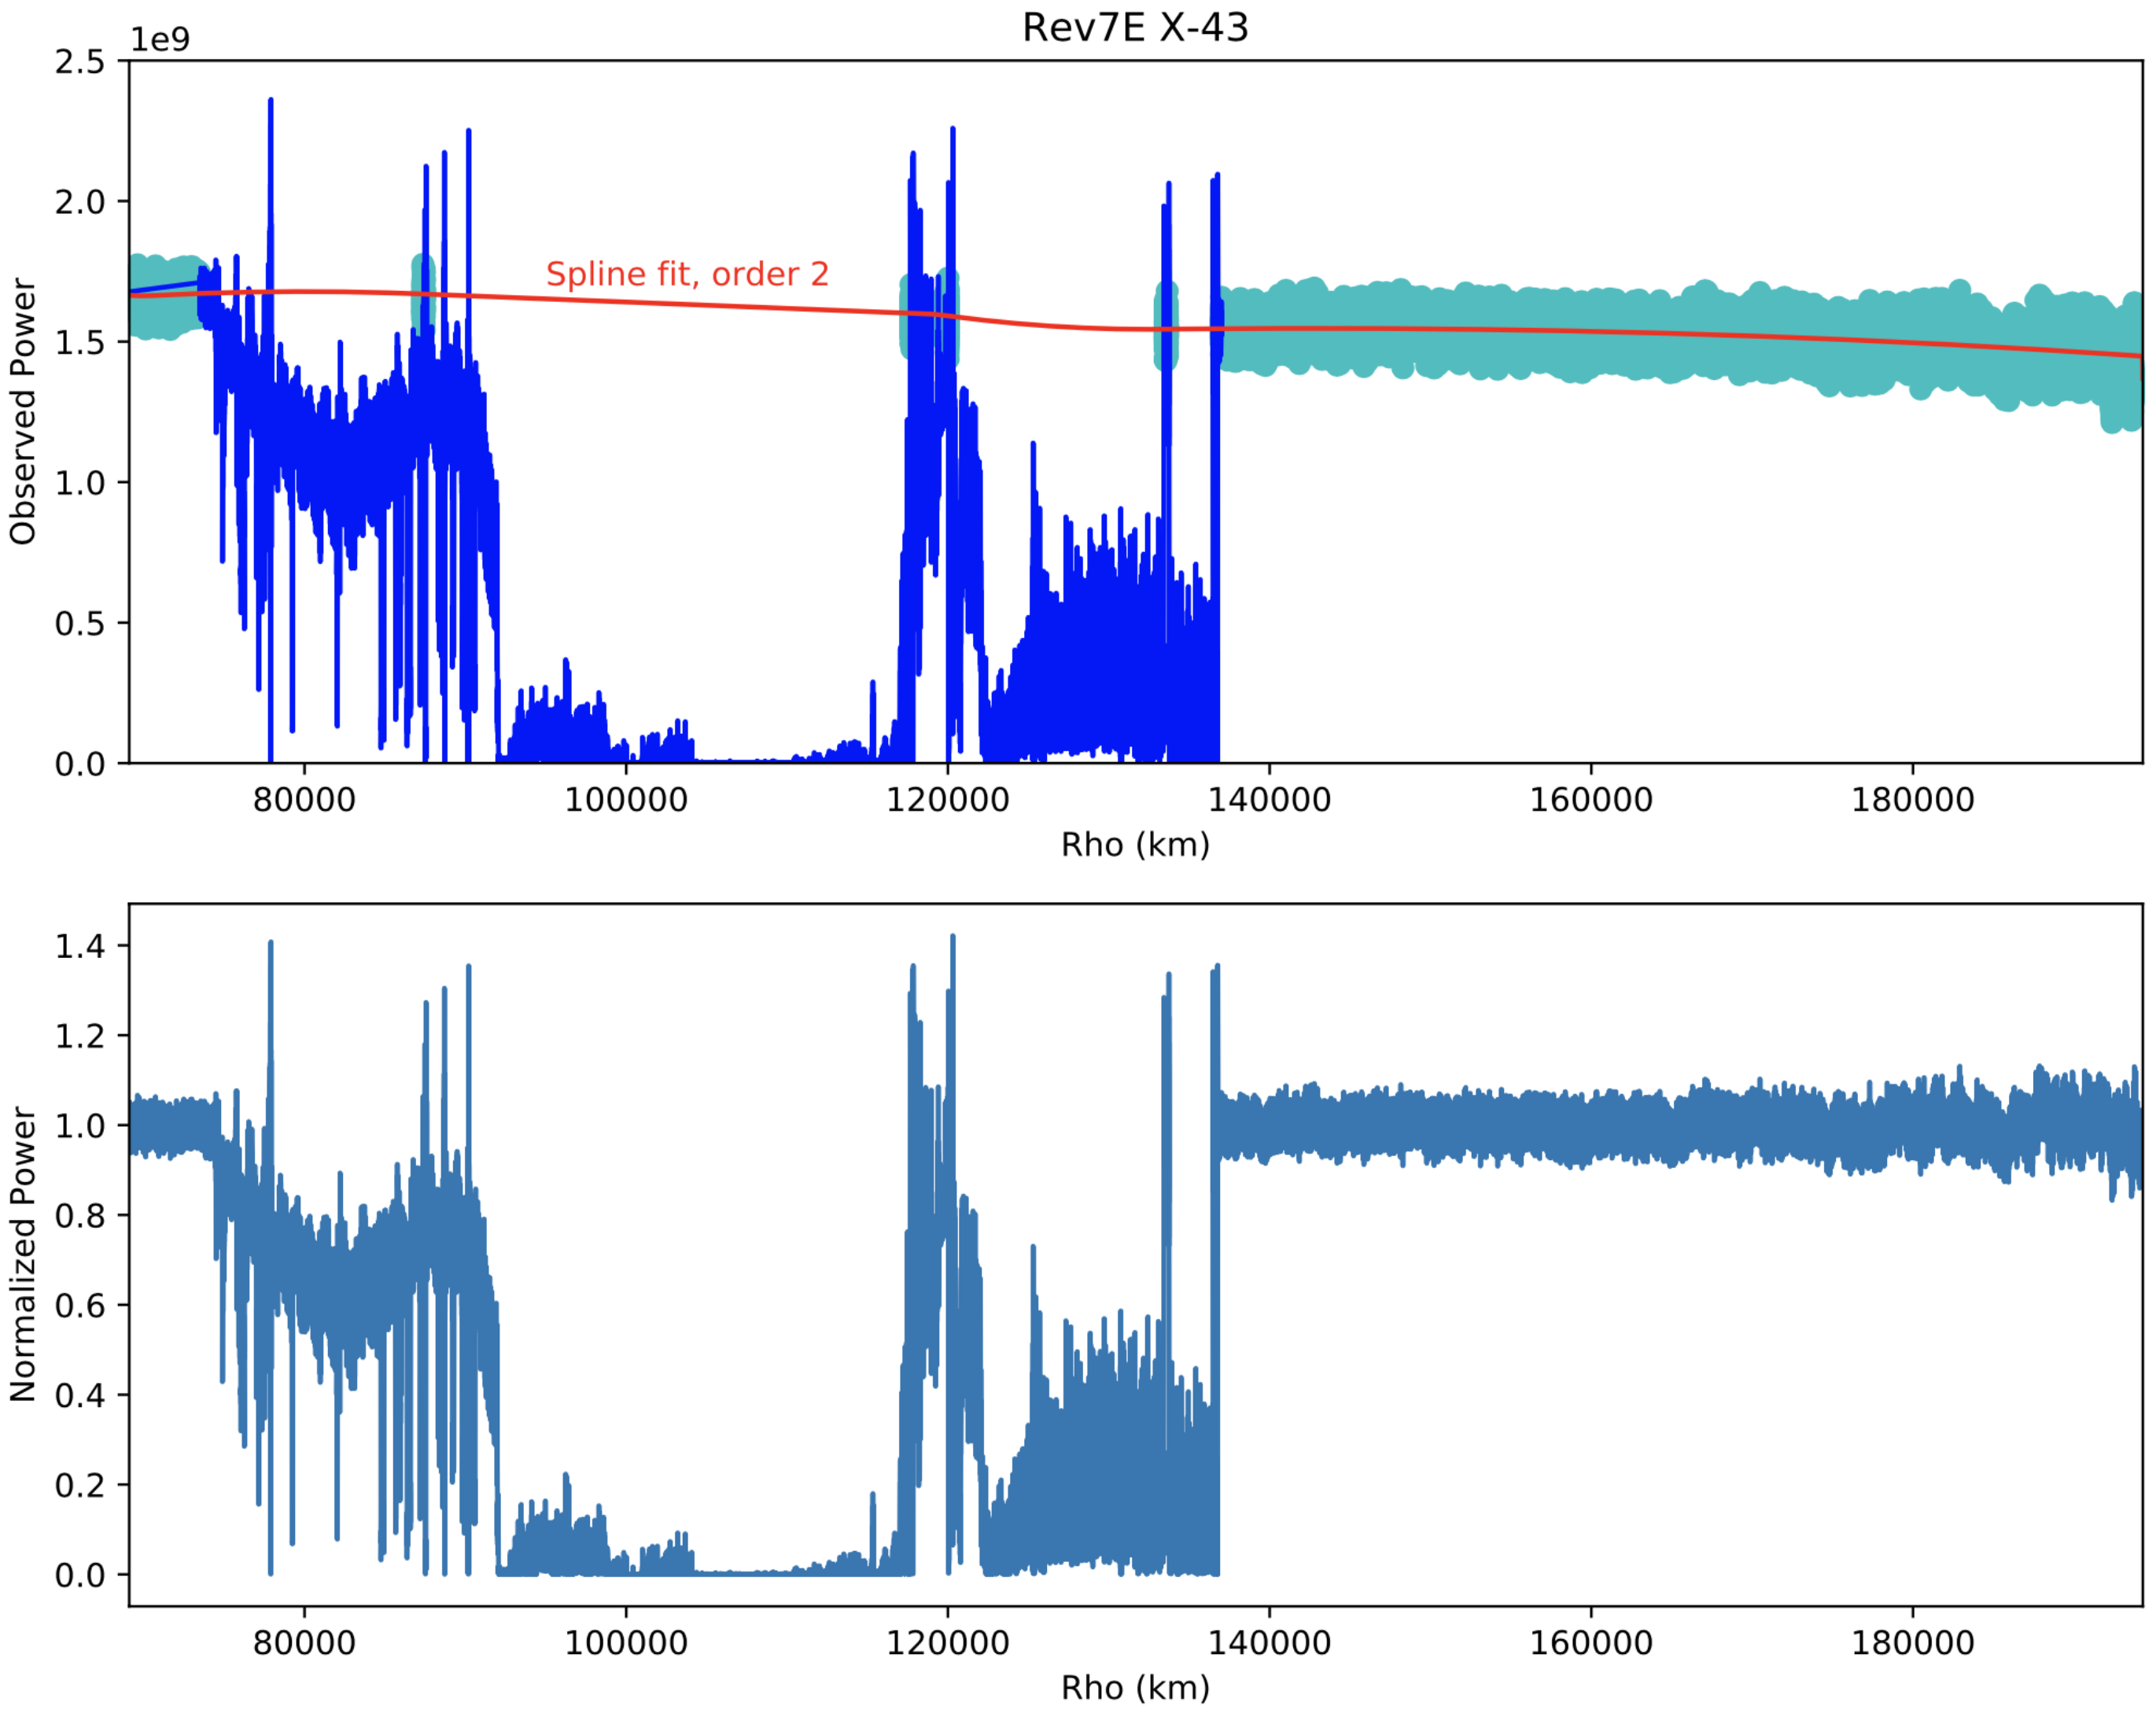
\includegraphics[trim = {0.0in 0.5in 0.0in 0.75in},clip, width=0.88\textwidth]{gjs_rev7E_X43_make_P_norm_vals}
    \caption[Power normalization in Python]{Illustration of the calculation and application of power normalization, using a 2nd-order \gls{least squares} \gls{spline fit} in Python. The upper panel shows the power prior to normalization, with the red curve showing the spline fit to the free-space regions shown in cyan. The lower panel shows the observed power after normalization by the spline fit.}
    \label{fig:python_spline}
\end{figure}
In the top panel of Fig.~\ref{fig:python_spline}, we show observed power, resampled to uniform radius at 250 m spacing, in blue. The selected free-space regions used to constrain the fit are highlighted in light blue, and the second-order spline fit to the data uniformly spaced time is shown in red. The bottom panel of Fig.~\ref{fig:python_spline} shows the power after normalizing the blue curve in the top panel with the spline fit. Notice that, after this process, the free space regions throughout the entire range included in the fit have been normalized to unity. The normalized complex transmittance produced in this process is the diffraction pattern (both power and phase) that we will use as input to the Fresnel inversion procedure that corrects for diffraction and retrieves the radial optical depth profile responsible for the observed diffraction pattern.\par
We now compare the Python-produced diffraction pattern discussed just above with that of Marouf for the same data set. Additionally, in order to see how well this new method of normalizing and resampling transfers to the inverted result, we apply diffraction reconstruction using the inversion software we developed in IDL. By means of illustration, we show the results for the Maxwell Ringlet, which has high internal optical depth and wavelike radial structure that we would like to capture in the diffraction reconstruction. Figure~\ref{fig:inversion_of_python_tau} shows the pre- and post-correction optical depth, and Fig.~\ref{fig:inversion_of_python_phase} shows the corresponding results for phase. Each of these two figures shows Marouf's results in magenta, our calculations in black, and the difference between them in green. Overall, the agreement between the two independent analyses is excellent, with the retrieved optical depth profiles overlying each other almost perfectly. The differences in the phase are due primarily to the small difference in residual frequency correction between the two analyses, resulting a differential drift, or slope, in the phase residual, as can clearly be seen in the green line in both panels of Fig.~\ref{fig:inversion_of_python_phase}.
\begin{figure}[H]
    \centering
    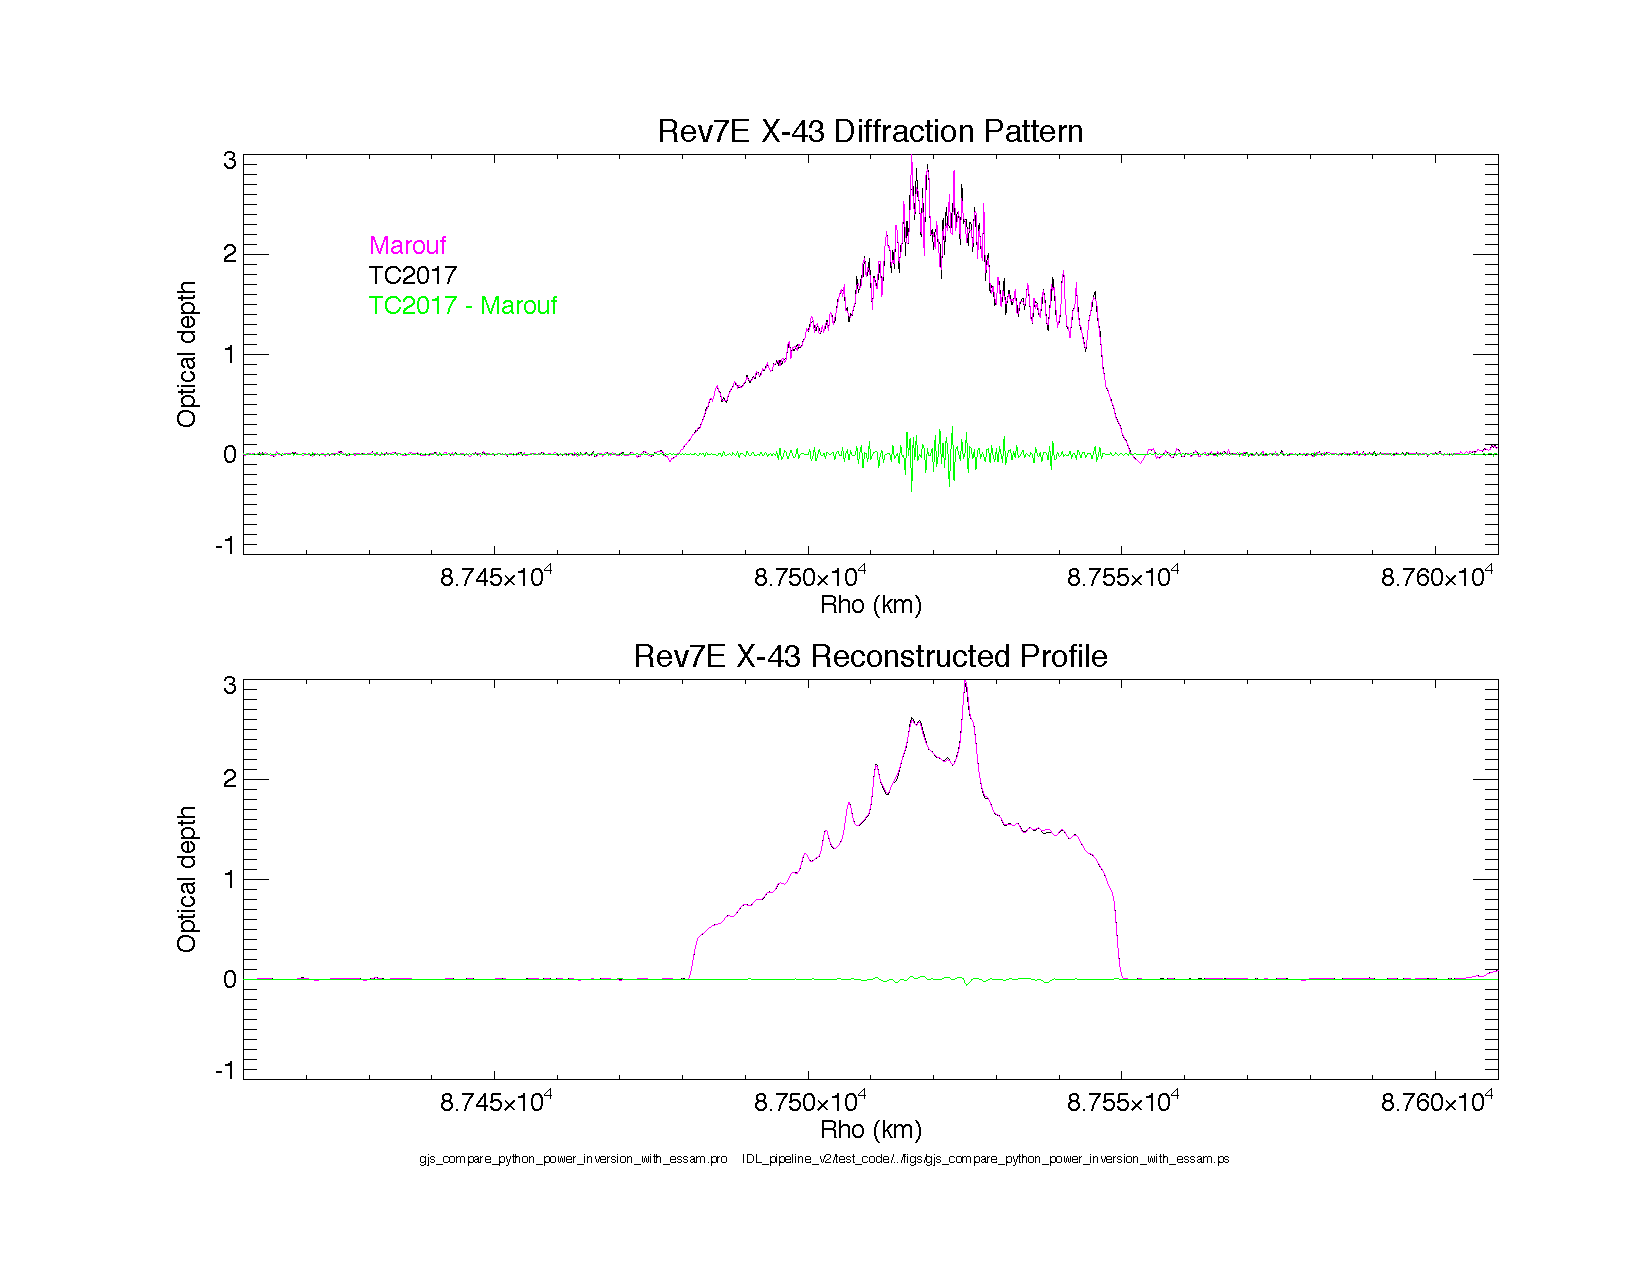
\includegraphics[page=1,trim = {0.0in 0.82in 0.0in 0.75in},clip, width=0.9\textwidth]{gjs_compare_python_power_inversion_with_essam.pdf}
    \caption[Maxwell Ringlet profiles using Python normalization and resampling]{Optical depth as produced from normalization and resampling in Python (top black curve) and its diffraction corrected profile (bottom black curve), zoomed in on the Maxwell Ringlet. For comparison, we plot Marouf's raw and inverted optical depth in magenta, as well as the difference between the two profiles in green.}
    \label{fig:inversion_of_python_tau}
\end{figure}
\begin{figure}[H]
    \centering
    \includegraphics[page=2,trim = {0.0in 0.82in 0.0in 0.75in},clip,width=0.9\textwidth]{gjs_compare_python_power_inversion_with_essam.pdf}
    \caption[Maxwell Ringlet phase using Python normalization and resampling]{Phase used for the inversion in Fig.~\ref{fig:inversion_of_python_tau} (top), and its diffraction corrected profile (bottom), using the same color scheme as before.}
    \label{fig:inversion_of_python_phase}
\end{figure}
\begin{figure}[H]
    \centering
    \includegraphics[page=3,trim = {0.0in 0.82in 0.0in 0.75in},clip, width=0.9\textwidth]{gjs_compare_python_power_inversion_with_essam.pdf}
    \caption[Comparison of Marouf's inversion and our independent analysis]{The top panel is the inversion of our optical depth (black) and our inversion of Marouf's raw optical depth (cyan), as well as the difference between the two (green). Inverted phase for each profile, as well as the difference between them, is shown in the bottom panel using the same color scheme.}
    \label{fig:inversion_of_python_vs_essam}
\end{figure}
Finally, we performed Fresnel inversion using Marouf's diffraction pattern optical depth and phase and compared it to the inversion of our diffraction pattern optical depth and phase. This is to test the quality of the Python resampling and normalization steps independently of the quality of our Fresnel inversion relative to Marouf's. Figure~\ref{fig:inversion_of_python_vs_essam} shows the results, with black as the reconstruction of our data, cyan as the reconstruction of Marouf's data, and green as the difference between the two. For reference, note that the black optical depth curve is the same as that in the bottom panel of Fig.~\ref{fig:inversion_of_python_tau} and the black phase curve is the same as that in the bottom panel of Fig.~\ref{fig:inversion_of_python_phase}. Once again, the agreement is quite satisfactory.\par
On the basis of these tests, we conclude that our frequency correction and normalization procedures in Python give excellent agreement with Marouf's, and our IDL Fresnel inversion routines also give results comparable to Marouf's. The next steps in our translation will be to convert the geometry calculations from IDL to Python, which should be straightforward, using the NAIF toolkit in Python, and the Fresnel inversion routine from IDL to Python, which will require careful comparison of IDL and Python array arithmetic and FFT's, but otherwise should similarly be straightforwrd. In short, we are well on our way to having a Python-only data processing pipeline that gives results comparable to those in hand produced by Marouf's software.
\subsection{Documentation}
We will submit our open-source software and documentation to the existing GitHub repository {\tt https://github.com/NASA-Planetary-Science/rss\_ringoccs}. An installation manual and a ``Getting Started" user's guide will provide clear instructions and examples for both End-to-End and Quick-Look processing of representative data sets, for users who want to get started quickly, without worrying about the detailed mathematics behind the data pipeline.\par
For users who want to understand the processing steps from beginning to end, we will also provide a more detailed guide to the physics and mathematics of diffraction reconstruction. Based on our experience in developing this software, we often found that an explanation of a certain principle, or an intermediate equation, was lacking, making the development of an algorithm difficult. In particular, an understanding of the mathematics of Fourier analysis and convolution theory is required, as well as an in-depth appreciation of Fourier optics and the Fresnel-Fraunhofer principle, but this material not easily accessible, being instead spread across dozens of papers and other references. This detailed guide is based on our experience of learning the material, and we hope it will be useful for scientists who wish to have an understanding of the diffraction theory behind the code we have developed, including its limitations, so that future improvements can be made.\par
We outline below our planned comprehensive documentation:
\setlength{\columnsep}{1cm}
\begin{itemize}[leftmargin=0pt]
\begin{multicols}{2}
    \item[] Contents
    \item[1] Geometry
    \begin{itemize}
        \item[1.1] Basic Theorems and Definitions
        \item[1.2] The Geometry of an Occultation
        \begin{itemize}
            \item[1.2.1] Ingress Occultations
            \item[1.2.2] Egress Occultations
            \item[1.2.3] Chord Occultations
        \end{itemize}
        \item[1.3] How to Use the NAIF Toolkit
    \end{itemize}
    \item[2] Data Processing
    \begin{itemize}
        \item[2.1] Basic Theorems and Definitions
        \item[2.1] The Mathematics of Spline Fitting and Curve Fits
        \item[2.2] Retrieval of the Sky Frequency
        \item[2.3] Retrieval of the Complex Transmittance
        \item[2.4] Normalization of the Power
    \end{itemize}
    \item[3] Fresnel Inversion
    \begin{itemize}
        \item[3.1] Basic Theorems and Definitions
        \begin{itemize}
            \item[3.1.1] A Primer on Fourier Analysis
            \item[3.1.2] A Primer on Complex Analysis
            \item[3.1.3] A Primer on Convolution Theory
            \item[3.1.4] A Primer on Approximation Theory and Stationary Phase
        \end{itemize}
        \item[3.2] The Fresnel-Fraunhofer Theory 
        \begin{itemize}
            \item[3.2.1] The Maxwell Theory
            \item[3.2.2] The Fresnel Diffraction Equation
            \item[3.2.3] The Fresnel Approximation
        \end{itemize}
        \item[3.3] Fresnel Inversion
        \begin{itemize}
            \item[3.3.1] Use of FFTs and the Convolution Theorem
            \item[3.3.2] Use of Direct Integration
            \item[3.3.3] Use of Fredholm Inversion Techniques
        \end{itemize}
        \item[3.4] Problems with Fresnel Inversion
            \begin{itemize}
                \item[3.4.1] Poor Phase Retrieval
                \item[3.4.2] Poor Power Retrieval
                \item[3.4.3] Violating the Sampling Theorem
                \item[3.2.4] Window Types
                \begin{itemize}
                    \item [3.2.4.1] Problems with Window Sizes
                \end{itemize}
            \end{itemize}
    \end{itemize}
    % \item[4] IDL Codes
    % \begin{itemize}
    %     \item[4.1] The Codes
    %     \item[4.2] Examples
    % \end{itemize}
    \item[4] Python Codes
    \begin{itemize}
        \item[5.1] The Codes
        \item[5.2] Examples
    \end{itemize}
    \item[5] Catalog
    \item[] Glossary
    \item[] Index
\end{multicols}
\end{itemize}
\section{Future Milestones and Delivery Schedule}
\label{section:future milestones and delivery shedule}
We outline below the major milestones we envision for this archive project, including target dates for completion. 
\begin{itemize}
    \item{2018 Feb 14} -- This Interim Report to JPL/Cassini and \gls{pds} Ring-Moon Systems Node.
    \item{2018 Feb 14} -- Reproduce {\tt CORSS\_8001/EASYDATA/Rev07E\_RSS\_2005\_123\_X43\_E} and associated summary, geometry, and calibration files.
    \item{2018 Feb 14} -- Submit proposed organization of {\tt CORSS\_8101} archive volume to the \gls{pds} Ring-Moon Systems Node.
    \item{2018 April 30} -- Submit sample archive volume {\tt CORSS\_8101} to \gls{pds} for peer review, with complete set of contents for Rev007E at 0.5 and 1.0 km resolution at S, X, and Ka band.
    \item{2018 April 30} -- Submit GitHub {\tt rss\_ringoccs} Python software package for peer review by \gls{pds}.
    \item{2018 June 30} -- Revised sample archive volume {\tt CORSS\_8101}, incorporating any revisions in response to peer review, and adding selected multi-wavelength examples of RSS occultation observations of inner C ring and F ring at high spatial resolution.
    \item{2018 June 30} -- Submit revised/final Python software package to GitHub, based on recommendations from peer review.
    \item{2018 June 30 to Aug 31} -- Pipeline processing and submission to \gls{pds} of 0.5 and 1.0 km diffraction-corrected data at S, X, and Ka band.
    \item{2018 Aug 31} -- Final date for submissions to \gls{pds}.
\end{itemize}
\end{document}